\documentclass{article}
\usepackage{graphicx, amsmath, amssymb, hyperref, enumitem, subcaption}
\usepackage{algorithm,algorithmicx,algpseudocode}

\usepackage{tikz}
\usetikzlibrary{arrows,automata,positioning}

\usepackage[bottom]{footmisc}
\usepackage[margin=1in]{geometry}
\title{Impianti di elaborazione}

\author{Giuseppe Capasso}

\begin{document}

\maketitle

\tableofcontents
\newpage

\section{Performance di un sistema}
Valutare le prestazioni di un sistema di calcolo è un problema principale per confrontare
diversi sistemi che svolgono funzionalità simili. Infatti, l'obiettivo principale di utenti
, amministratori e aziende è ottenere il proprio obiettivo o le migliori performance con
costi minimi. Per eseguire una corretta valutazione delle performance diun sistema bisogna
avere in mente un obiettivo in base al quale bisogna costruire l'esperimento. 
\begin{itemize}
  \item Scelta delle metriche, tecniche di valtuazione e workload di un sistema;
  \item Esecuzione corretta delle misure;
  \item Uso delle tecniche statistiche giuste per valutare i risultati degli esperimenti;
\end{itemize}

Un sistema può essere valutato in tre modi:
\begin{enumerate}
  \item \textbf{Simulazione}: una tecnica simulativa prevende l'utilizzo di un simulatore
    che esegue le operazioni del sistema prendendo input randomici. La simulazione può 
    essere vantaggiosa perchè non richiede il sistema in funzione, ma può essere complicata 
    da realizzare. Può essere flessibilee automatizzabile, ma può risultare molto costosa;
  \item \textbf{Analitcamente}: una tecnica analitica prevede l'adozione di un modello 
    teorico che non richiede la presenza del sistema o di un suo prototipo funzionante. 
    Tipicamente, viene utilizzata la teoria delle code che risulta abbastanza semplice da 
    produrre risultati in forma chiusa;
  \item \textbf{Misure dirette}: basarsi su misure dirette può portare a risultati 
    realistici, ma queste tecniche hanno bisogno di un prototipo funzionante. Inoltre,
    l'utilizzo di tecniche errate può portare a risultati fuorvianti. Il processo 
    di misurazione, infatti, è fonte di imprecisioni e comporta un costo dato, 
    per esempio, anche dagli strumenti di misura necessari.
\end{enumerate}

Nella realtà, è utilizzata una combinazione delle tecniche per controllare i risultati
e analizzare il sistema durante tutta la fase di progettazione.

\subsection{Metriche}
Le metriche rappresentano i fattori utilizzati per trarre le conclusioni sulla valutazione 
delle performance del sistema. In particolare, in base allo scopo dell'esperimento, saranno 
selezionate metriche significative. Ad esempio, se un sistema presenta degli errori non ha
senso misurare il tempo di risposta in quanto questo sarà condizionato dagli errori presenti. 
In Figura \ref{fig:metric_overview}, è mostrata una panormaica delle metriche in cui si 
distingue due tipologie:
\begin{itemize}
  \item Sistema corretto: le metriche utilizzate sono \textit{response time},
    \textit{throughput}, \textit{resource utilization}. In questa fase, è possibile
    identificare il \textbf{bottlneck} del ssitema, identificato come la risorse 
    più utilizzata nel sistema;
  \item Sistema con errori: in questo caso è utile calcolare metriche quali
    \textit{reliability}, \textit{availbability}. Inoltre, è utile modellare la 
    distruzione degli errori;
\end{itemize}

\begin{figure}
  \begin{center}
    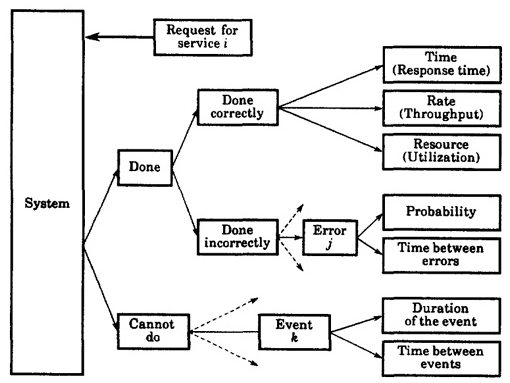
\includegraphics[width=.5\textwidth]{./figures/metrics_overview.png}
  \end{center}
  \caption{Panoramica delle metriche da utilizzare in base al sistema}
  \label{fig:metric_overview}
\end{figure}

In generale, le metriche sono di tre tipi (riassunti in \ref{fig:metric_types}):
\begin{itemize}
  \item \textbf{HB}: higher is better;
  \item \textbf{LB}: lower is better;
  \item \textbf{NB}: nominal is best; 
\end{itemize}

\begin{figure}
  \begin{center}
    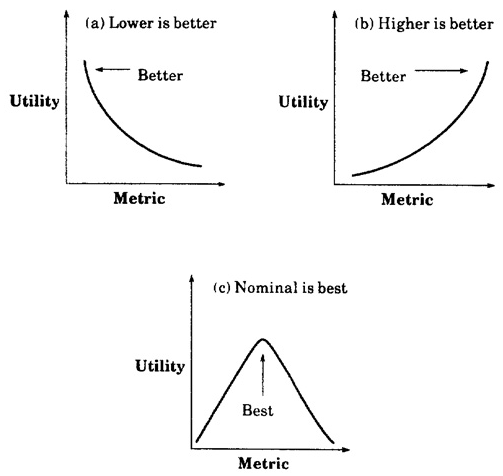
\includegraphics[width=.6\textwidth]{./figures/metrics_type.png}
  \end{center}
  \caption{Tipi di metriche}\label{fig:metric_types}
\end{figure}


\paragraph{Response time} Il tempo di risposta di un sistema è definitp come l'intervallo 
di tempo tra la richiesta di un utente e la risposta del sistema. Questa metrica può essere
soggetta ad ambiguità in quanto l'invio della richiesta e la ricezione della risposta può 
non essere istantaneo. Quindi bisogna sempre specificare cosa si intende per tempo di 
risposta. Per un sistema \textit{batch} si parla di tempo di \textit{turnaround}; per altri
sistemi, l'intevallo di tempo che intercorre tra l'invio di una richiesta e l'inizio della
risposta è detto tempo di reazione (Figura \ref{fig:response_time_definition}).

\begin{figure}
  \begin{center}
    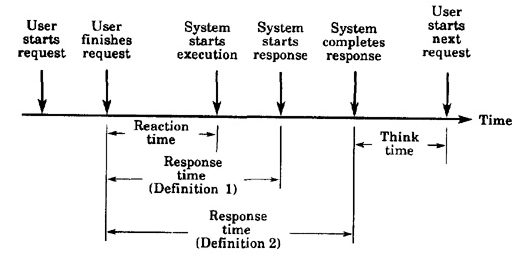
\includegraphics[width=.6\textwidth]{./figures/response_time_definition.png}
  \end{center}
  \caption{Definizioni del tempo di risposta}\label{fig:response_time_definition}
\end{figure}

Il tempo di risposta di un sistema aumenta con l'aumentare del carico. Il rapporto tra il 
response time con un certo carico $R_L$ e quello con il carico minimo $R_{min}$ è detto 
\textit{stretch factor}. $$stretch = \frac{R_L}{R_{min}}$$

\paragraph{Throughput}
Il throughput indica quante richieste per unità di tempo possono essere servite in un unità
di tempo. La sua unità di misura può variare a seconda del sistema sotto test: 
\textit{millions of instruction per second} o \textit{millions of floating point operations
per second} (usati per le CPU); \textit{packets per second} o \textit{bits per second}
(utilizzate per la reti). Il throughput cresce all'aumentare del carico fino ad arrivare ad
un punto detto \textbf{\textit{usable capacity}} per poi fermarsi o cominiciare a diminuire.
Il limite teorico per un sistema con workload reale è detto \textit{Nominal Capacity}. 
Il gomito della curva del througput è detto \textit{knee capacity}. Il rapporto usable 
capacity e nominal capacity è detto efficienza. $$eff = \frac{usable\; capacity}{nominal\; 
capacity}$$. Un esempio di andamento del troughput è in Figura 
\ref{fig:throughput_definition}; mentre un esempio di efficienza è riportata in 
\ref{fig:efficiency_example}.

\begin{figure}
  \begin{center}
    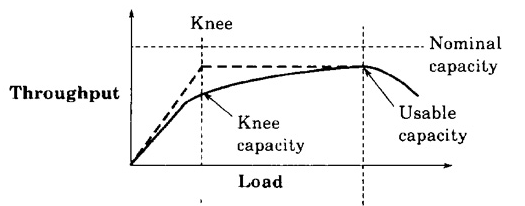
\includegraphics[width=.6\textwidth]{./figures/throughput_definition.png}
  \end{center}
  \caption{Definizione del throughput}\label{fig:throughput_definition}
\end{figure}

\begin{figure}
  \begin{center}
    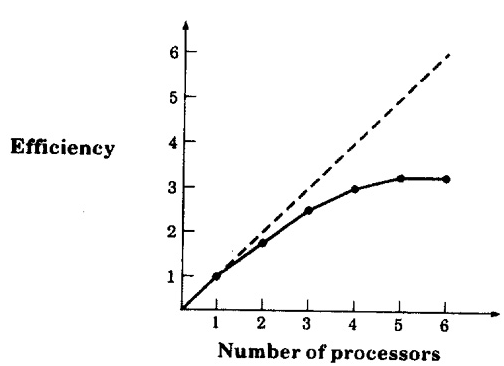
\includegraphics[width=.6\textwidth]{./figures/efficiency_definition.png}
  \end{center}
  \caption{Esempio di efficienza}\label{fig:efficiency_example}
\end{figure}

In alcuni esperimenti, viene definita la \textbf{potenza} di un sistema come il rapporto 
tra throughput e response time. Infatti, si vede che il punto di \textit{knee capacity} 
corrisponde al massimo della potenza. $$power = \frac{throughput}{response\; time}$$

\paragraph{Utilizzazione}
L'utilizzazione di una risorsa è misurata come la porzione di tempo in questa risulta 
occupata per servire una richiesta. Al contrario, l'intervallo di tempo in cui non viene
usata è detto \textbf{\textit{idle time}}.

\paragraph{Fairness Index}
Nei sistemi multiutente, può essere necessario che tutti gli utenti sono trattati in 
maniera equa o, meglio ancora, che nessun utente monopolizzi il sistema. Questa metrica 
misura il throughput teorico assegnato a ciascun utente con quello effettivamente misurato. 
L'indice di \textit{fairness} è definito secondo la Equazione \ref{eq:fairness_index}.

\begin{equation}
  f(x_1,x_2,\dots, x_n) = \displaystyle\frac{(\sum_{i=1}^{n}x_i)^2}{n \sum_{i=1}^{n}x_i^2}
  \label{eq:fairness_index}
\end{equation}

Si tratta di una quantità compresa tra $0$ e $1$. Con $x_i$, si indica il throughput 
effettivo (misurato) nornmalizzato rispetto a quello teorico (quello \textit{fair}), come 
illustrato in Equazione \ref{eq:norm_throughput}.

\begin{equation}
  x_i = \frac{T_i}{F_i} \; \forall i = 1,2\dots n
  \label{eq:norm_throughput}
\end{equation}

\subsection{Workload}
Un \textit{workload} è un insieme di test che ha lo scopo di generare dati utili a calcolare
le metriche presentate nella sezione precedente su un sistema. I workload si distinguono in:
\begin{itemize}
  \item reale: consiste delle reali richieste che vengono ricevute dal servizio e sono 
    inviate da utenti reali. Questo workload può avere dati sensibili, può essere difficile
    da trattare e da ottenere;
  \item sintetico: è generato in maniera artificiale a partire dalle specifiche del sistema.
    Può essere configurato, ma non contiene dati sensibilie. Il problema dell'utilizzare un 
    workload sintetico sta nel fatto che questo potrebbe non essere rappresentativo del 
    sistema reale;
\end{itemize}


\subsubsection{Tipi di Workload}
Esistono diversi tipi di workload. I più vecchi mirano a testare le performance di
processori, quindi si basano su istruzioni o mix di istruzioni. Per sistemi più complessi,
si usano applicazioni che sfruttano più componenti del sistemi.

\paragraph{Addition Instruction} Per i primi processori che avevono poche istruzioni,
quella di addizione era la più usata. Questo workload usa solo le istruzioni di addizione 
e usa come metrica di performance;

\paragraph{Instruction mix} Questo tipo workload consente di usare diverse tipi di 
istruzioni specificando intervalli di tempo, numero di occorrenze nel workload. Questo 
approccio porta svantaggi, ma i sistemi moderni sono complicati ed è difficile coprire 
tutte le istruzioni. Il tempo di risposta delle istruzioni dipende dallo stato della 
pipeline, dai tempi di accesso alla memoria, dalla cache e dalle modalità di indirizzamento.

\paragraph{Kernel} Un kernel è un insieme di istruzioni che costituisce una funzione di alto
livello. In particolare, i ricercatori includono le funzioni più utilizzate nei kernel.
Questa tecnica risolve il problema del \textit{instruction mix}, in quanto non si vede più
la singola istruzione come isolata, ma in generale si usa una funzione "vicina" al workload
reale del sistema per misurarne le perfomance. Di solito, i kernel sono funzioni che non 
includono operazioni di I/O e per questo sono detti \textit{processing kernel} e sono una 
forma più generalizzata di \textit{instruction mix}. 

\subsubsection{Benchmark}
Un \textbf{benchmark} è un particolare workload che è stato standardizzato per essere usato
come strumento per estrarre metriche per confrontare sistemi differenti. L'applicazione di
un benchmark per comparare due o più sistemi è detta \textbf{\textit{benchmarking}}.

Un benchmark deve essere:
\begin{itemize}
  \item rappresentativo;
  \item portabile;
  \item scalabile;
  \item ripetibile;
  \item facile da capire;
  \item facile da usare;
\end{itemize}

\subsubsection{Benchmark più famosi}
I benchmark più famosi testano parti fondamentali di un sistema quali gestore dello stack,
FPU\dots.

\paragraph{Ackermann's Function}
Questo benchmark misura l'efficienza del sistema di chiamata delle procedure e dello stack.
In Figura \ref{fig:ackermann}, si vede come la funzione di ackermann in realtà sia definita 
in maniera ricorsiva. Essa può essere configurata attraverso due numeri positivi $m$, $n$.

\begin{figure}
  \begin{center}
    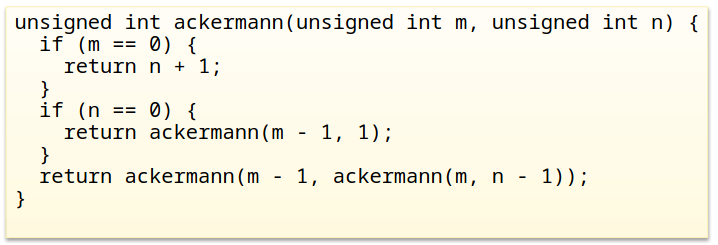
\includegraphics[width=.5\textwidth]{./figures/ackermann_example.png}
  \end{center}
  \caption{Esempio della funzione di Ackermann}\label{fig:ackermann}
\end{figure}

Questo benchmark estrai il tempo medio di esecuzione per chiamata, il numero di istruzioni 
eseguite per chiamata e spazio occupato nello stack per chiamata. 

\subsection{Esempio: performance di un sistema cloud}
Con \textbf{\textit{cloud computing}}, si intende un modello che fornisce agli utenti un 
accesso on demand a un pool di risorse condivise configurabili (rete, server, storage) 
che può essere gestito con uno sforzo minimo senza interazione dal fornitore.

Secondo il NIST, un'infrastruttura cloud è una collezione di elementi hardware e software 
con le seguenti $5$ caratteristiche:
\begin{enumerate}
  \item \textbf{\textit{On-demand self service}}: un utente può richiedere servizi senza 
    interazione del \textbf{\textit{service-provider}};
  \item \textbf{\textit{Broad network access}}: i servizi offerti possono essere acceduti 
    attraverso la rete e deve essere favorita l'eterogeneità dei client;
  \item \textbf{\textit{Resource pooling}}: le risorse del \textit{provider} sono condivise
    per servire più utenti con un modello \textbf{\textit{multi-tenant}}. Un utente accede 
    può essere assegnato a differenti risorse fisiche o virtuali in base alla sua richiesta;
  \item \textbf{\textit{Rapid elasticity}}: dal punto di vista del cliente la capacità di un 
    archittura cloud deve sembrare infinita. Un'infrastruttura cloud deve essere capace di 
    aumentare o rilasciare risrorse in base alla richiesta;
  \item \textbf{\textit{Measured service}}: un'infrastruttura cloud deve essere in grado di 
    controllare e ottimizzare automaticamente le risorse attraverso un sistema di monitoraggio 
    in maniera trasparente alle richieste dell'utente;
\end{enumerate}

\subsubsection{Tipi di cloud}
Nella storia si sono formati diversi modelli per caratterizzare i sistemi cloud. I più usati 
sono quelli detti \textbf{\textit{deployment models}} e \textbf{\textit{service models}}:

\paragraph{Deployment models} Questi modelli effettuano una distinzione in base a come si 
accede al cloud. In generale, si definiscono le seguenti categorie:
\begin{itemize}
  \item \textbf{\textit{Private cloud}}: infrastruttura a uso esclusivo di una singola 
    organizzazione e può essere acceduta solo da un gruppo di utenti ristretto. Può essere 
    gestita dall'organizzazione stessa, da una di terze parti e può esistere sia 
    \textbf{\textit{on-premise}}\footnote{Con il termine on-premise, si intende l'installazione 
    di un'infrastruttura dedicata allo scopo dell'orgnaizzazione.} che non;
  \item \textbf{\textit{Community cloud}}: infrastruttura gestita da un gruppo di utenti
    che hanno interessi in comune;
  \item \textbf{\textit{Public cloud}}: un'infrastruttura gestita e posseduta da un ente
    pubblico, un'organizzazione privata \dots. Tutti gli utenti possono accedere ai servizi.
    L'infrastruttura esiste on-premise del provider;
  \item \textbf{\textit{Hybrid cloud}}: l'infrastruttura è la composizione di una o più 
    delle architetture dette prima che rimangono entità separate, ma che sono unite da 
    tecnologie proprietarie che abilitano la comunicazione e la portabilità di dati e 
    applicazioni;
\end{itemize}

\paragraph{Service models} Questi modelli fanno riferimento al tipo di servizio offerto 
attraverso il cloud:
\begin{itemize}
  \item \textbf{\textit{IaaS} (Infrastracture as a service)}: in questo tipo modello 
    il cloud provider fornisce all'utente servizi base come: 
    \begin{itemize}
      \item Server e storage;
      \item Networking e security;
      \itemm Data center ed edifici fisici;
    \end{itemize}
  \item \textbf{\textit{PaaS} (Platform as a service)}: in questo tipo modello 
    il cloud provider fornisce all'utente servizi da utilizzare per creare le proprie 
    applicazioni:
    \begin{itemize}
      \item Sistemi operativi;
      \item Database;
      \itemm Analitycs;
    \end{itemize}
  \item \textbf{\textit{SaaS} (Software as a service)}: in questo tipo modello 
    il cloud provider fornisce all'utente direttamente applicazioni funzionanti da utilizzare 
    attraverso la rete.
\end{itemize}

\subsubsection{Capacity planning}
Non è una buona idea allocare staticamente le risorse di un sistema cloud in quanto la loro 
richiesta può avere un'alta variabilità nel tempo. Ad esempio, in Figura 
\ref{fig:cloud-res-utilization}, è mostrato l'utilizzo di una risorsa durante l'arco della 
giornata. Si nota che che durante le notte le risorse utilizzate sono molto meno rispetto 
alla giornata. Un'allocazione statica significa:
\begin{itemize}
  \item Sprecare le risorse durante le ore notturne, se allocate durante il picco giornaliero;
  \item Non riuscire a soddisfare la domande durante il giorno, se allocate secondo la 
    richiesta notturna;
\end{itemize}

Chiaramente, la soluzione a questo problema è un'allocazione dinamica delle risorse.
\begin{figure}
  \begin{center}
    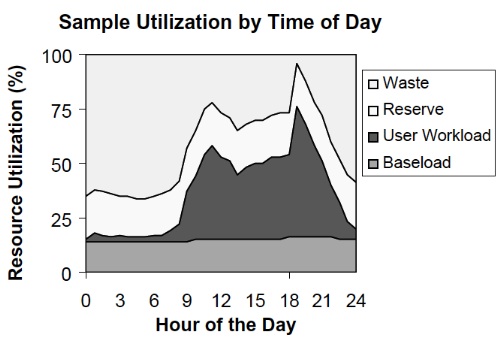
\includegraphics[width=.75\textwidth]{figures/cloud-resource.png}
  \end{center}
  \caption{Risorsa utilizzata durante una giornate in un'infrastruttura cloud}
  \label{fig:cloud-res-utilization}
\end{figure}

È molto difficile effettuare il capacity planning di un'infrastruttura cloud in quanto
bisogna trovare il giusto compromesso tra \textbf{\textit{QoS} (quality of service)} e spesso 
confrontarsi con eventi imprevedibili come lo \textbf{\textit{Slashdot effect}}.

\paragraph{Rapid elasticity} La principale proprità del cloud è quella di allocare risorse 
addizionali laddove alcune applicazioni le richiedano e di riprenderne possesso quando non 
sono più richieste. Questa proprità è detta \textbf{\textit{rapid elasticity}} e può essere
utilizzata per fa crescere la capacità di un'infrastruttura cloud. In particolare, esistono 
$3$ modi per aumentare la capacità (Figura \ref{fig:cloud-rapid-elasticity}):
\begin{enumerate}
  \item Crescita verticale: ad ogni VM è possibile allocare più risorse quali CPU, memoria 
    e risorse di rete;
  \item Crescita orizzontale: si creano più VM per gestire il carico di richieste;
  \item \textbf{\textit{Outhgrowth}}: altre risorse indipendenti si aggiungono all'
    infrastruttura anche provenienti da altri datacenter geograficamente distanti;
\end{enumerate}

\begin{figure}
  \begin{center}
    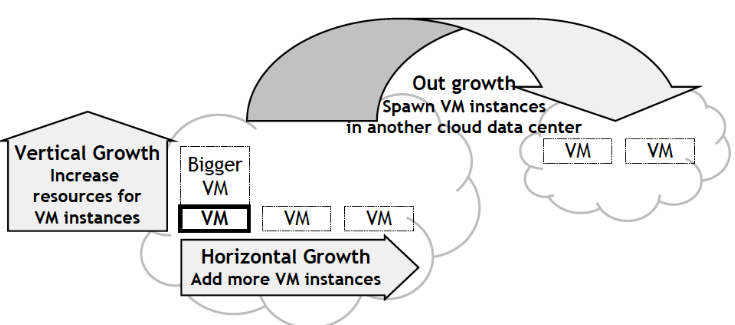
\includegraphics[width=.6\textwidth]{figures/cloud-rapid-elasticity.png}
  \end{center}
  \caption{Esempi di strategie per aumentare la capacità di un'infrastruttura cloud}
  \label{fig:cloud-rapid-elasticity}
\end{figure}

\paragraph{Slashdot effect} Lo slashdot effect si verifica quando un sito con molti utenti
crea un collegamento a uno molto piccolo realizzando un grande incremento del traffico di 
quest'ultimo (Figura \ref{fig:cloud-slashdot}). Chiaramente, questo effetto è imprevedibile 
sia per il carico ricevuto dal sito che per l'istante in cui occorre.

\begin{figure}
  \begin{center}
    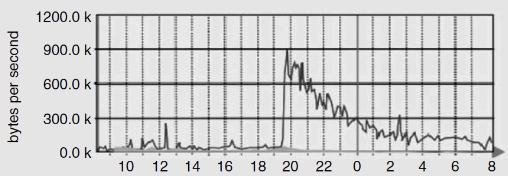
\includegraphics[width=.75\textwidth]{figures/cloud-slashdot-effect.png}
  \end{center}
  \caption{Traffico ricevuto da un sito soggetto a slashdot effect}
  \label{fig:cloud-slashdot}
\end{figure}

\paragraph{Nominal cloud capacity model}
Nel modello mostrata in Figura \ref{fig:cloud-spare-capacity}, si divide la capacità 
dell'infrastruttura in $2$ tipi:
\begin{itemize}
  \item \textbf{Engaged online capacity}: quella che può essere offerta agli utenti con 
    una qualità del servizio accettabile e affidabile;
  \item \textbf{Spare online capacity}: la capacità che può essere immediatamente richiesta 
    dalle applicazioni ma che al momento non viene utilizzata attivamente;
\end{itemize}

\begin{figure}
  \begin{center}
    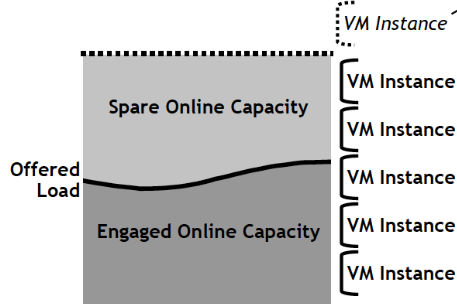
\includegraphics[width=.5\textwidth]{figures/cloud-spare-capacity.png}
  \end{center}
  \caption{Rappresentazione grafica semplificata della spare capacity}
  \label{fig:cloud-spare-capacity}
\end{figure}

Idealmente, le applicazioni dovrebbero prendere possesso della \textit{spare capacity} 
quando ne hanno bisogno (se possibile sottraendola anche a processi a bassa priorità).

Questo semplice meccanismo può realizzare una semplice forma di computing elastico. Quando
il carico aumenta la spare capacity diminuisce in quanto viene utilizzata da alcuni servizi. 
Quando l'utilizzo scende sotto una certa soglia, l'applicazione può ricostruire la spare 
capacity iniziale.

\paragraph{Slew rate} Quando bisogna attivare la spare capacity, le applicazioni fanno 
richiesta di avere nuove risorse, ma questo cambiamento non è istantaneo. L'intervallo di 
tempo in cui avviene questo processo decisionale definisce la latenza della risposta del 
sistema rispetto al cambiamento di input. Anche se questo è un concetto che origina dall'
elettroncia si parla di \textbf{\textit{slew rate}} quando si indica la velocità con cui 
varia l'uscita di un sistema quando varia l'input (Figura \ref{fig:cloud-slew-rate}).

\begin{figure}
  \begin{center}
    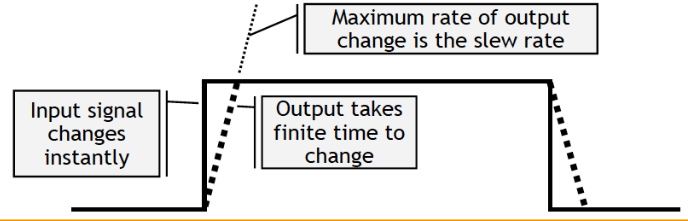
\includegraphics[width=.5\textwidth]{figures/cloud-slew-rate.png}
  \end{center}
  \caption{Definizione slew rate}
  \label{fig:cloud-slew-rate}
\end{figure}

Altri dettagli dello slew rate sono mostrati in Figura \ref{fig:cloud-slew-rate2}.
\begin{figure}
  \begin{center}
    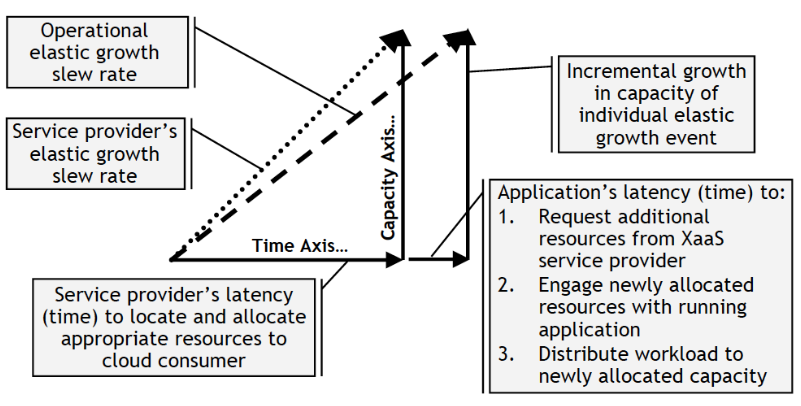
\includegraphics[width=.5\textwidth]{figures/cloud-slew-rate2.png}
  \end{center}
  \caption{Dettagli slew rate}
  \label{fig:cloud-slew-rate2}
\end{figure}

In un ambiente cloud \textit{XaaS} questo tempo di latenza è dovuto a: 

\begin{itemize}
  \item Richiedere le nuove risorse al cloud provider;
  \item Allocare le nuove risorse richieste per l'applicazione in esecuzione;
  \item Distribuire il workload sulle nuove risorse;
\end{itemize}

Questo tipo di approccio è molto complicato da implementare in quanto è possibile che non 
sempre siano disponibili ulteriori risorse da stanziare.

\paragraph{Capacity management}
Il processo di gestione della \textit{capacity} è riassunto in Figura 
\ref{fig:cloud-cap-management}.

\begin{figure}
  \begin{center}
    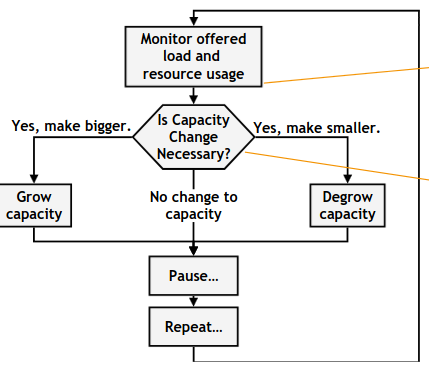
\includegraphics[width=.5\textwidth]{figures/cloud-cap-management.png}
  \end{center}
  \caption{Processo di gestione della capacity}
  \label{fig:cloud-cap-management}
\end{figure}

Sebbene virtualmente le applicazioni di un'infrastruttura cloud non possano mai soffrire di 
overload, si è visto che in realtà esistono modalità di \textbf{\textit{elasticity failure}}
(Figura \ref{fig:cloud-elasticity-failure}) in cui non si riesce ad allocare risorse allo 
stesso \textit{rate} con cui arrivano richieste. Inoltre, le applicazioni cloud sono 
soggette a latenza per tutta l'infrastruttura di monitoraggio e gestione delle risorse.

\begin{figure}
  \begin{center}
    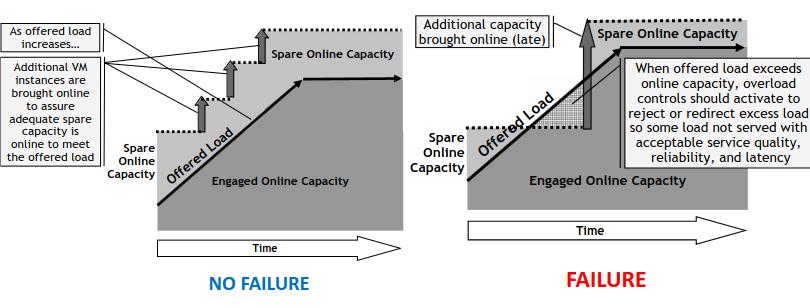
\includegraphics[width=.7\textwidth]{figures/cloud-elasticity-failure.png}
  \end{center}
  \caption{Esempio di elasticity failure}
  \label{fig:cloud-elasticity-failure}
\end{figure}

\clearpage
\section{Caratterizzazione di un workload}
Creare un workload sintetico rappresentativo di quello reale è fondamentale per l'analisi
delle performance di un sistema. A tal proposito, gli strumenti più utilizzati fanno parte
della statistica inferenziale il cui scopo principale è trarre informazioni su una 
popolazione avendo a disposizione solo sottoinsiemi ristretti di essa (campioni). Lo scopo
di questa parte del corso è quella di fornire modelli statistici per descrivere con un errore 
misurabile un workload reale, mantenendo i benefici di quello sintetico quali la 
replicabilità, semplicità di riproduzione, accuratezza \dots.


In quest'ambito, si definisce \textbf{SUT - System Under Test} come l'intero sistema sotto esame,
ma di solito si studiano sottosistemi che vengono \textbf{CUS - Component Under Test}.

\subsection{Richiami variabili aleatorie}

\subsubsection{Normalizzazione}
Il processo di normalizzazione dei dati significa applicare delle operazioni di scalatura
in modo tale da poter operare con i valori relativi. 

\paragraph{Z-score} La tecnica principale è quello dello \textit{z-score} che consiste 
nel trasformare il dataset iniziale, formato da $m$ parametri $\{x_{1k}, x_{2k}\dots x_{mk}
\}$, in uno di uguale dimensione, ma con media nulla e varianza unitaria. Per il $k-esimo$ 
parametro bisogna applicare la relazione in Equazione \ref{eq:zscore}.
\begin{equation}
  x'{ik} = \displaystyle\frac{x_{ik} - \overline{x}_k}{s_k}
  \label{eq:zscore}
\end{equation}

Dove con $s_k$ e $\overline{x}_k$ si indicano rispettivamente la deviazione standard a la 
media della componente $k$.

\subsection{Modelli statistici di base}
\subsubsection{Media campionaria}
La media campionaria è il modello statistico più semplice in quanto racchiude in un solo 
numero, il valore medio, un riassunto di un parametro dopo $n$ osservazioni. 
$$\overline{x} = \frac{1}{n}\displaystyle\sum_{i=1}^{n}x_i$$

Le $n$ oseervazioni costituiscono \textbf{campione} (\textbf{\textit{sample}}) che viene 
selezionato da un'ipotetica \textbf{popolazione} (non è detto che questa esista). Nella 
statistica inferenziale, la popolazione viene modellata da una \textit{pdf} e, quindi
essendo una variabile aleatoria, il suo valore medio $\mu$ può essere stimato 
ragionevolmente da $\overline{x}$.

In questo campo, quando ci sono campioni con poche osservazioni $n < 20$. Si utilizzano i
\textit{dot diagram}. Le osservazioni vengono messe su un semplice diagramma.

\paragraph{Problemi della media campionaria}
La media campionaria non è sempre il modello giusto per caratterizzare un dataset. Infatti,
può essere condizionata da \textit{outliers} e dallo \textbf{\textit{skewness}} (asimmetria)
dei dati. Per questo motivo, esistono altri $2$ modelli utilizzati a volte al posto della 
media:
\begin{itemize}
  \item \textbf{mediana}: si ottiene ordinando le osservazioni in ordine crescente e
    prelevando l'elemento centrale.
  \item \textbf{moda}: si ottiene attraverso un istograma delle frequenze e 
    prelevando l'elemento con più occorrenze.
\end{itemize}

Un semplice modo per il calcolare lo \textit{skewness} di un parametro è il rapporto tra 
il valore massimo e quallo minimo. Maggiore sarà questo valore, più alto è il grado di 
asimmetria della componente. $$ skew = \frac{y_{max}}{y_{min}}$$

Anche sono più robusti rispetto agli outliers, spesso media, mediana e moda non sempre 
sono intercambiabili e non  sempre esiste la moda in un campione statistico. In Tabella 
\ref{tab:usecase_simple_models}, è riportata una panoramica su casi d'uso reali con il 
relativo modello da utilizzare. Inoltre, in Figura \ref{fig:mean_mode_median_differences},
sono mostrate le differenze dei $3$ indici a seconda della distribuzione. si noti che per 
la distribuzione normale i valori coincidono.

\begin{table}
  \begin{center}
    \begin{tabular}[c]{c|c|c}
      \hline
      \multicolumn{1}{c|}{\textbf{Tipo di dato richiesto}} & 
      \multicolumn{1}{c|}{\textbf{Esempio}} & 
      \multicolumn{1}{l}{\textbf{Modello}} \\
      \hline
      Categorico & Quale è la risorsa più utilizzata in un sistema? & Moda \\
      Somma & Tempo di interarrivo delle richieste & Media \\
      Distribuzione \textit{skewed} & Carico medio su un sistema & Mediana \\
      \hline
    \end{tabular}
    \caption{Panoramica su quali casi d'uso utilizzare media, moda e mediana}
    \label{tab:usecase_simple_models}
  \end{center}
\end{table}

\begin{figure}
  \begin{center}
    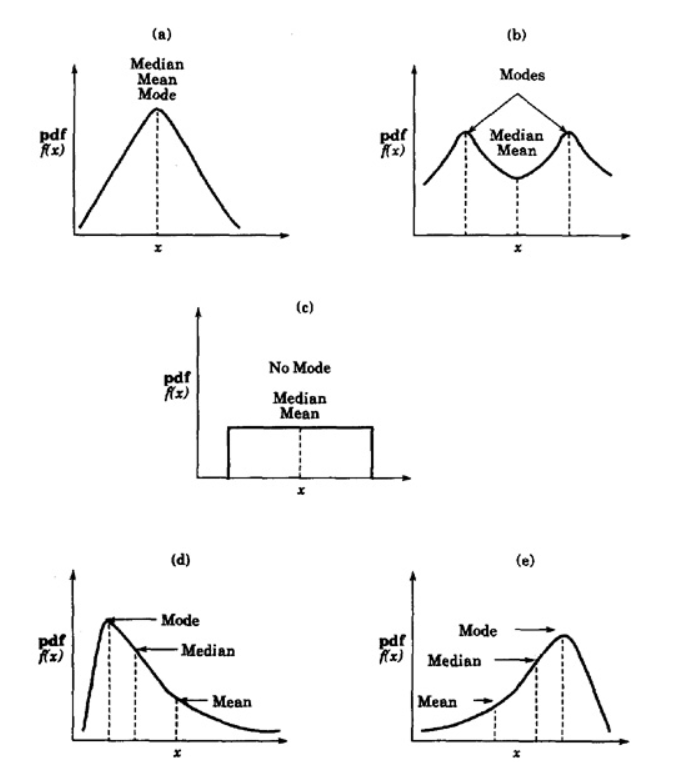
\includegraphics[width=.6\textwidth]{./figures/mode_mean_median.png}
  \end{center}
  \caption{Differenze tra moda, media e mediana in distribuzioni statistiche}
  \label{fig:mean_mode_median_differences}
\end{figure}


\subsubsection{Indici di dispersione}
La media, moda e mediana sono indici statistici semplici perchè racchiudono in una solo 
l'informazione generale di un dataset. Questo non basta per una caratterizzazione completa,
in quanto servono informazione non solo sui valori medi, ma anche sulla \textbf{variabilità}
di un dataset.
\paragraph{Varianza e devianza campionaria} La media non riesce ad esprimere tutte le informazioni sul campione iniziale. Per questo
motivo, si usano la \textbf{varianza campionaria} (\textbf{\textit{sample variance}},
Equazione \ref{eq:sample_variance}) e la \textbf{devianza campionaria} (\textbf{
  \textit{sample deviance}}. La devianza campionaria si esprime nella stessa unità di misura 
della grandezza misurata.

\begin{equation}
  s^2 = \displaystyle\frac{\displaystyle\sum_{i=1}^{n}(x_i - \overline{x})^2}{n-1}
  \label{eq:sample_variance}
\end{equation}

Analogamente alla media campionaria, questi due indici stimano, assumendo la popolazione 
iniziale come una variabile aleatoria descritta da una \textit{pdf}, la \textbf{varianza
($\sigma^2$}, Equazione) e la \textbf{deviazione standard ($\sigma$)}.

Si noti che in queste relazioni si divide sempre per $n-1$ (dove in questo caso $n-1$ sono
i gradi di libertà a disposizione). Infatti, si nota facilmente che la somma di tutte 
le devianze è nulla. Quindi dati $n-1$ valori della devianza, l'$n-esimo$ è automaticamente
definito.
\begin{equation*}
  x_1 - \overline{x} + x_2 - \overline{x} + \dots + x_n - \overline{x} = 0
\end{equation*}

\paragraph{Range del campione} Un indice facile da calcolare, a differnza della varianza campionaria, è il range. 
Semplicemente definito come in Equazione \ref{eq:sample_range}, aumenta all'aumentare della 
variabilità dei dati, ma ignora tutta la parte centrale dei dati. Analogamente alla media,
quest'indice è fortemente affetto dagli \textit{outlier}.

\begin{equation}
  r = \max(x_i) - \min(x_i)
  \label{eq:sample_range}
\end{equation}

In generale, non ha senso utilizzare questo indice a meno che non si è certi dell'ipotesi 
che i dati siano limitati (sia superiormente che inferiormente). 

\paragraph{Percentile}
I percentili dividono la distribuzione iniziale in $100$ parti. Supposte le osservazioni 
ordinate in maniera crescente, un valore $x$ si trova al $n\%$ se approssimativamente 
$n\%$ dei punti del dataset sono minori di $x$. Il valore che la $CDF$ assume in corrispondenza
di $x$ è detto $\alpha-Quantile$. Un'$\alpha-Quantile$ può essere ottenuto prendendo 
dalla distribuzione iniziale l'elemento in posizione $[(n-1)\alpha + 1]$.

\paragraph{Esempio} Data la sequenza $\{1.9,2.7,2.8,2.8,2.8,2.9,3.0,3.1,3.1,3.2,3.2\}$,
trovare il valore del $10\%$ percentile e dello $0.5-quantile$.

Sapendo che $n=11$, si applica la definizione trovando $0.1q = 10\% = v[10\cdot0.1 +1] = v[2] 
= 2.7$.

Sapendo che $n=11$, si applica la definizione trovando $0.5q = 50\% = v[10\cdot0.5 +1] = v[6]
= 2.9$.

\paragraph{Quartili} Con la definizione quantile si definiscono $3$ punti che dividono il 
dataset in $4$ parti:
\begin{itemize}
  \item \textbf{$Q_1$}: $25\%$ percentile;
  \item \textbf{$Q_2$}: $50\%$ percentile;
  \item \textbf{$Q_3$}: $75\%$ percentile;
\end{itemize}

Detti questi punti, si definisce il \textbf{\textit{semi inter-quartile range}} come 
descritto nella Equazione \ref{eq:siqr_def}.

\begin{equation}
  SIQR = \frac{Q_3 - Q_1} {2} = \frac{x_{0.75} - x_{0.25}} {2}
  \label{eq:siqr_def}
\end{equation}

\paragraph{Quantile-Quantile plot} Un plot quantile-quantile è sufficientemente robusto 
per determinare per via grafica se $2$ dataset appartengono a popolazioni con la stessa 
distribuzione. All'interno del corso, si usa questo grafico per verificare la normalità dei 
dati. Il plot quantile-quantile è fatto da una retta in cui i punti $x_i$\footnote{Per 
determinare i punti quantili di una distribuzione nota bisogna invertire la $CDF$. Quindi
$x_i = F^{-1}(q_i)$.} sono i quantili della distribuzione di riferimento (al quantile $q_{i}$
); mentre $y_i$ sono i punti del data set da studiare. 

In Figura \ref{fig:qqplots}, sono mostrati esempi di Quantile-Quantile plot. 

\begin{figure}
  \begin{center}
    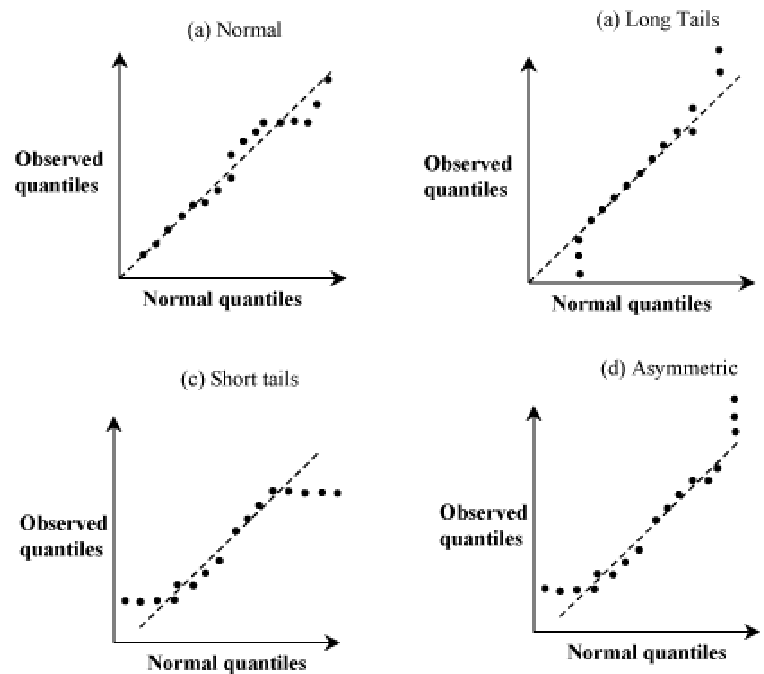
\includegraphics[width=.6\textwidth]{figures/qqplots.png}
  \end{center}
  \caption{Esempi di QQ-Plot in cui si confrontano i quantili di una distribuzione normale 
  con quelli di dataset osservati}\label{fig:qqplots}
\end{figure}


\subsubsection{Analisi grafica}
Talvolta, una rappresentazione grafica dei dati può essere utile per comprendere come si
comportano campioni con molte osservazioni.

\paragraph{Istogramma con singolo parametro} Con questo tipo di grafico (Figura 
\ref{fig:sp_histogram.png}) ci si concentra sulla frequenaza di un particolare parametro.
In particolare, l'analisi grafica mette in risalto la varianza facilmente 
identificabile dall'altezza delle colonne, ma trascura la correlazione.

\begin{figure}
  \begin{center}
    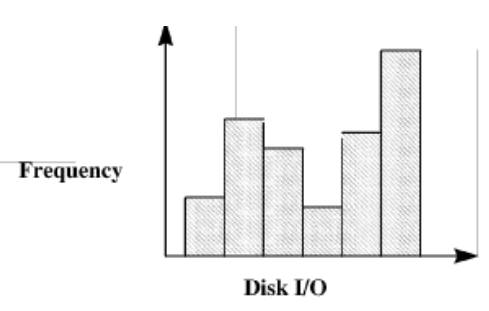
\includegraphics[width=.6\textwidth]{figures/sp_histogram.png}
  \end{center}
  \caption{Esempio di istogramma a singolo parametro}\label{fig:sp_histogram.png}
\end{figure}

\paragraph{Scatter plot} 
TODO

\subsection{PCA - Principal Component Analysis}
La \textit{PCA} è una trasformaziona lineare che prende il dataset iniziale e lo trasforma 
in uno in cui ogni componente è incorrelato dagli altri. In Equazione \ref{eq:weighted_sum},
è mostrata la definizione di componente principale $y_j$:
\begin{equation}
  y_j = \displaystyle\sum_{i=1}^{n} w_{ij} x_{ij}
  \label{eq:weighted_sum}
\end{equation}
Il risultato dell'analisi a componenti principali è un dataset delle stesse dimensioni di 
quello iniziale, ma le componenti principali esprimono in maniera decrescente la varianza 
dei dati (Figura \ref{fig:pca_outcame}). 
\begin{figure}
  \begin{center}
    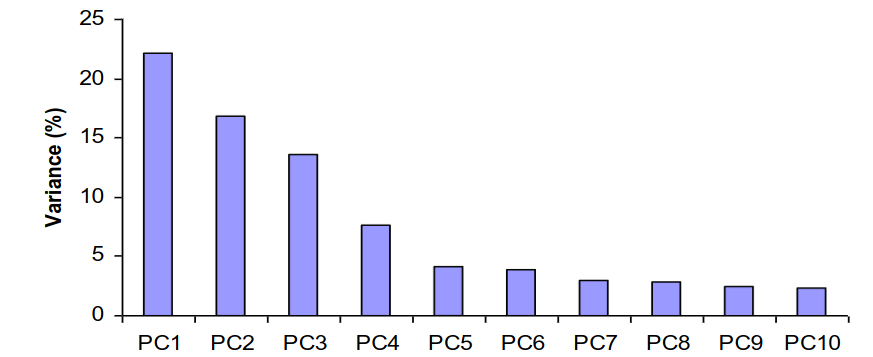
\includegraphics[width=.6\textwidth]{figures/pca_example.png}
  \end{center}
  \caption{Esempio: 10 componenti principali}\label{fig:pca_outcame}
\end{figure}

Il problema principale della trasformazione è quello di trovare i pesi $w_{ij}$.

Si dimostra che i pesi $w_{ij}$ sono gli autovettori che si ottengono applicando una 
trasformazione  di stato usando la matrice di correlazione (o covarianza)
\footnote{Si può prendere in maniera indipendente la matrice di correlazione covarianza 
poichè si assume (ragionevolmente) che nei sistemi di elaborazione i parametri analizzati 
sono sempre correlati linearmente.}. Di seguito sono mostrati i passi per eseguire questa 
trasformazione:
\begin{enumerate}
  \item Applicare la normalizzazione (\textbf{z-score}) al dataset;
  \item Calcolare $\overline{x}$ e $s$ per ogni componente;
  \item Calcolare la matrice di correlazione $C$;
  \item Usare $C$ per trovare gli autovalori $\lambda_i$ del sistema;
  \item Trovare gli autovettori del sistema $u_i$ scegliendo quelli di modulo unitario;
\end{enumerate}

In Equazione \ref{eq:correlation}, è mostrato come calcolare la matrice di correlazione 
per 2 componenti $x_s$ e $x_r$.

\begin{equation}
  R_{x_s,x_r} = \displaystyle\frac{\frac{1}{n} \sum_{i=1}^{n} (x_{si} -\overline{x}_s)(x_{ri} -\overline{x}_r)}{s_{x_s}s_{x_r}}
  \label{eq:correlation} 
\end{equation}

L'effetto della PCA è quello di proiettare i punti iniziali del dataset su un riferimento 
diverso racchiudendo la maggior parte varianza in poche componenti. Ad esempio, in Figura 
\ref{fig:2pc_plot}, si vede che la maggior parte della varianza è espressa da \textit{
  Principal factor 1}. Quindi nella caratterizzazione del workload possiamo trascurare 
lo studio della componente principale $2$ in quanto esprima poca varianza iniziale. In 
questo senso, si dice che si è applicato una \textbf{\textit{dimensionality reduction}}
che può semplicare studi futuri.

\begin{figure}
  \begin{center}
    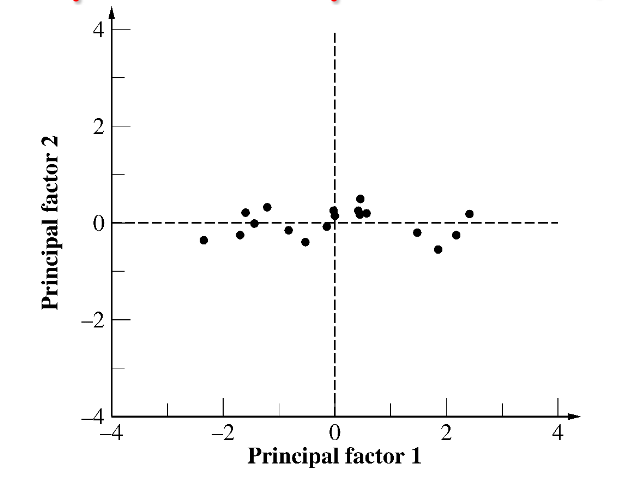
\includegraphics[width=.6\textwidth]{figures/2pc_plot.png}
  \end{center}
  \caption{Esempio 2 componenti principali}\label{fig:2pc_plot}
\end{figure}

Le componenti principali ottenute hanno media nulla. La percentuale di varianza mantenuta 
può essere calcolata effettuando la somma dei quadrati di ciascuna e rapportandola alla 
varianza totale per avere il valore percentuale.

Lo svantaggio principale (come si nota in Figura) è dato dal fatto che le componenti 
principali non alcun significato fisico e quindi non è possibile effettuare analisi 
qualitative sui dati ottentuti.

\begin{figure}
  \begin{center}
    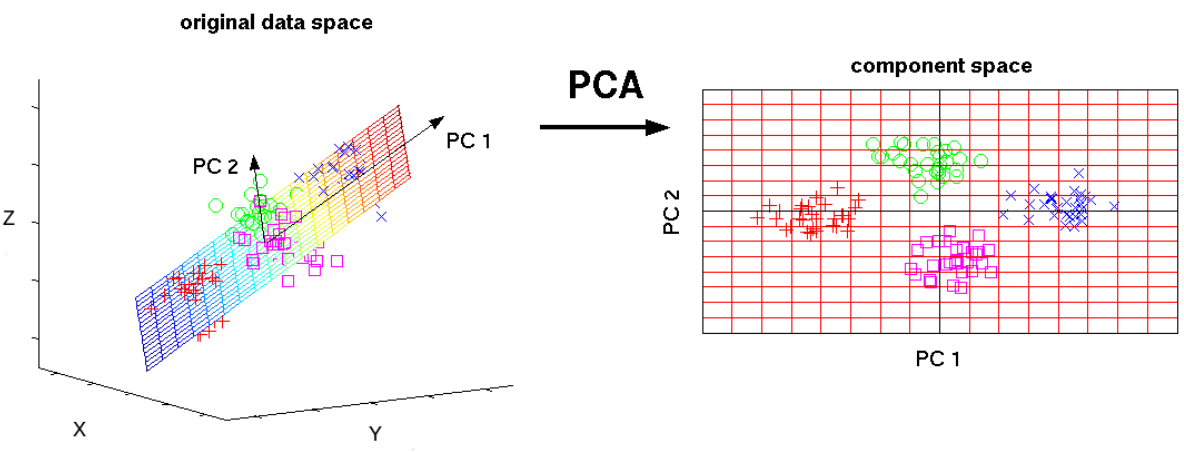
\includegraphics[width=.7\textwidth]{figures/pca_resultspace.png}
  \end{center}
  \caption{Esempio spazio risultato con due componenti principali}
\end{figure}

\clearpage
\subsection{Clustering}
All'interno delle analisi di prestazioni, il clustering può essere utile per dividere 
il dataset in classi per ognuna delle quali selezionare un elemento rappresentativo. 
Il problema principale del clustering è il criterio secondo cui due punti del dataset 
sono simili o dissimili. Di seguito sono riportate alcune strategie per determinare
l'elemento più rappresentativo di un cluster di punti.

\paragraph{Scelta randomica} Una possibile scelta è quella randomica. In questo modo, 
si perdono tutte le caratteristiche all'interno del cluster. Infatti è possibile che il 
punto scelto sia quello meno frequente nel cluster (un \textit{outlier}). 

\paragraph{Elemento più frequente} Laddove ha senso, è possibile contare le occorrenze di 
un punto con particolari proprietà all'interno del cluster.

\paragraph{Centroide} Il centroide di un cluster è l'elemento che ha il valore medio del 
cluster. Formalmente, dato un cluster $k$ di $n_k$ elementi, il suo centroide $\overline{X}
_k$ è definito come in Equazione \ref{eq:centroid}. Dove con la funzione $C(i) = k$ si 
includono solo gli elementi del cluster $k$.
\begin{equation}
  \overline{X}_k = \frac{1}{n_k} \displaystyle\sum_{C(i) = k} X_i
  \label{eq:centroid}
\end{equation}

In particolare, lo scopo del clustering è quello di partizionare le componenti di un dataset
in gruppi in modo tale da racchiudere in solo gruppo elementi simili tra loro. Dal punto di 
vista statistico, ciò significa minimizzare la varianza intra-cluster e massimizzare quella 
inter-cluster. Dato che la varianza di un dataset è costante, il suo centroide \begin{equation}
  var_{tot} = var_{intra} + var_{inter}
\end{equation}
Ciò significa che aumentando la varianza intra-cluster inevitabilmente si diminuisce la
inter-cluster.

\paragraph{Devianza intra-cluster} Formalmente, dati $K$ cluster con $n_k$ elementi ciascuno 
e centroide $\overline{X}_k$, detto $\overline{X}$ il valore medio del dataset, 
la devianza inter-cluster è definita secondo l'Equazione \ref{eq:intra-cluster_dev}.

\begin{equation}
  Dev_{intra} = \displaystyle\sum_{k=1}^{K} \displaystyle\sum_{C(i) = k}  
  ||\overline{X}_i - \overline{X}_k||^2 
  \label{eq:intra-cluster_dev}
\end{equation}
La devianza intra-cluster si definisce come la somma quadratica della distanza degli ogni 
elemento di un cluster dal centroide.

\paragraph{Devianza inter-cluster} Formalmente, dati $K$ cluster con $n_k$ elementi ciascuno 
e centroide $\overline{X}_k$, detto $\overline{X}$ il valore medio del dataset, 
la devianza inter-cluster è definita secondo l'Equazione \ref{eq:inter-cluster_dev}.

\begin{equation}
  Dev_{inter} = \displaystyle\sum_{k=1}^{K} n_k ||\overline{X}_k - \overline{X}||^2 
  \label{eq:inter-cluster_dev}
\end{equation}
La devianza inter-cluster si definisce come la distanza dei singoli centroidi con la media 
del dataset iniziale pesata per il numero degli elementi del cluster.

\paragraph{Metrica di distanza} Un problema di clustering consiste nel determinare i punti 
più vicini in uno spazio $n-dimensionale$. Per determinare la vicinanza si utilizzano delle
metriche (le più importanti sono riportate in Tabella \ref{tab:distance_metrics}. 

\begin{table}
  \begin{center}
    \begin{tabular}{ |l|c| } 
      \hline
      Euclidea & $\sqrt{\sum_{k=1}^{n}(x_{ik} - x_{jk})^2}$ \\ [1ex]
      \hline
      Euclidea pesata & $\sqrt{\sum_{k=1}^{n}w_{ij}(x_{ik} - x_{jk})^2}$ \\ [1ex]
      \hline
      Euclidea al quadrato & $\sum_{k=1}^{n}(x_{ik} - x_{jk})^2$ \\
      \hline 
    \end{tabular}
    \caption{Riassunto metriche di distanza più utilizzate}
    \label{tab:distance_metrics}
  \end{center}
\end{table}

La metrica euclidea al quadrato è molto usata per determinare la distanza tra cluster perchè
simile alla devianza, ma non rispetta la proprietà di disuguaglianza triangolare. 
Quella pesata, invece, si applica quando non è stata effettuata in precedenza la 
normalizzazione dei dati. In generale, la più utilizzata resta la quella euclidea.

\paragraph{Tecniche di cluster} Nel corso è mostrata la tecnica di clustering gerarchico. 
Questa può essere effettuata in due modi:
\begin{itemize}
  \item \textbf{Agglomerativo}: inizialemente ogni elemento costituisce un cluster. Ad ogni
    iterazione, i cluster più vicino vengono fusi tenendo traccia di una matrice delle 
    distanze fino ad ottenere un solo cluster con tutti gli elementi;
  \item \textbf{Divisivo}: tutti gli elementi vengono posti inizialmente in un singolo 
    cluster e successvimente viene effettuata una divisione fino ad ottenere gruppi 
    formati da singoli elementi;
\end{itemize}

\subsubsection{Clustering gerarchico e agglomerativo}
Il clustering gerarchico agglomerativo visto al corso prevede l'utilizzo del metodo di Ward 
per minimizzare la varianza all'interno di un cluster. Questo metodo fa parte di una famiglia
di strategie basate sullo studio della varianza che si contrappongono a quelli basati sulla
distanza euclidea.

\paragraph{Single Linkage Clustering} In questa strategia, la distanza tra due cluster 
è la minimima distanza tra due punti appartenenti ai due gruppi (Figura 
\ref{fig:cl-single_linkage}). Formalmente, dati due cluster $P, Q$, $x \in P$ e $y \in Q$, 
allora la distanza tra $P$ e $Q$ è:
$$d(P,Q) = \min {d(x,y)}$$

\begin{figure}
  \begin{center}
    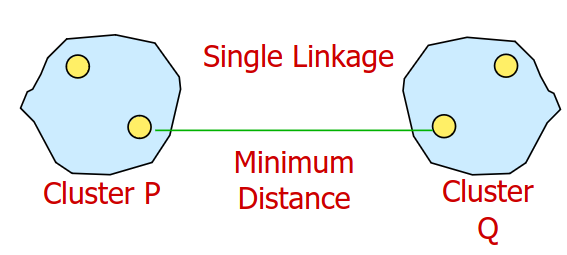
\includegraphics[width=0.65\textwidth]{figures/cl-single_linkage.png}
  \end{center}
  \caption{Esempio single linkage clustering}\label{fig:cl-single_linkage}
\end{figure}


\paragraph{Complete Linkage Clustering} In questa strategia, la distanza tra due cluster 
è la massima distanza tra due punti appartenenti ai due gruppi (Figura 
\ref{fig:cl-complete_linkage}). Formalmente, dati due cluster $P, Q$, $x \in P$ e $y \in Q$, 
allora la distanza tra $P$ e $Q$ è:
$$d(P,Q) = \max {d(x,y)}$$

\begin{figure}
  \begin{center}
    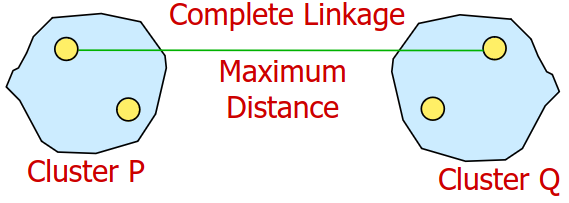
\includegraphics[width=0.65\textwidth]{figures/cl-complete_linkage.png}
  \end{center}
  \caption{Esempio complete linkage clustering}\label{fig:cl-complete_linkage}
\end{figure}

\paragraph{Average Linkage Clustering} In questa strategia, la distanza tra due cluster 
è la massima distanza tra due punti appartenenti ai due gruppi (Figura 
\ref{fig:cl-average_linkage}). Formalmente, dati due cluster $P, Q$, $x \in P$ e $y \in Q$, 
allora la distanza tra $P$ e $Q$ è:
$$d(P,Q) = mean\; d(x,y)$$

\begin{figure}
  \begin{center}
    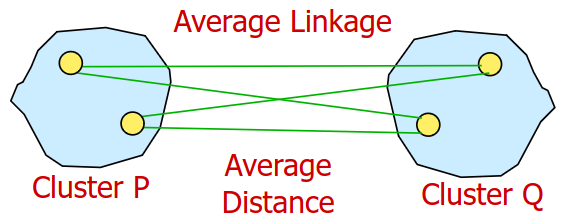
\includegraphics[width=0.65\textwidth]{figures/cl-average_linkage.png}
  \end{center}
  \caption{Esempio average linkage clustering}\label{fig:cl-average_linkage}
\end{figure}

\paragraph{Metodo dei centrodi} In questa strategia, la distanza tra due cluster 
è calcolata a partire dai centroidi(Figura\ref{fig:cl-centroid_method}). Formalmente, dati 
due cluster $P, Q$, $x \in P$ e $y \in Q$, allora la distanza tra $P$ e $Q$ è:

$$d(P,Q) = || \overline{x}_P - \overline{x}_Q||$$

\begin{figure}
  \begin{center}
    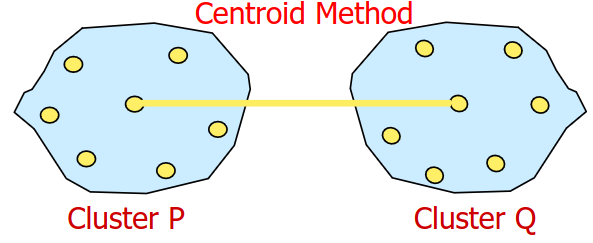
\includegraphics[width=0.65\textwidth]{figures/cl-centroid_method.png}
  \end{center}
  \caption{Esempio di utilizzo del metodo dei centrodi}\label{fig:cl-centroid_method}
\end{figure}

\paragraph{Metodo di Ward} In questa strategia, la distanza tra due cluster 
è calcolata a partire dai centroidi(Figura 
\ref{fig:cl-ward_method}). Formalmente, dati due cluster $P, Q$, $x \in P$ e $y \in Q$, 
allora la distanza tra $P$ e $Q$ è:
$$d(P,Q) = 2 \displaystyle\frac{|P| |Q|}{|P| + |Q|} || \overline{x}_p - \overline{x}_q||^2$$

In cui con $|P|$ e $|Q|$ si è indicato il numero di elementi del cluster $P$ e $Q$; mentre 
con $\overline{x}_P$ e $\overline{x}_Q$ i centroidi di $P$ e $Q$. Si noti che la distanza di 
Ward è la distanza euclidea al quadrato pesata per le dimensioni dei cluster in questione.
\begin{figure}
  \begin{center}
    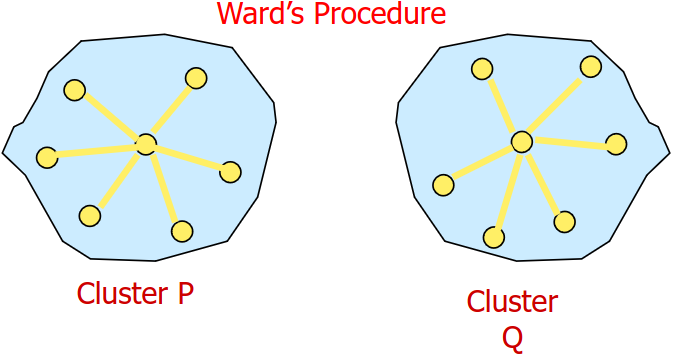
\includegraphics[width=0.65\textwidth]{figures/cl-ward_method.png}
  \end{center}
  \caption{Esempio di utilizzo del metodo di Ward}\label{fig:cl-ward_method}
\end{figure}

\clearpage
\subsection{Statistica inferenziale}
La statistica inferenziale ha come obiettivo quello di caratterizzare una popolazione a 
partire da campioni. In particolare, si compone di due parti:
\begin{enumerate}
  \item Stima dei parametri;
  \item Test di ipotesi;
\end{enumerate}

\subsubsection{Stima dei parametri}
Si parta da un \textbf{campione} (\textbf{\textit{sample}}) di $n$ \textbf{osservazioni}. 
Prima di effettuare le $n$ osservazioni, ciascuna di queste è considerata essere una 
variabile aleatoria $X_1, X_2, \dots, X_n$. Quindi, qualsiasi funzione\footnote{Una funzione
applicata su una variabile aleatoria è anche detta \textbf{statistica}.} si applica a queste
osservazioni risulta essere anch'essa una variabile aletoria e, pertanto, avrà una 
distribuzione di probabilità (\textbf{pdf}) che sarà detta \textbf{\textit{sampling
distribution}}. 

Detto $\theta$ il parametro da stimare (può essere $\mu$ o $\sigma^2$), si dice che $\hat{
  \theta} = h(X_1, X_2, \dots, X_n)$ è un estimatore del parametro $\theta$ ed è anch'esso
una variabile aleatoria.

\paragraph{Teorema del limite centrale}
Si dice che l'insieme delle variabili aleatorie $X_1, X_2, \dots, X_n$ sono un campione 
randomico (\textbf{\textit{random sample}}) se e solo se:

\begin{enumerate}[label=(\alph*)]
  \item $X_i\;\forall i = 1\dots n$ sono variabli aleatorie indipendenti tra loro;
  \item $X_i\;\forall i = 1\dots n$ ha la stessa distribuzione di probabilità;
\end{enumerate}

Definito il \textit{random sampling}, il teorema del limite centrale afferma che: 
dato un \textit{random sample} $X_1, X_2, \dots, X_n$ di grandezza $n$ preso da una 
popolazione con media $\mu$ e varianza $\sigma^2$ e,  detta $\overline{X}$ la media 
campionaria, la distribuzione ottenuta in Eqauzione \ref{eq:th-central_limit}.
\begin{equation}
  Z = \displaystyle\frac{\overline{X} - \mu}{\sigma/\sqrt{n}}
  \label{eq:th-central_limit}
\end{equation}

tende alla distribuzione normale per $n\rightarrow \infty$. Nella pratica, il teorema del 
limite centrale vale per $n \geq 30$.
\paragraph{Intervallo di confidenza}
Formalmente, una stima di un intervallo di confidenza per $\mu$ è specificato nella forma 
$l \leq \mu \leq u$. In particolare, essendo $l$ e $u$ ricavati da campioni della popolazione
iniziale, allora questi costituiscono variabili aleatorie $L$ e $U$. Si vogliono determinare
$L$ e $U$ tale che sia vero il predicato:
$$ P\{L\leq \mu \leq U\} = 1 - \alpha $$

Dove con $l$ e $u$ si indicano rispettivamente il limite inferiore e superiore di confidenza
e con $\alpha$ si indica il coefficiente di confidenza.Sotto del teorema del limite
centrale (Equazione \ref{eq:th-central_limit}, e distribuzione normale),
si possono determinare questi fattori com segue:

\begin{align*}
  P\{l\leq \mu \leq l\} = 1 - \alpha  \\
  P\{-z_{\alpha/2} \leq \displaystyle\frac{\overline{X} -\mu}{\sigma/\sqrt{n}} 
  \leq z_{\alpha/2} \} = 1 - \alpha  \\
  P\{-\frac{\sqrt{n}}{\sigma}z_{\alpha/2} \leq \overline{X} -\mu \leq \frac{\sqrt{n}}
  {\sigma} z_{\alpha/2}\} = 1 - \alpha \\
  P\{\overline{X} -\frac{\sqrt{n}}{\sigma}z_{\alpha/2} \leq \mu \leq \overline{X} +\frac{\sqrt{n}}
  {\sigma} z_{\alpha/2}\} = 1 - \alpha
\end{align*}

In cui $z_{\alpha/2}$ è il percentile $100\alpha/2$ della distribuzione normale.

L'intevallo di confidenza al $95\%$ non significa che esiste una probabilità del $95\%$ che 
il parametro $\hat{\theta}$ stimato si trovi nel range di valori trovato. Il parametro 
della popolazione è sconosciuto e, per come si è definito l'intervallo di confidenza 
si basa su $L$ e $U$ che sono variabili aleatorie. L'interpretazione corretta di un intervallo
di confidenza di $100(1-\alpha)\%$ è che se un numero infinito di di intervalli di confidenza
viene calcolato per il parametro $\mu$, allora il $100(1-\alpha)\%$ di questi intervalli 
contiene il valore reale di $\mu$.

\paragraph{Scelta della dimensione del campione $n$}
Stimando il valore di un parametro di una distribuzione con fattori ottenuti da variabili
aleatorie si commette un errore. In particolare, si definisce l'\textbf{errore standard}
(\textbf{\textit{standard error}}) come la differenza tra la stima e il valore reale: 
$$ E = |\overline{x} - \mu | $$
Quindi usando un CI del $100(1-\alpha)\%$, l'errore totale $(2E)$ che si puo commettere è pari alla
lunghezza dell'intervallo, asserendo quindi che $E = z_{\alpha/2}\sigma\sqrt{n}$.

Detto questo, come mostrato in Equazione \ref{eq:sample-size}, 
si può agire su $n$ per essere sicuri che l'errore sia commesso sia minore un certo limite 
$E$.

\begin{equation}
  n = \left(\displaystyle\frac{z_{\alpha/2} \sigma}{E}\right)^2
  \label{eq:sample-size}
\end{equation}
Il risultato dell'Equazione \ref{eq:sample-size} deve essere arrotondato per eccesso al 
fine di garantire che la confidenza non cada sotto il $100(1-\alpha)\%$.

\paragraph{Intervallo di confidenza per $\mu$ senza teorema del limite centrale}
I valori per l'intervallo di confidenza visti in precedenza valgono sotto l'ipotesi del 
teorema del limite centrale: popolazione è normale con media sconosciuta $\mu$ e deviazione 
standard sconosciuta $\sigma$. Se la distribuzione non è quella normale, ma si conosce la 
varianza $\sigma^2$, si può usare la forma generalizzata dell'intervallo di confidenza 
presentata in Equazione \ref{eq:large_sample-confidence_interval}. A differenza del teorema
del limite centrale, la relazione vale per $n \geq 40$.

\begin{equation}
  \overline{x} - z_{\alpha/2}\frac{s}{\sqrt{n}} \leq \mu \leq \overline{x} + z_{\alpha/2}\frac{s}{\sqrt{n}}
  \label{eq:large_sample-confidence_interval}
\end{equation}

Dove si assume per $n \geq 40$ che la quantità in Equazione \ref{eq:approx-normal} segue
approssimativamente una distribuzione normale.

\begin{equation}
  \displaystyle\frac{\overline{X} - \mu}{S/\sqrt{n}} 
  \label{eq:approx-normal}
\end{equation}

Si noti come è stato approssimato la $S$ dell'Equazione \ref{eq:approx-normal} (deviazione
standard della popolazione) con la $s$ (deviazione standard del campione) della 
\ref{eq:large_sample-confidence_interval} commettendo un ulteriore errore che sarà mitigato 
dalla scelta $n \geq 40$. 

\paragraph{Intervallo di confidenza per $\mu$ con distribuzione normale e varianza 
sconosciuta}
Quando non si riesce ad avere $n \geq 40$, non si può usare l'intervallo di confidenza
definito in Equazione \ref{eq:large_sample-confidence_interval}, ma bisogna usare la 
distribuzione $t$. Quindi dato un campione randomico $X_1, X_2, \dots, X_n$ da una 
distribuzione normale con media $\mu$ e varianza $\sigma^2$ sconosciuti, allora la 
variabile aleatoria in Equazione \ref{eq:t-distribution}  ha una distribuzione $t$ con $n-1$
gradi di libertà.

\begin{equation}
  T = \displaystyle\frac{\overline{X} - \mu}{S\sqrt{n}}
  \label{eq:t-distribution}
\end{equation}

La $pdf$ della distribuzione $t$ è mostrata in Equazione \ref{eq:t-distribution-pdf} 
(Figura \ref{fig:t-distribution}).

\begin{equation}
  f(x) = \displaystyle\frac{\Gamma[k+1]/2}{\sqrt{\pi k}\Gamma(k/2)} \cdot
  \displaystyle\frac{1}{[x^2/k] + 1^{(k+1)/2}}
  \label{eq:t-distribution-pdf}
\end{equation}

dove $k$ è il numero di gradi di libertà. Nella distribuzione $t$ la media è nulla la 
varianza è $k/(k-2)$.

\begin{figure}
  \begin{center}
    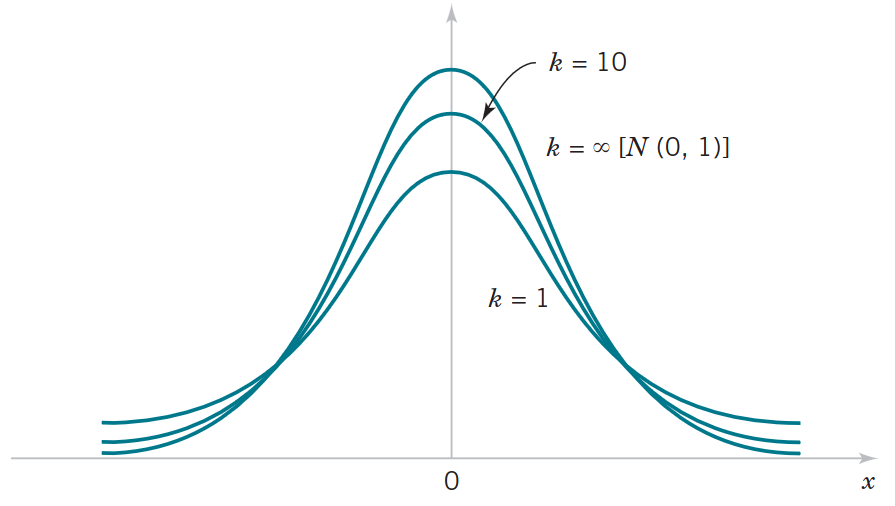
\includegraphics[width=.8\textwidth]{figures/t-distribution.png}
  \end{center}
  \caption{Funzioni di densità probabilità di alcune distribuzioni $t$ al variare di $k$}
  \label{fig:t-distribution}
\end{figure}

Definita la distribuzione $t$, è possibile definire un intervallo di confidenza similmente 
a quanto fatto in precedenza. Infatti, detta $\overline{x}$ la media di un random sample, 
si può stimare la $\mu$ di una popolazione normale con il $CI$ rappresentato in Equazione
\ref{eq:t-distribution-ci}. 

\begin{equation}
  \overline{x} - t_{\alpha/2,n-1} s\sqrt{n} \leq \mu \leq 
  \overline{x} + t_{\alpha/2,n-1} s\sqrt{n} 
  \label{eq:t-distribution-ci}
\end{equation}

dove $t_{\alpha/2,n-1}$ è il percentile $100\alpha/2$ della distribuzione $t$ con $n-1$ gradi
di libertà.

\subsubsection{Test di ipotesi}
Questa parte della statistica inferenziale si occupa di stabilire quale tra due affermazioni
o predicati circa un parametro risulta vero. I predicati sono chiamati \textbf{ipotesi} e la 
procedura utilizzata per prendere una decisione è detta \textbf{test di ipotesi}. Formalmente,
un'\textbf{ipotesi statistica} è un'affermazione sui di una o più popolazioni. Dato che la 
stima dei parametri è fatta a partire da variabili aleatorie un'ipotesi statistica può essere 
vista come un'affermazione sulla distribuzione di probabilità di una variabile aleatori
Ad esempio, si vuole decidere se è vero o meno che la media del tasso incendiario è
$50$ centimetri al secondo. Formalmente, ci sono due ipotesi:

\begin{enumerate}[label=(\alph*)]
  \item $H_0$: $\mu = 50$ centimetri al secondo;
  \item $H_1$: $\mu \neq 50$ centimetri al secondo;
\end{enumerate}

$H_0$ è detta \textbf{ipotesi nulla}; mentre $H_1$ è detta \textbf{ipotesi alternativa} e 
contraddice l'ipotesi nulla. In questo caso, si parla di \textbf{\textit{two sided 
alternative hypothesis}} perchè può essere o $\mu < 50$ o $\mu > 50$. Se invece, l'ipotesi 
alternativa fosse stata $\mu < 50$ (o il contrario) si sarebbe parlato di 
\textbf{\textit{one sided alternative hypothesis}}.
Supponendo che $48.5 \leq \overline{x} \leq 51.5$, l'ipotesi nulla $H_0$ non sarà rigettata,
ma questa sarà rigettata in favore di quella alternativa solo se o $\overline{x} \leq 48.5$
$\overline{x} \geq 51.5$. 

In questo caso, $\overline{x} = 48.5$ e $\overline{x} = 51.5$ sono detti \textbf{valori 
critici} (\textbf{\textit{critical values}}) e delimitano la regione critica $x < 48.5$ e 
$x > 51.5 $, mentre l'intervallo $48.5 \leq \overline{x} \leq 51.5$ è detto \textbf{regione
di accettazione} (\textbf{\textit{acceptance region}}).

\paragraph{Tipi di errore}
Dato che il calcolo di $\overline{x}$ dipende dal campione può succedere che il valore stimata
si trovi all'interno della regione critica quando il valore $\mu$ risulta essere proprio 
quello definito da $H_0$ in questo caso si sta commettendo un \textbf{errore di tipo I}. Al 
contrario, se $\overline{x}$ si trova all'interno della regione di accettazione, ma $\mu$ 
è all'esterno, l'ipotesi nulla non risulta rigettata quando dovrebbe. In questo caso di parla 
di \textbf{errore di tipo II}.

\paragraph{$\alpha-$error}
Visto che la decisione deriva da variabili aleatorie 
si parla di probabilità dell'errore. In particolare si calcola la probabilità dell'errore di 
tipo I $$\alpha = P(type\; I\; error)$$ ($\alpha$ è detto livello di significativia, $\alpha$ 
-error o grandezza del test).


Tornando all'esempio precedente, supposto $n = 10$ e $\sigma = 2.5$, si può calcolare $\alpha$ 
come:
\begin{equation*}
  \alpha = P(\overline{X} < 48.5\;quando\; \mu = 50) + P(\overline{X} > 51.5\;quando\; 
  \mu = 50)
\end{equation*}

Quindi sapendo che $\sigma / \sqrt{n} = 0.79$ si possono calcolare i valori \textit{z-score}:
\begin{align*}
  z_1 &= \displaystyle\frac{48.5-50}{0.79} = -1.90\\
  z_2 &= \displaystyle\frac{51.5-50}{0.79} = 1.90
\end{align*}
Si ottiene che:
\begin{equation*}
  \alpha = P(z < -1.90) + P(z > 1.90) = 0.0287 + 0.0287 = 0.0574 
\end{equation*}

Si noti che l'errore può essere diminuito aumentando la dimensione del campione $n$.
\paragraph{$\beta-$error}
Analogamente al $\alpha-$error, si definisce $\beta-$error come la probabilità che 
verifica un errore di tipo II:

$$\beta = P(type\; II\; error)$$

Come all'$\alpha-$error bisogna calcolarlo per specifici valori di $\mu$. Ad 
esempio, si vuole calcolare:

$$\beta = P(48.5 \leq \overline{X} \leq 51.5\; quando\; \mu = 52)$$

Con calcoli simili, si ottiene:

\begin{align*}
  z_1 &= \displaystyle\frac{48.5-52}{0.79} = -4.43\\
  z_2 &= \displaystyle\frac{51.5-52}{0.79} = -0.63
\end{align*}

Si ottiene che:

\begin{equation*}
  \alpha = P( -4.43 \leq Z \leq -0.63) = P(Z\leq -0.63) - P(Z\leq-4.43) = 0.2643 
\end{equation*}
Il $\beta-$value è aumenta quando ci si avvicina al valore ipotizzato e diminuisce all'
aumentare di $n$. Inoltre, viene anche usato per definire la \textbf{potenza} di un test 
statistico: la probabilità di rigettare l'ipotesi nulla $H_0$ quando l'ipotesi alternativa 
è vera. Si calcola come:
$$  power = 1 - \beta $$

\paragraph{P-Value}
Il P-Value è definito come il più piccolo livello di significatività che condurrebbe al 
rigetto dell'ipotesi nulla. In altre parole il P-Value indica la probabilità con cui ci 
si trova all'interno della regione critica (Figura \ref{fig:pvalue}). Nell'esempio precedente
, prendendo $n=16$, $\mu = 50$, $\sigma = 2.5$, si ottiene:
\begin{align*}
  P-Value &= 1 - P(48.7 < \overline{X} < 51.3) \\
  &= 1 - P\left(\displaystyle\frac{48.7 - 50}{2.5\sqrt{16}} < Z < \displaystyle\frac{
    51.3 - 50}{2.5\sqrt{16}}\right) \\
  &= 1 - 0.962 = 0.038
\end{align*}

\begin{figure}
  \begin{center}
    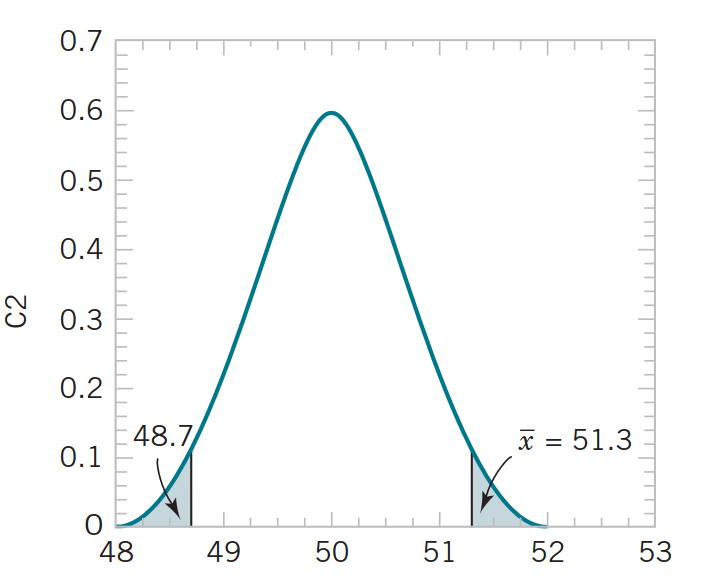
\includegraphics[width=.5\textwidth]{figures/pvalue}
  \end{center}
  \caption{Le aree evidenziate sono rappresentate dal P-Value}\label{fig:pvalue}
\end{figure}

\subsubsection{Zero mean test}
Si vuole usare un test di ipotesi per capire se la media di una popolazione corrisponde ad
un certo valore. Il test più semplice che si può effettuare è quello di verificare se la 
media stimata è nulla. Ciò può essere fatto controllando se l'intervallo di confidenza del 
valore stimato $\overline{x}$ include lo zero. Dal punto di vista statistico, si può 
applicare la definizione di $CI$:
\[
  \overline{x} - t_{\alpha/2,n-1}s/\sqrt{x} \leq \mu \leq 
  \overline{x} + t_{\alpha/2,n-1}s/\sqrt{x}
\]

\subsubsection{Comparare due alternative: \textbf{t-test}}
La maggior parte dell'analisi delle performance ha come scopo quello di comparare più sistemi
per capire quale è il migliore. Ammesso di aver estratto i campioni utilizzando workload 
comparabili si può effettuare un test simile a quello della media nulla per capire se i 
sistemi sono statisticamente significativi. In particolare, le procedure descritte di seguito
prendono il nome di \textbf{\textit{t-test}}.

\paragraph{Paired observation}Se si riescono a condurre $n$ esperimenti su ciascun sistema 
si dice che le osservazioni sono \textbf{\textit{paired}}. In questo caso per ogni coppia
di osservazioni si calcola la differenza su cui si calcola un intervallo di confidenza. 

Ad esempio, date le seguenti osservazioni $\{(5.4, 19.1), (16.6, 3.5), (0.6, 3.4), (1.4, 2.5)
(0.6, 3.6, 7.3, 1.7)\}$, si ha che $n = 6$, mentre la differenza delle osservazioni è
$\{-13.7, 13.1, -2.8, -3.0, 5.6\}$. Ottenuto questo campione, è possibile caratterizzarlo
con:
\begin{enumerate}[label=(\alph*)] 
  \item Media campionaria: $\overline{x} = -0.32$;
  \item Varianza campionaria $ S^2 = 81.62$;
  \item Deviazione standard campionaria $ S= 9.03$;
\end{enumerate}

Quindi trovato che $t_{0.95, 6-1} = 2.05$, si ottiene l'intervallo di confidenza:
\[
  -032 \mp (2.05)\frac{9.03}{\sqrt{81.62}} = (-7.75, 7.11)
\]

L'intevallo ottenuto contiene lo $0$ quindi i due sistemi da cui provengono le osservazioni
non sono statisticamente differenti.

\paragraph{Unpaired observation}Quando si hanno due campioni di dimensioni differenti, si 
dice che le osservazioni sono \textbf{\textit{unpaired}}. Detti $n_a$ e $n_b$ le dimensioni 
dei due campioni relativi ai due sistemi in esame $A$ e $B$, si eseguono i seguenti passi

\begin{enumerate}[label=(\alph*)] 
  \item Si calcolano la medie campionarie $\overline{x_a} = \frac{1}{n_a}\sum_{i=1}^{n_a}x_{ia}$ 
    e $\overline{x_b} = \frac{1}{n_b}\sum{i=1}^{n_b}x_{ib}$;
  \item Si calcolano le deviazioni standard campionarie 
    $s_a = \sqrt{\frac{\sum_{i=1}^{n_a}x_{ia}^2 - n_a\overline{x}^2_a}{n_a - 1}}$ e 
    $s_b = \sqrt{\frac{\sum_{i=1}^{n_b}x_{ib}^2 - n_b\overline{x}^2_b}{n_b- 1}}$;
  \item Si calcola la differenza media: $\overline{x} = \overline{x}_a - \overline{x}_b$;
  \item Si calcola la deviazione standard della differenza $s = \sqrt{\frac{s_a^2}{n_a} + 
    \frac{s_b^2}{n_b}}$;
  \item Si calcolano i gradi di libertà effettivi $\nu = \frac{(s_a^2/n_a + s_b^2/n_b)^2}
    {\frac{1}{n_a+1}(\frac{s_a^2}{n_a})^2 + \frac{1}{n_b + 1} (\frac{s_b^2}{n_b+1})^2 } - 2$;
  \item Si calcola l'intervallo di confidenza della differenza delle medie campionarie:
    $(\overline{x}_a - \overline{x_b}) \mp t_{[1-\alpha/2, \nu]} s$
\end{enumerate}

Analogamente al caso \textit{paired}, se l'intervallo contiene lo zero i due sistemi sono 
statisticamente equivalenti.
\subsubsection{Covarianza}
Un modo per capire se due variabili sono dipendenti è quello di osservare come covariano. 
Intuitivamente, la covarianza si nota quando una variabile si discosta dalla media produce
un effetto su un'altra variabile che varia dalla media nello stesso modo o nella stessa 
direzione o in maniera opposta. Formalmente la covarianza si esprime come lo scostamento
di due variabili dalla loro media (Equazione \ref{eq:covariance}), in maniera simile alla
varianza.
\begin{equation}
  Cov(x.y) = \frac{\displaystyle\sum_{i=1}^{n}(x_i - \overline{x})(y_i - \overline{y})}{n-1}
  \label{eq:covariance}
\end{equation}
Scritta così la covarianza non significa molto perchè è relativa alla scala della misura. 
L'Equazione \ref{eq:covariance}viene standardizzata attraverso il coefficiente di 
\textit{Pearson} mostrato in Equazione \ref{eq:covariance-pearson}.

\begin{equation}
  r =\frac{Cov(x.y)}{s_xs_y} =
  \frac{\displaystyle\sum_{i=1}^{n}(x_i - \overline{x})(y_i - \overline{y})}{(n-1)s_xs_y}
  \label{eq:covariance-pearson}
\end{equation}

Si dimostra che $-1 \leq r \leq 1$:
\begin{enumerate}[label=(\alph*)] 
  \item $r = 1$: le due variabili sono perfettamente correlate positivamente : se una aumenta
    anche l'altra aumenta di una quantità proporazionale;
  \item $r = 1$: le due variabili sono perfettamente correlate negativamente : se una aumenta 
    l'altra diminuisce di una quantità proporazionale;
\end{enumerate}

\clearpage
\subsection{Regressione lineare}
In statistica, si usa la regressione per ricavare modelli empirici che approssimano
l'andamento di dati ottenuti attraverso misurazioni dirette. Spesso, la relazione che si 
trova tra le variabili di un esperimento è non deterministica. Ad esempio, il consumo 
elettrico di una casa ($y$) dipende dalla grandezza della casa ($x$), ma non è una relazione
deterministica. In questo corso, si ipotizzano i parametri in una relazione lineare e, 
pertanto, si parla di regressione lineare (si utilizzano modelli lineari).

\paragraph{Utilizzo sbagliato della regressione} I modelli regressivi non devono essere
utilizzati per creare correlazioni di tipo causale tra i parametri dell'esperimento. 
Solo attraverso un \textbf{\textit{designed experiment}} è possibile determinare rapporti 
causa-effetto.\\

Il processo di analisi di variabili collegate in maniera non deterministica è detto 
\textbf{analisi di regressione}. La variabile $x$ è detta \textbf{predittore}, mentre $y$ è
detta \textbf{risposta}. In generale, si parte da uno \textit{scatter diagram} (Figura
\ref{fig:regression-scatter}) che rappresenta un insieme di $n$ coppie derivate 
da un'osservazione $(x_i, y_i)$ e si vuole creare un modello lineare:

$$ 
E(Y|x) = \beta_0 + \beta_1 x
$$

\begin{figure}
  \begin{center}
    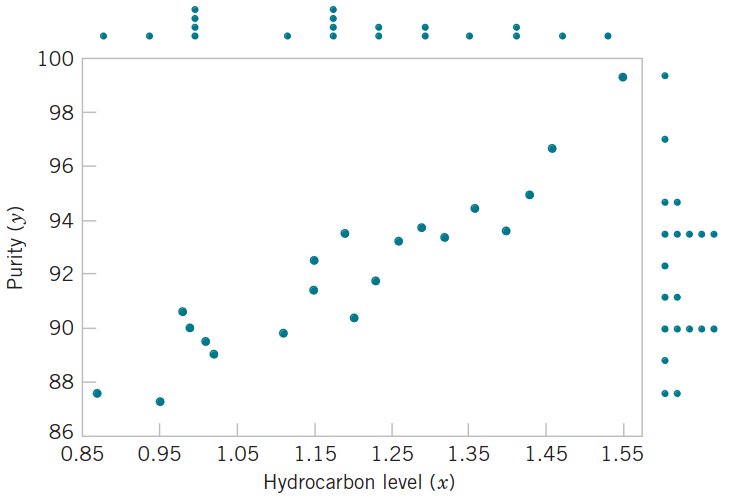
\includegraphics[width=0.8\textwidth]{figures/regression_scatter.png}
  \end{center}
  \caption{Esempio di scatter plot su cui effettuare l'analisi di regressione}
  \label{fig:regression-scatter}
\end{figure}

in cui il coefficiente angolare $\beta_1$ e l'intercetto $\beta_0$ sono detti 
\textbf{coefficienti di regressione}. In particolare, si assume che ogni osservazione $Y$ 
può essere descritta dal modello:
$$ 
Y = \beta_0 + \beta_1 x + \epsilon
$$ 
Dove con $\epsilon$ si è indicato un errore randomico modellato come una variabile aleatoria
con media nulla e varianza $\sigma^2$ sconosciuta. 

L'obiettivo dell'analisi di regressione è quello di stimare i parametri $\beta_0$ e $\beta_1$ 
. Il modo più utilizzato per stimarare i coefficienti di regressione è quello proposto da 
Gauss ed è detto metodo dei \textbf{quadrati minimi} in cui si minimizza la somma dei 
quadrati dell' errore mantenendo il valore medio di $\epsilon$ a $0$.

\paragraph{Errore nell'analisi di regressione}Intuitivamente l'errore che si commette durante
l'analisi di regressione è la differenza tra valore stimato e valore predetto (Figura 
\ref{fig:residual-regression}). Per ogni $x_i$, si commette un errore 
(detto \textbf{residuo}) del tipo $ e_i = \hat{y}_i - y_i$.

\begin{figure}
  \begin{center}
    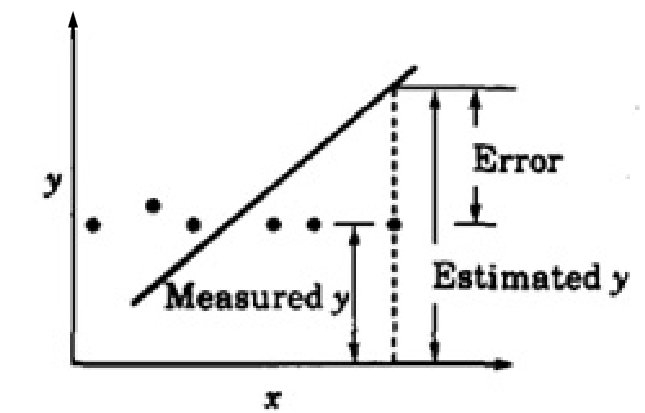
\includegraphics[width=0.5\textwidth]{figures/regression_error.png}
  \end{center}
  \caption{Definizione di residuo di regressione}\label{fig:residual-regression}
\end{figure}

\paragraph{Stima dei parametri di regressione}Come detto in precedenza, dato il modello in 
Equazione \ref{eq:simple_linear_regression_model}, si vogliono stimare i parametri di
regressione minimizzando la somma dei quadrati dell'errore e mantenendo l'errore medio a $0$.

\begin{equation}
  y_i = \beta_0 + \beta_1 x_i + \epsilon_i
  \label{eq:simple_linear_regression_model}
\end{equation}

Quindi si definisce la somma dei quadrati dell'errore come in Equazione
\ref{eq:squared_sum_error}, esplicitando $\epsilon_i$ dalla Equazione 
\ref{eq:simple_linear_regression_model}. 

\begin{equation}
  L = \displaystyle\sum_{i=1}^{n}\epsilon_i ^ 2 = \displaystyle\sum_{i=1}^{n} (y_i - 
  \beta_0 - \beta_1 x_i)^2
  \label{eq:squared_sum_error}
\end{equation}

Minimizzare la quantità al secondo membro della Equazione \ref{eq:squared_sum_error}
significa stimare $\beta_0$ e $\beta_1$ ponendo la derivata prima a zero. Quindi si procede
con il calcolo della derivata per entrambi i parametri in Equazione 
\ref{eq:lsq-error_derivative}\footnote{Si osserva che quello proposto è una stima per i 
parametri $\beta_0$ e $\beta_1$ in quanto essi dipendono dal singolo campione e pertanto 
sono funzioni di variabili aleatorie.}. 

\begin{align}
  \left\frac{\partial L}{\partial \beta_0}\right|_{\hat{\beta_0},\hat{\beta_1}} &= 
  -2 \displaystyle\sum_{i=1}^{n}(y_i - \hat{\beta}_0 - \hat{\beta}_1 x_i) = 0\\
  \left\frac{\partial L}{\partial \beta_1}\right|_{\hat{\beta_0},\hat{\beta_1}} &=
  -2 \displaystyle\sum_{i=1}^{n}(y_i - \hat{\beta}_0 - \hat{\beta}_1 x_i)x_i = 0
  \label{eq:lsq-error_derivative}
\end{align}

Applicando la proprietà di linearità, e semplificando il fattore $-2$ (data l'uguaglianza per 
$0$) si ottengono le \textbf{equazioni dei quadrati minimi normalizzate} in Equazione 
\ref{eq:lsq-normal-equation}.

\begin{align}
  \label{eq:lsq-normal-equation}
  n\hat{\beta}_0 + \hat{\beta}_1 \displaystyle\sum_{i=1}^{n} x_i &= 
  \displaystyle\sum_{i=1}^{n}y_i\\ 
  \hat{\beta}_0 \displaystyle\sum_{i=1}^{n}x_i + \hat{\beta}_1 \displaystyle\sum_{i=1}^{n}x_i^2 &= 
  \displaystyle\sum_{i=1}^{n}y_ix_i\\ 
\end{align}

Esplicitando dalla prima relazione in Equazione \ref{eq:lsq-normal-equation} $\beta_0$, si 
ottiene:
\[
  \hat{\beta}_0 = \frac{1}{n} \displaystyle\sum_{i=1}^{n}y_i - \frac{1}{n}
  \displaystyle\sum_{i=1}^{n}x_i = \overline{y} - \hat{\beta}_1\overline{x}
\]

Esplicitando dalla seconda relazione in Equazione \ref{eq:lsq-normal-equation} $\beta_1$, si 
ottiene:

\begin{align*}
  \hat{\beta_1} \displaystyle\sum_{i=1}^{n}x_i^2 &= \displaystyle\sum_{i=1}^{n}y_ix_i - 
  \hat{\beta_0} \displaystyle\sum_{i=1}^{n} x_i\\
  \hat{\beta_1} &= \displaystyle\frac{\displaystyle\sum_{i=1}^{n}y_ix_i - 
  \hat{\beta_0} \displaystyle\sum_{i=1}^{n} x_i} {\displaystyle\sum_{i=1}^{n}x_i^2}\\
  \hat{\beta_1} &= \displaystyle\frac{\displaystyle\sum_{i=1}^{n}(x_i - \overline{x})
  (y_i - \overline{y})}{\displaystyle\sum_{i=1}^{n}(x_i - \overline{x})^2}
\end{align*}

Quindi, i parametri di regressione stimati $\hat{\beta}_0$ e $\hat{\beta}_1$ sono:
\begin{enumerate}[label=(\alph*)] 
  \item $\hat{\beta_0} = \overline{y} - \beta_1\overline{x}$
  \item $\hat{\beta_1} = \displaystyle\frac{\displaystyle\sum_{i=1}^{n}(x_i - \overline{x})(y_i - \overline{y})}
    {\displaystyle\sum_{i=1}^{n}(x_i - \overline{x})^2}$
\end{enumerate}

\paragraph{Varianza dell'errore}Si dimostra che la somma dei quadrati dei residui ($SS_E$) 
costituisce un estimatore della varianza $\hat{\sigma}^2$ dell'errore $\epsilon$. Quindi 
definita la $SS_E$ come in Equazione \ref{eq:sse_definition}.
\begin{equation}
  SS_E = \displaystyle\sum_{i=1}^{n}e_i^2 = \displaystyle\sum_{i=1}^{n}(y_i - \hat{y}_i)^2
  \label{eq:sse_definition}
\end{equation}

Si può stimare la varianza dell'errore con:
\[
  \hat{\sigma}^2 = \frac{SS_E}{n-2}
\]
Siccome questo calcolo può risultare complicato, si può sostituire il modello 
$\hat{y} = \aht{\beta_0} + \hat{\beta_1}x_i$, ottenendo nuovamente l'espressione in Equazione
\ref{eq:squared_sum_error}. Passando alle varianze si ottiene:

\[
  SS_E = SS_T - \hat{\beta}_1 S_{xy}
\]

\subsubsection{Intervallo di confidenza per i parametri di regressioni}
È possibile stimare l'intervallo di confidenza per i parametri stimati $\hat{\beta_0}$ e 
$\hat{\beta_1}$. Se gli errori $\epsilon_i$ sono normalmente e indipendentemente distribuiti,
allora le distribuzioni:
\[
  \frac{\hat{\beta_1} - \beta_1}{\sqrt{\hat{\sigma}^2/S_{xx}}}
\]
e 

\[
  \frac{\hat{\beta_0} - \beta_0}
  {\sqrt{\hat{\sigma}^2[\frac{1}{n}+\frac{\overline{x}^2}{S_{xx}}]}}
\]
Seguono entrambe la distribuzione $t$ con $n-2$ gradi di libertà. Con queste due 
distribuzioni si può ottenere un intervallo a $100(1-\alpha)\%$ sia per il coefficiente 
angolare che per l'intercetto.

\paragraph{Intervallo di confidenza per il coefficiente angolare}Esplicitando $\beta_1$ 
dalla relazione precedente si ottiene l'intervallo di confidenza in Equazione
\ref{eq:ci-slope}.

\begin{equation}
  \hat{\beta_1}  - t_{\alpha/2,n-2} \sqrt{\hat{\sigma}^2/S_{xx}} \leq \beta_1 \leq 
  \hat{\beta_1}  + t_{\alpha/2,n-2} \sqrt{\hat{\sigma}^2/S_{xx}}
  \label{eq:ci-slope}
\end{equation}

\paragraph{Intervallo di confidenza per l'intercetto}Esplicitando $\beta_0$ 
dalla relazione precedente si ottiene l'intervallo di confidenza in Equazione
\ref{eq:ci-intercept}.

\begin{equation}
  \hat{\beta_0}  - t_{\alpha/2,n-2} \sqrt{\hat{\sigma}^2\left[\frac{1}{n}+
  \frac{\overline{x}^2}{S_{xx}}\right]} 
  \leq \beta_0 \leq 
  \hat{\beta_0}  + t_{\alpha/2,n-2} \sqrt{\hat{\sigma}^2\left[\frac{1}{n}+
  \frac{\overline{x}^2}{S_{xx}}\right]} 
  \label{eq:ci-intercept}
\end{equation}

\subsubsection{Analisi della varianza}
Dal punto di vista simbolico la $SS_T$ è la \textbf{\textit{total corrected sum of squares}}
e si esprime con:
\[
  SS_T = \displaystyle\sum_{i=1}^{n} (y_i - \overline{y})^2
\]

La $SS_R$ è la \textbf{\textit{regression sum of squares}} (differenza del valore predetto 
dalla media dei dati reali) e si esprime con:
\[
  SS_R = \displaystyle\sum_{i=1}^{n}(\hat{y}_i - \overline{y})^2
\]

Infine, si riporta la $SS_E$ \textbf{\textit{error sum of squares}}:

\[
  SS_E = \displaystyle\sum_{i=1}^{n} (y_i - \hat{y}_i)^2
\]

In Equazione \ref{eq:anova_identity}, si riporta la relazione di identità della varianza:

\begin{equation}
  SS_T = SS_R + SS_E \rightarrow \displaystyle\sum_{i=1}^{n}(y_i - \overline{y})^2 = 
  \displaystyle\sum_{i=1}^{n}(\hat{y}_i - \overline{y})^2 + 
  \displaystyle\sum_{i=1}^{n}(y_i - \hat{y}_i)^2
  \label{eq:anova_identity}
\end{equation}

Un fattore utile per capire la qualità di un modello di regressione è $R^2$ che misura 
la percentuale di varianza tenuta nel modello:
\[
  R^2 = \frac{SS_R}{SS_T} = \frac{SS_T - SS_E}{SS_T} = 1 - \frac{SS_E}{SS_T} 
\]
Questo indice però tende sempre ad aumentare al crescere della grandezza del campione. Per 
questo motivo è stato introdotta una versione corretta detta $R_{adj}^2$:
\[
  R_{adj}^2 = 1 - \frac{(1-R^2)(n-1)}{n-k-1}
\]
dove con $n$ si indica la grandezza del campione e con $k$ il numero di gradi di libertà.

\subsubsection{Assunzioni}
TODO MEGLIO
Il modello regressivo studiato si basa su alcune assunzioni che possono essere verificate con
test visivi:
\begin{itemize}
  \item Normalità dei residui con media nulla e deviazione standard costante
    (omoschedasticità): qq-plot dei residui + test statistici per verificare
    l'omoschedasticità;
  \item Linearità tra i predittori e la risposta;
  \item Errori indipendenti: scatter diagram dei residui per verificare l'assenza di trend;
\end{itemize}

\subsubsection{Test di regressione non parametrici: Mann-Kendall e stimatore di Theil-Sen}
Un test non parametrico non richiede la linearità e la normalità dei dati\footnote{Anche 
se non richiede la normalità dei dati, il \textit{Mann-Kendall} richiede che nel dataset 
non ci sia \textbf{autocorrelazione}.}. Il \textbf{\textit{Man Kendall}} è un test
statistico usato  per determinare l'esistenza di un trend positivo o negativo all'interno
di una serie di dati temporali e, in quanto tale, formula due ipotesi:

\begin{enumerate}[label=(\alph*)] 
  \item $H_0$: non c'è un trend monotonico;
  \item $H_1$: un trend monotonico è presente;
\end{enumerate}
Il test assume che l'ipotesi $H_0$ è vera e quindi i dati devono creare un dubbio ragionevole
tale da far rigettare $H_0$ e accettare $H_1$.

\paragraph{Coefficiente di correlazione di Mann-Kendall $\tau_A$}
In sintesi, il Mann-Kendall funziona calcolando $S$ definito come:
\[
  S = \sum_{i < j}sign(x_i - x_j)(y_i-y_j)
\]
$S$ è la definito come la somma delle coppie concordanti e discordanti(Figura 
\ref{fig:mannkendall}). Definito $S$, si può calcolare il coefficiente di correlazione
$\tau_A$ secondo l'Equazione \ref{eq:mannkendall-coeff}.

\begin{equation}
  \tau_A = \frac{S}{\binom{n}{2}} \to -1\leq \tau_A \leq 1
  \label{eq:mannkendall-coeff}
\end{equation}

\begin{figure}
  \begin{center}
    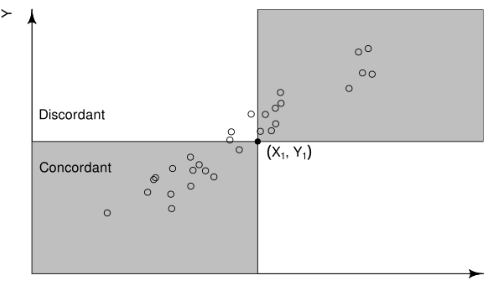
\includegraphics[width=0.6\textwidth]{./figures/regression_mannkendall.png}
  \end{center}
  \caption{Coefficiente $S$ per il test di Mann-Kendall}
  \label{fig:mannkendall}
\end{figure}

\paragraph{Stimatore di Theil-Sen}
Se un trend viene rilevato dal test di Mann-Kendall è possibile calcolare $\hat{\beta}_0$ e 
$\hat{\beta}_1$ attraverso il metodo di \textbf{\textit{Theil-Sen}} che prende la mediana
dei coefficienti angolari tra tutti i punti del dataset, calcolando $\forall (i,j)$

$$m = \frac{y_j - y_i}{x_j-x_i} $$
Un confronto tra il risultato il metodo dei quadrati minimi e lo stimatore di Sen è 
mostrato in Figura \ref{fig:lsq-vs-ths}.

\begin{figure}
  \begin{center}
    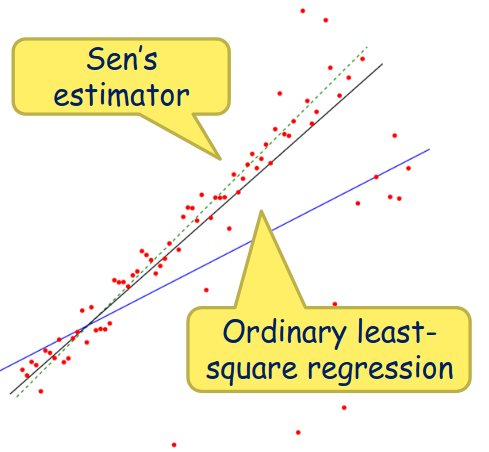
\includegraphics[width=.5\textwidth]{figures/regression_ths-vs-lsq.png}
  \end{center}
  \caption{Confronto tra metodo di Theil-Sen e quello dei quadrati minimi}
  \label{fig:lsq-vs-ths}
\end{figure}

\subsubsection{Regressione lineare multipla}
Al corso sono state introdotti anche altri modelli di regressione. Quello più vicino
a quello semplice e lineare studiato in precedenza è la regressione lineare con più
variabili predittrici, $x_1, x_2, \dots, x_k$ e una sola variabile di risposta $y$. 
Il modello quindi diventa:
\[
  y = b_0 + b_1x_1 + b_2x_2 + \dots + b_kx_k + e
\]
Che può essere scritto con la notazione matriciale in $y = Xb + e$ (Equazione 
\ref{eq:multiple-linear-regression-model}).In questo caso la $b$ può essere stimato
con:
\[
  b = (X^TX)^{-1}X^Ty
\]

\begin{equation}
  \begin{bmatrix}
    y_1 \\
    y_2 \\
    \vdots \\ 
    y_n 
  \end{bmatrix}
  = 
  \begin{bmatrix}
    1 & x_{11} & x_{12} & \cdots x_{1k} \\
    1 & x_{21} & x_{22} & \cdots x_{2k} \\
    . & . &  . & . \\ 
    1 & x_{n1} & x_{n2} & \cdots x_{nk}
  \end{bmatrix}
  \begin{bmatrix}
    b_0 \\
    b_1 \\
    \vdots \\ 
    b_k 
  \end{bmatrix}
  +
  \begin{bmatrix}
    e_1 \\
    e_2 \\
    \vdots \\ 
    e_n 
  \end{bmatrix}
  \label{eq:multiple-linear-regression-model}
\end{equation}
Anche in questo caso si può studiare la deviazione standard (Equazione 
\ref{eq:se-multiple-linear-regression}) dell'errore che a differenza del caso a
singolo predittore dipende da $k$.

\begin{equation}
  s_e = \sqrt{\frac{SS_E}{n-k-1}}
  \label{eq:se-multiple-linear-regression}
\end{equation}

\paragraph{Multi-collinearità}A differenza del caso a singolo predittore, quando ci 
sono $k$ variabili di regressione è possibile trarre dei risultati contradittori. 
Infatti, in un esperimento si può verificare che due fattori non risultano significanti
in quanto i loro intervalli di confidenza contengono lo zero, ma in realtà si nota che
essi sono dipendenti tra loro. La misura di dipendenza viene effettuata dalla misura 
di correlazione. Quindi questo significa che aggiungere variabili alla regressione non
sempre migliora i risultati, ma può addirittura rendere l'analisi meno precisa in 
quanto è molto probabile che i fattori aggiunti siano dipendenti tra loro. In questo 
caso è possibile risolvere il problema perdendo in precisione effettuando un'analisi 
a componenti principali \textit{PCA}, ma le componenti ottenute perdono di significato
fisico.

\paragraph{Variazione} Anche in questo caso è possibile determinare $R^2$ che resta 
una condizione necessaria ma non sufficiente per avere un buon modello. Inoltre,
sussiste la seguente realazione tra la somma dei quadrati e i gradi di libertà:
\[
  SS_T = SS_Y -  SS_0 = SS_R + SS_E \to n-1 = n - 1 = k + (n-k-1)
\]

con $SS_Y = \displaystyle\sum_{i=1}^{n}y_i^2$ e $SS_0 = n\overline{y}^2$.
\clearpage
\subsection{Analisi delle performance con modelli analitici}
I modelli analitici sono utili per studiare le performance di sistemi su cui non è
possibile effettuare misure dirette (magari ancora non esistono). Inoltre, da un
modello teorico è possibile estrarre valori nominali da confrontare con altre 
tecniche di analisi delle prestazioni

\subsubsection{Legge di Little}
Il modello più semplice a cui si può pensare per un sistema è quello di tipo\textbf{\textit{
  black-box}}(Figura \ref{fig:black-box}): una relazione ingresso-uscita. Nel caso ideale, si assume che il sistema abbia
memoria infinita: ogni richiesta viene accodata e sarà processata dopo un tempo $T$.
Sotto l'ipotesi di sistema ideale, detto $\lambda$ il tasso di arrivo delle richieste, si 
può affermare che il troughput corrisponde alle richieste in uscita a ritardate del tempo di 
risposta.

\begin{figure}
  \begin{center}
    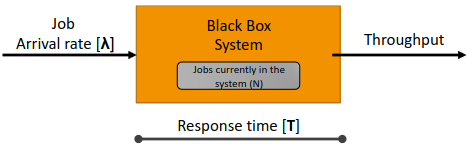
\includegraphics[width=.7\textwidth]{figures/mk-simple.png}
  \end{center}
  \caption{Modello black-box per un sistema}\label{fig:black-box}
\end{figure}

La legge di \textbf{Little} consente di stimare il numero medio di richieste all'interno di 
un sistema conoscendo il tempo medio di processamento $E[T]$ e il tasso di arrivo 
$\lambda$. In Equazione \ref{eq:little-law}, è mostrata l'espressione della legge di Little: 
si osserva che è applicabile solo ai valori medi. 
\begin{equation}
  E[N] = \lambda E[T]
  \label{eq:little-law}
\end{equation}

\paragraph{Esercizio}Si consideri un sistema di packet-inspection (Figura \ref{fig:little-ex})
in cui i pacchetti arrivano con $\lambda = 1/50ms$. Il firewall si compone di un primo filtro
che prevede un tempo di  attraverso $E[T_1] = 160ms$. Inoltre, se un pacchetto risulta
sospetto, bisogna attraversare un altro stadio di analisi con $E[T_2] = 400ms$. Si ipotizzi
che il $20\%$ dei pacchetti siano contrassegnati come sospetti, qual è il numero medio di
pacchetti nel sistema?

\begin{figure}
  \begin{center}
    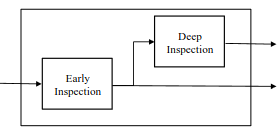
\includegraphics[width=.6\textwidth]{figures/mk-little-ex.png}
  \end{center}
  \caption{Sistema di packet inspectio nell'esercizio}\label{fig:little-ex}
\end{figure}

Il numero medio di pacchetti del sistema sarà dato dalla somma di quelli nei due componenti:
\[
  E[N] = E[N_1] + E[N_2]
\]

L'esercizio si risolve applicando la legge di little per entrambi i componenti del sistema. 
Nel primo stadio si ha che
\[
  E[N_1] = \lambda E[T_1] = \frac{1}{50}160 = 3.2
\]

Mentre, nel secondo ricordando :
\[
  E[N_2] = 0.2 \lambda E[T_2] = 0.2\frac{1}{50}400 = 1.6
\]

Quindi $E[N] = E[N_1] + E[N_2] = 3.2 + 1.6 = 4.8$

\subsubsection{Catene di Markov}
Il modello black-box con la legge di Little può essere utilizzato solo per fare analisi sui 
valori medi, per studiare sistemi più complicati bisogna usare modelli più complicati. 
Questa sezione introduce le \textbf{catene di Markov} che descrivono sistemi con stato in 
cui la transizione da uno stato all'altro dipende solamente dallo stato corrente. In sostanza
, le catene di Markov descrivono sistemi senza memoria.

\paragraph{Processo stocastico}Un processo stocastico è una famiglia vairabili aleatorie 
$\{X_t: t \in T\}$ dove $X_t$ è definita in $T \subseteq R_+ = [0, \infty)$. L'insieme di 
tutti i valori di $X_t\, \forall t \in T$ è detto spazio di stato e si indica con $S$. 
Se lo spazio di stato è formato da una quantità numerabile di elementi, il processo sarà
destto \textbf{discreto}, altrimenti sarà \textbf{continuo}. Si dice che il processo
stocastico è \textbf{indicizzato} dalla variabile $t$ (detta \textbf{parametro temporale}).

\paragraph{Processo di Markov}Un processo stocastico $\{X_t: t \in T\}$ costituisce un 
processo di Markov se per $t_0 < t_1 < \dots t_n$ lo  $X_{t_{n+1}}$ dipende solo da 
$X_{t_n}$ e non da $X_{t_0} < X_{t_1} \dots X_{t_{n-1}}$. Ovvero:
\begin{align}
  P(X_{t_{n+1}} &\leq s_{n+1} | X_{t_n} = s_n, X_{t_{n-1}} = s_{n-1}\dots X_{t_0} = s_0) \\
  &= P(X_{t_{n+1}} \leq s_{n+1}|X_{t_n} = s_n)
\end{align}

\paragraph{Sistemi omogenei} Un sistema si dice tempo-omogeno se la $CDF$ di $X_{t_{n+1}}$ 
non dipende dal periodo di osservazione me è invariante rispetto al tempo $t_n$: 
\[
  P(X_{t{n+1}} \leq s_{n+1} | X_{t_n} = s_n) = P(X_{t{n+1-t_n}} \leq s_{n+1} | X_{t_n} = s_n)
\]

\paragraph{DTMC - Catene di Markov a tempo discreto} Una catena di Markov a tempo discreto
è un processo stocastico discreto in cui risulta vera per ogni $n \in N_0$ la proprietà
Markov. Quindi dato $\{X_0, X_1, \dots X_n\}$ se vale che per $t_0 < t_1 < \dots t_n$
$X_{t_{n+1}}$ dipende solo da $X_{t_n}$ e non da $X_{t_0} < X_{t_1} \dots X_{t_{n-1}}$. 
Ovvero:
\begin{align}
  P(X_{t_{n+1}} &\leq s_{n+1} | X_{t_n} = s_n, X_{t_{n-1}} = s_{n-1}\dots X_{t_0} = s_0) \\
  &= P(X_{t_{n+1}} \leq s_{n+1}|X_{t_n} = s_n)
\end{align}

Quindi dato uno stato iniziale $s_0$, una DTMC evolve passo dopo passo nel suo stato 
secondo una matrice di transizione delle probabilità in cui $p_{ij}$ indica la probabilità
di passare nello stato $j$ stando nello stato $i$ ($i \to j$). Formalmente, indicando gli
stati con $i$ (corrisponde a $s_i$) e $j$ (corrisponde a $s_j$):
\begin{equation}
  p_{ij}(n) = P(X_{n+1} = j | X_n = i) = p_{ij} = P(X_1 = j | X_0 = i)\, \forall n \in T
  \label{eq:markov-matrix-prob}
\end{equation}

Nella Equazione \ref{eq:markov-matrix-prob}, si è assunto di essere in un sistema tempo 
invariante e, pertanto, è stata trascurata la $n$. La matrice delle transizioni sarà del 
tipo mostrata in Equazione \ref{eq:dtcm-matrix}. Le righe di questa matrice rappresentano
lo stato di partenza, mentre le colonne quello di destinazione raggiungibile in un solo passo.
In generale, si assume di essere in un grafo completamente connesso (tutti possono 
raggiungere tutti).
\begin{equation}
  P = \begin{bmatrix} 
    a_{11} & a_{12} & \dots \\
    \vdots & \ddots & \vdots \\
    a_{n1} & \dots & a_{nn} 
  \end{bmatrix}
  \label{eq:dtcm-matrix}
\end{equation}
Avendo una matrice delle transizioni, si può dedurre che si può rappresentare una catena di 
Markov come un grafo. Ad esempio in Figura \ref{fig:dtcm-ex}, è mostrato un semplice esempio 
di un grafo di una catena di Markov a tempo discreto a due stati, generato dalla generica
matrice:
\[
  P = \begin{bmatrix} 
    p_{00} & p_{01} \\
    p_{10} & p_{11} 
  \end{bmatrix}
\]

\begin{figure}
  \centering
  \begin{tikzpicture}[shorten >=2pt,node distance=6cm,on grid,auto]
    \tikzstyle{every state}=[fill={rgb:black,1;white,10},minimum size=2cm]

    \node[state] (s_0)                    {$s_0$};
    \node[state] (s_1)  [right of=s_0]    {$s_1$};

    \path[->]
    (s_0) edge [loop above] node {$p_{00}$}    (   )
    edge [bend left]  node {$p_{01}$}    (s_1)
    (s_1) edge [bend left]  node {$p_{10}$}    (s_0)
    edge [loop above] node {$p_{11}$}    (   )
  \end{tikzpicture}
  \caption{Esempio catena di Markov a tempo discreto per soli due stati}
  \label{fig:dtcm-ex}
\end{figure}

\paragraph{Evoluzione nello stato: transitorio e regime} La matrice in Equazione
\ref{eq:dtcm-matrix} spiega l'evoluzione del sistema in un singolo passo. È possibile
conoscere l'evoluzione del sistema dopo $n$ passi? Ad esempio, data la matrice $P$, si vuole
conoscere la probabilità che partendo dallo stato $i$, si arrivi allo stato $j$ dopo $2$
step. Formalmente, questo equivale a moltiplicare le probabilità che hanno come nodo di 
partenza $i$ e nodo destinazione $k$ ($k$ è qualsiasi nodo intermedio tra $i$ e $j$) e
quelle che hanno come nodo di destinazione $j$ partendo da $k$:
\begin{equation}
  P_{ij-2step} = \sum_k p_{ik}p_{kj}
  \label{eq:mk-2step}
\end{equation}

L'Equazione \ref{eq:mk-2step} viene dalla matrice $P^2$. Si può generalizzare questa
formula in:
\begin{equation}
  \pi(n) = \pi(n-1)P = \pi(n-2)P^2 = \dots = \pi(0)P^n
  \label{eq:state-evolution}
\end{equation}

L'Equazione \ref{eq:state-evolution} afferma che è possibile conoscere come evolverà lo stato 
del sistema in $n$ passi sapendo lo stato iniziale $\pi(0)$ e la matrice $P$.

Se esiste il limite
\[
  \lim_{n\to \infty}\pi(n) = \pi  
\]
allora $\pi$ è detto stato stabile e definisce la porzione di tempo in cui il sistema permane 
in ogni stato. Quando un sistema arriva in uno stato stabile non si hanno più informazioni 
sullo stato iniziale. Inoltre, quando ci si trova in uno stato stabile, bisogna soddisfare l'
equazione di equilibrio:
\begin{equation}
  \pi = \pi P \to \sum_i\pi_i = 1
  \label{eq:steady-state}
\end{equation}

\paragraph{Esercizio} Si consideri un sistema con $2$ processori che opera in slot di tempo:
in ogni slot può arrivare al più una richiesta. In ogni slot, può arrivare una richiesta con 
probabilità $\alpha = 0.5$. Quando un processore è occupato, può completare una richiesta con
probabilità $\beta = 0.7$. Il sistema opera scartando le richieste se quando questa arriva
entrambi i processori sono occupati, ma se uno finisce di lavorare ad una richiesta, quella
entrante viene accettata.
Calcolare:
\begin{itemize}
  \item L'efficienza del sistema;
  \item La frazione di richieste scartate;
\end{itemize}

Il sistema può essere modellato con una $DTCM$ a $3$ stati ed è rappresentata in Figura 
\ref{fig:dtcm-3state-ex}.

\begin{itemize}
  \item $0$: entrambi i processori sono liberi;
  \item $1$: un solo processore è occupato;
  \item $2$: entrambi i processori sono occupati;
\end{itemize}

Il fatto che possa arrivare una sola richiesta per slot vuol dire che non si può mai passare
dallo stato $0$ al $2$ (si assegna probabilità $0$ nella matrice $P$ al posto $(0,2)$)

\begin{figure}
  \centering
  \begin{tikzpicture}[shorten >=2pt,node distance=6cm,on grid,auto]
    \tikzstyle{every state}=[fill={rgb:black,1;white,10},minimum size=2cm]

    \node[state] (s_0)                    {$s_0$};
    \node[state] (s_1)  [right of=s_0]    {$s_1$};
    \node[state] (s_2)  [right of=s_1]    {$s_2$};

    \path[->]
    (s_0) edge [loop above] node {$p_{00}$}    (   )
    edge [bend left]  node {$p_{01}$}    (s_1)
    (s_1) edge [bend left]  node {$p_{10}$}    (s_0)
    edge [loop above] node {$p_{11}$}    (   )
    edge [bend left]  node {$p_{12}$}    (s_2)
    (s_2) edge [bend left]  node {$p_{20}$}    (s_0)
    edge [bend left]  node {$p_{21}$}    (s_1)
    edge [loop above] node {$p_{22}$}    (   )
  \end{tikzpicture}
  \caption{DTCM per l'esercizio con due processori}
  \label{fig:dtcm-3state-ex}
\end{figure}

La matrice che si genera dal sistema in Figura \ref{fig:dtcm-3state-ex} è:
\[
  P = \begin{bmatrix} 
    p_{00} & p_{01} & p_{02} \\
    p_{10} & p_{11} & p_{12} \\
    p_{20} & p_{21} & p_{22} 
  \end{bmatrix} = 
  \begin{bmatrix} 
    0.5 & 0.5 & 0 \\
    0.35 & 0.5 & 0.15 \\
    0.245 & 0.455 & 0.3
  \end{bmatrix}
\]

Le probabilità sono state semplicemente calcolate a partire da $\alpha$ e $\beta$ e i loro
valori complementari: sapendo che la probabilità che arrivi una richiesta è $\alpha = 0.5$, 
allora la probabilità che non arrivi sarà $\overline{\alpha} = 1 - \alpha = 1- 0.5 = 0.5$; 
mentre la probabilità che un processore non si liberi è $\overline{\beta} = 1 - \beta = 0.3$.
Inoltre, essendo le probabilità distribuite esponenzialmente, queste possono essere 
combinate: la probabilità che non arrivi una richiesta e che il sistema non termini quella
corrente è $1-\overline{\alpha}\overline{\beta}$. Ad esempio, la probabilità di effettuare
la transizione $s_2 \to s_0$ è quella che si liberino entrambi i processori e che non
arrivi nessuna richiesta ed equivale $p(2,0) = \overline{\alpha}\beta^2$.

Tornando alle domande dell'esercizio, l'efficienza $\epsilon$ è definita come segue:
\begin{itemize}
  \item $\epsilon=1$: tutti i processori sono occupati;
  \item $\epsilon=0.5$: un solo processore è occupato;
  \item $\epsilon=0$: i processori sono liberi;
\end{itemize}

Quindi l'efficienza totale è la probabilità di trovare un processore attivo sommata a quella
di avere entrambi i procssori attivi:
\[
  \epsilon = \frac{1}{2} \pi_1 + \pi_2
\]
Il numero di richieste perse è dato dalla probabilità di avere due processori occupati, 
nessuno dei due termina e arriva una nuova richiesta ed è esprimibile come:
\[
  P_{loss} = \alpha\overline{\beta}^2\pi_2
\]

Adesso, bisogna calcolare $\pi$, trovando il regime con l'Equazione \ref{eq:steady-state}. 
\[
  \pi = \pi P = \begin{bmatrix}
  \pi_0 & \pi_1 & \pi_2\end{bmatrix}
  = 
  \begin{bmatrix}
    \pi_0 & \pi_1 & \pi_2
  \end{bmatrix}
  \begin{bmatrix} 
    0.5 & 0.5 & 0 \\
    0.35 & 0.5 & 0.15 \\
    0.245 & 0.455 & 0.3
  \end{bmatrix}
\]
Da cui si ricava il sistema:

\begin{equation}
  \begin{cases}
    \pi_0 = 0.5\pi_0 + 0.35\pi_1 + 0.245\pi_2\\
    \pi_1= 0.5\pi_0 + 0.5\pi_1 + 0.455\pi_2\\
    \pi_2 = 0.15\pi_1 + 0.3\pi_2
  \end{cases} 
\end{equation}

Si dimostra che che il rango della matrice è sempre $n-1$. In questo caso, si hanno $2$ 
equazioni indipendenti, quindi si può sostituire una di queste con l'equazione di normalità. 
Si ottiene il sistema:

\begin{equation}
  \begin{cases}
    \pi_0 = 0.5\pi_0 + 0.35\pi_1 + 0.245\pi_2\\
    \pi_1= 0.5\pi_0 + 0.5\pi_1 + 0.455\pi_2\\
    \pi_0 + \pi_1 + \pi_2 = 1
  \end{cases} 
\end{equation}

Risolvendo numericamente si ottiene $\pi_0 = 0.399, \pi_1 = 0.494, \pi_2=0.107$.
Quindi l'efficienza è pari a $\epsilon = 0.494/2 + 0.107 = 0.354 \to \epsilon \approx 35\%$. 
Il numero di richieste perse dipende da $\pi_2$: $P_{loss} = (1-\beta)^2\alpha\pi_2 = 0.3^2 
\cdot0.5\cdot0.107 = 0.004815 \to P_{loss}\approx0.48\%$.


\paragraph{CTMC - Catene di Markov a tempo continuo}
Passando a un processo stocastico continuo una catena di Markov a tempo continua è analoga
a quella discreta tranne per il fatto che bisogna tenere in considerazione il tempo trascorso
uno stato. Il modello diventa leggermente differente in quanto  bisogna memorizzare
l'informazione in una nuova variabile (detta \textbf{\textit{holding time}}). In particolare,
la proprietà di Markov si riformula nel seguente modo: la probabilità di passare in uno stato
$s_j$ stando in $s_i$ non dipende da quanto tempo si spende in $s_i$ e in $s_k\, \forall k <
i$. L'unica distribuzione che può soddisfare la proprietà \textbf{\textit{memoryless}} è
l'esponenziale.

Dal punto di vista pratico, non è possible avere "autoanelli" in catene di Markov tempo 
contininuo poichè l'holding time (o tasso di transizione) specifica quante volte al secondo
uno stato deve essere attraversato. In questo caso si ha una matrice dei tassi di transizione 
$Q$:

\[
  q_{ij} = \begin{cases}
    h_ip_{ij}, &\text{ se }i\neq j\\
    -\sum_{i\neqj}q_{ij} = -h_i, &\text{ se } i = j
  \end{cases}
\]
$q_{ij}$ è la probabilità di rimanere nello stato $i$ o di andare in $j$. Per convenzione, 
sulla diagonale si posiziona il negato dell'holding time.

\paragraph{Evoluzione nello stato: transitorio e regime}
Valgono tutte le considerazioni fatte per le DTCM, quindi lo stato del sistema è fatta da 
un transitorio, che si esprime calcolando la derivata nel tempo:
\[
  \frac{d\,p(t)}{dt} = p(t)Q \to p(t) = c^{-Qt}
\]
Questo sistema ha infinite soluzioni, per sceglierne una si ha bisogno del vettore delle 
condizioni inziali $p(0)$.
,
La cosa interessante è il regime in cui la derivata $p(t) = 0$: analogamente al caso DTCM 
si definisce (se esiste) il limite:
\[
  \lim_{t\to\infty}p(t) = p
\]
Quindi le equazioni per la distribuzione stazionaria sono:
\begin{equation}
  \begin{cases}
    0 = pQ \\
    \sum_ip_i = 1
  \end{cases}
  \label{eq:ctcm-steady-state}
\end{equation}

\paragraph{Esercizio} Dato un sistema con due server $m_1$ e $m_2$. I tempi medi di 
servizio sono  distribuiti esponenzialmente con tassi $\mu_1 = 4/min$ e $\mu_2 = 2/min$. Il 
tasso di arrivo delle richieste è $\lambda = 5/min$. Se un task arriva e trova il primo 
server libero, allora lo occupa; se trova il secondo libero occupa il secondo, ma se sono 
entrambi occupati la richiesta viene scartata. Trovare:
\begin{itemize}
  \item Frazione di tempo in cui il server $2$ è utlizzato;
  \item Tempo medio di risposta di una richiesta;
\end{itemize}
L'esercizio risulta simile a quello nel caso DTCM, ma qui ci sono due server diversi e quindi
bisogna modellare la situazione con $2$ stati differenti: $m_1$ utilizzato, $m_2$ 
utilizzato. In Figura \ref{fig:ctcm-4state-ex}, è rappresentato il sistema modellato con 
$4$ stati.

\begin{figure}
  \centering
  \begin{tikzpicture}[shorten >=2pt,node distance=6cm,on grid,auto]
    \tikzstyle{every state}=[fill={rgb:black,1;white,10},minimum size=2cm]

    \node[state] (s_0)                    {$s_0$ idle };
    \node[state] (s_1)  [right of=s_0]    {$s_1,m_1$ busy};
    \node[state] (s_2)  [below of=s_1]    {$s_2,m_2$ busy};
    \node[state] (s_3)  [right of=s_1]    {$s_3$ both busy};

    \path[->]
    (s_0) edge [bend left]  node {$\lambda$}    (s_1)
    (s_1) edge [bend left]  node {$\lambda$}    (s_3)

    (s_1) edge [bend left]  node {$\mu_1$}    (s_0)

    (s_3) edge [bend left]  node {$\mu_2$}    (s_1)
    (s_3) edge [bend left]  node {$\mu_1$}    (s_2)

    (s_2) edge [bend left]  node {$\lambda$}    (s_3)
    (s_2) edge [bend left]  node {$\mu_2$}    (s_0)
  \end{tikzpicture}
  \caption{CTCM per l'esercizio con due processori}
  \label{fig:ctcm-4state-ex}
\end{figure}

Per capire l'utilizzazione di $m_2$, bisogna avere la probabilità di trovarsi in $s_2$ e 
$s_3$ a regime. Quindi $p_{m_2} = p_2 + p_3$. 

Invece il tempo medio di risposta si può trovare applicando la legge di Little (Equazione
\ref{eq:little-law}), ricavando il tempo di risposta medio come:
\[
  E[T] = \frac{E[N]}{\lambda_o}
\]
dove con $\lambda_o$ si è indicato il throughput del sistema.
Quindi, il numero medio di richieste nel sistema si calcola osservando che se il sistema è 
in $s_1$ o $s_2$ allora c'è una sola richiesta nel sistema. Altrimenti, ce ne sono $2$ in
$s_3$ e $0$ se si è in $s_0$
\[
  E[N] = 0\cdot p_0 + 1 \cdot (p_1 + p_2) + 2 \cdot p_3
\]
Mentre il throguhput $\lambda_o$ è dato dal tasso di uscita delle richieste in base allo 
stato in cui ci si trova. Ad esempio, in $s_3$ il tasso di uscita è $\mu_1 + \mu_2$. 
\[
  \lambda_o = 0\cdot p_0 + \mu_1 \cdot p_1 + \mu_2 \cdot p_2 + (\mu_1+\mu_2) \cdot p_3
\]
A questo punto, non resta che calcolare il vettore $p$ con l'equazione:
\[
  0 = pQ
\]
\paragraph{Processo Death-Birth}
Un processo Death-Birth è una catena di Markov tempo continuo (CTCM) semplificata in modo 
tale che le transizioni sono consentite solo tra gli stati adiacenti. Sono utili perchè 
consentono di utilizzare relazioni pre-confezionate che non richiedono la risoluzione di 
un sistema matriciale. In Figura \ref{fig:ctcm-death-bird}, un esempio di processo
Death-Bird. 

\begin{figure}
  \centering
  \begin{tikzpicture}[shorten >=2pt,node distance=6cm,on grid,auto]
    \tikzstyle{every state}=[fill={rgb:black,1;white,10},minimum size=2cm]

    \node[state] (s_i)                    {$s_{i-1}$};
    \node[state] (s_i+1)  [right of=s_0]    {$s_{i}$};

    \path[->]
    (s_i) edge [bend left]  node {$\lambda$}    (s_i+1)
    (s_i+1) edge [bend left]  node {$\mu$}    (s_i)
  \end{tikzpicture}
  \caption{Processo Death-Bird con $2$ stati}
  \label{fig:ctcm-death-bird}
\end{figure}

Infatti, tagliando una catena di Markov di tipo Death-Bird in un qualsiasi punto si 
definiscono $2$ stati: $s_i$ e $s_{i-1}$ (come in Figura \ref{fig:ctcm-death-bird}) 
caratterizzati da $\mu$ detto \textbf{tasso di morte} e $\lambda$ detto \textbf{tasso di 
nascita}. Per ogni coppia di stati del tipo $s_i$ e $s_{i-1}$ è possibile scrivere un'
equazione di \textbf{bilanciamento dettagliato} che assume il numero di richieste costanti:
\begin{equation}
  \mu_i p_i = \lambda_{i-1} p_{i-1}
  \label{eq:simple-deathbird-balance}
\end{equation}
Data la forma ricorsiva della relazione si può generalizzare per arrivare a dipendendere 
solo da $p_0$. Infatti, partendo dall'Equazione \ref{eq:simple-deathbird-balance}, si 
può esplicitare $p_{i}$ ed ottenere l'equazione di bilancio dettagliato generalizzata 
(Equazione \ref{eq:deathbird-balance}).

\begin{equation}
  \mu_i p_i = \lambda_{i-1} p_{i-1} \to p_i = \frac{\lambda_{i-1}}{\mu_i}p_{i-1} =
  \prod_{k=1}^n\frac{\lambda_{k-1}}{\mu_k}p_0
  \label{eq:deathbird-balance}
\end{equation}

Insieme all'Equazione \ref{eq:deathbird-balance}, si utilizza anche quella di
normalizzazione. Il processo Death-Birth può essere utilizzato anche per analizzare sistemi
con infiniti stati numerabili.
\[
  \sum_{i=1}^\infty p_i = 1
\]

\subsubsection{Teoria delle code}
La teoria delle code sfrutta i risultati delle catene di Markov per creare dei modelli usati
per analizzare le prestazioni di sistemi. Questi modelli sono contraddistinti da parametri
che si presentano nella loro configurazione generale come in Figura \ref{fig:queue-arch}.

\begin{itemize}
  \item Distribuzione dei tempi di arrivi dei processi $A(t)$;
  \item Distribuzione dei tempi di arrivi di partenza $D(t)$;
  \item Servizio $S_i(t)$;
  \item Capacità della coda $K_q$;
  \item Numero di server $n$;
  \item Disciplina di scheduling delle richieste $SD$;
\end{itemize}

\begin{figure}
  \begin{center}
    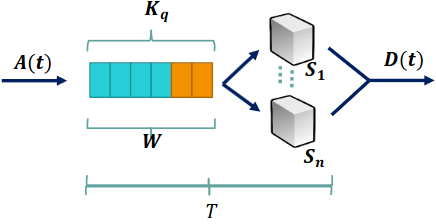
\includegraphics[width=.5\textwidth]{figures/queue-systems.png}
  \end{center}
  \caption{Rappresentazione grafica di un modello a coda}\label{fig:queue-arch}
\end{figure}

Solitamente come parametri prestazionali sono usati:
\begin{itemize}
  \item Tempo medio di attesa $W$;
  \item Tempo di risposta $T$;
  \item Throughput $\frac{D(t)}{t}$
\end{itemize}

Lo stato di questi modelli fa riferimento principalmente al numero di \textit{job} in una 
coda $N_q$, nei server $N_s$ e quello nel sistema $ N = N_q + N_s$.

\paragraph{Notazione di Kendall}Dato il grande numero di parametri per i modelli a coda, 
Kendall propose una notazione compatta nella forma \textbf{\textit{A/S/m/c/p/S.D.}} in cui:
\begin{itemize}
  \item con $A$ e $S$ si indica la distribuzione dei tempi di interarrivo e servizio. Con
    $M$ si indica un processo Markoviano, con $D$ deterministico, $G$ generico;
  \item $m$ è il numero di server presenti nel sistema;
  \item $c$ indica la grandezza della coda;
  \item $p$ dimensione della popolazione (numero di utenti che utilizza il sistema);
  \item $S.D$ disciplina di scheduling (default: First Come First Served);
\end{itemize}

Quando $p$ o $c$ sono omessi si assume un sistema con memoria e popolazione infinita. 
Ad esempio, in Figura \ref{fig:mm1-ex}, è mostrato un sistema a singola coda con tempi di
arrivo e di servizio markoviani con un un solo server. Il sistema ha capacità infinita.
Invece la Figura \ref{fig:mmm-ex}, mostra un sistema con $m$ server e tempi di arrivo e 
servizio markoviani. Infine, la Figura \ref{fig:mmmk-ex}, mostra un sistema con tempi di 
arrivo e servizio markoviani, composto da $m$ server con un buffer di dimensione $K$.

\begin{figure}
  \centering
  \begin{subfigure}{0.3\textwidth}
    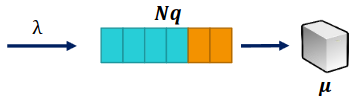
\includegraphics[width=.95\textwidth]{figures/queue-mm1.png}
    \caption{Sistema M/M/1}
    \label{fig:mm1-ex}
  \end{subfigure}\hfil
  \begin{subfigure}{0.3\textwidth}
    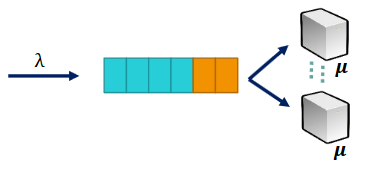
\includegraphics[width=.95\textwidth]{figures/queue-mmm.png}
    \caption{Sistema M/M/m}
    \label{fig:mmm-ex}
  \end{subfigure}\hfil
  \begin{subfigure}{0.3\textwidth}
    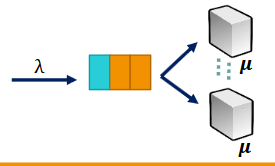
\includegraphics[width=.95\textwidth]{figures/queue-mmmk.png}
    \caption{Sistema M/M/m/K}
    \label{fig:mmmk-ex}
  \end{subfigure}
  \caption{Esempi di sistemi modellati con la teoria delle code}
\end{figure}

\paragraph{Processo di Poisson}Nel corso si studiano per la maggior parte sistemi senza 
memoria (tempi di arrivo e servizio markoviani). Come già detto, l'unica distribuzione che 
rispetta la proprietà di Markov è quella esponenziale con tasso $\lambda$. Se il tempo di 
arrivo per i processi nel sistema è distribuito in maniera esponenziale con tasso costante,
allora il processo viene detto di \textbf{Poisson} e ha la seguente distribuzione:
\[
  P_n(t) = \frac{(\lambda t)^n}{n!} e^{-\lambda t}
\]
Il processo di Poisson è importante perchè permette di sfruttare la proprietà \textbf{PASTA}
che consente di affermare che:
\begin{equation}
  E[W] = E[N]\cdot E[S]
  \label{eq:pasta-property}
\end{equation}
il tempo medio di attesa in una coda è dato dal numero medio di utenti nel sistema per il
tempo di servizio.

\paragraph{Modelli a singola coda $M/M/1$} Si parte con lo studio di un sistema a singola 
coda, $m=1$ e un \textit{buffer} infinito. Questo tipo di sistema viene modellato con 
un processo nascita-morte in cui gli stati sono ordinati a seconda del numero di utenti 
nel sistema. Quindi lo stato $0$ a cui è associata $p_0$ avrà zero utenti, mentre quello 
$n+1$ avrà $n$ utenti.

Si ricorda che la distribuzione stazionaria è:
\[
  \lambda p_{n-1} = \mu p_n \to p_n = \frac{\lambda}{\mu}p_{n-1}
\]
da cui si ricava il fattore di utilizzo $\rho = \frac{\lambda}{\mu}$. Ripetendo i passaggi 
per esprimere la distribuzione stazionaria in funzione di $p_0$ si ottiene che:
\[
  p_n = \rho^n p_0
\]
Osservando che $\rho < 1$, applicando la proprietà di normalizzazione all'equazione di 
bilancio del processo nascita-morte, si ottiene che:
\[
  \sum_{i=1}^\infty p_i = 1 \implies p_0\sum_{i=1}^\infty\rho^i = 1 \implies p_0 = 1 -\rho
\]
Quindi si può riscrivere l'equazione di $p_n$ come:
\[
  p_n = \rho^n(1-\rho)
\]
Gli indicatori di performance sono in Tabella \ref{tab:mm1-perf}. 

\begin{table}
  \begin{center}
    \begin{tabular}[c]{l|l}
      \hline
      \multicolumn{1}{c|}{\textbf{Metrica}} & 
      \multicolumn{1}{c}{\textbf{Espressione}} \\
      \hline
      Utilizzazione & $\rho$ \\
      Numero medio di utenti & $ E[N] = \frac{\rho}{1-\rho}$ \\
      Tempo di risposta medio & $E[T] = \frac{1}{\mu - \lambda}$\\
      Tempo di attesa medio & $E[W] = E[T] -  \frac{1}{\mu} = \frac{\rho}{\mu-\lambda}$\\
      Utenti in coda & $E[N_Q] =\lambda E[W] = \frac{\rho^2}{1-\rho}$\\
      \hline

    \end{tabular}
  \end{center}
  \caption{Indicatori di performance principali per un sistema M/M/1}
  \label{tab:mm1-perf}
\end{table}

Il numero medio degli utenti del sistema $E[N]$ è calcolato a partire dalla definizione di 
media:
\[
  E[N]=\sum_{i=0}^\infty ip_i = (1-\rho)\sum_{i=0}^\infty i\rho^i 
\]
Portando fuori un $\rho$ dall sommatoria si può applicare la proprità della derivata:
\[
  E[N]=\rho(1-\rho) \sum_{i=0}^\infty i\rho^{i-1} = \rho(1-\rho)\frac{d}{d\rho}
  \left(\frac{1}{1-\rho}\right)
  = \frac{\rho}{1-\rho}
\]
Il tempo di risposta medio è dato dalla legge di Little:
\[
  E[T] = \frac{E[N]}{\lambda}= \frac{\rho}{\lambda(1-\rho)} = \frac{\lambda/\mu}
  {\lambda(1-\lambda/\mu)}
  = \frac{1/\mu}{1-\lambda/\mu} = \frac{1}{\mu - \lambda} 
\]

Il tempo di attesa si ricava sottraendo da quello totale $E[T]$ quello di servizio:
\[
  E[W] = E[T] - E[S] = \frac{1}{\mu -\lambda} - \frac{1}{\mu} = \frac{\mu - \mu + \lambda}
  {\mu(\mu-\lambda)} = \frac{\lambda}{\mu(\mu-\lambda)} = \frac{\rho}{\mu-\lambda}
\]
Infine, anche per il numero di utenti in coda si applica la legge di Little:
\[
  E[N_Q] = \lambda E[W] = \frac{\rho^2}{1-\rho}
\]

\paragraph{Esercizio: dimensionamento di una coda} Su un server HTTP single-thread arrivano
richieste che vengono servite in sequenza. $\lambda=8500/min$ e $1/\mu = 4ms$. Entrambe le
distribuzioni sono esponenziali. Quale è la minima lunghezza delle coda $L$ tale che una
richiesta non trova la coda piena con una probabilità del $99.99\%$?

Si usa un modello $M/M/1$. Detti $L$ utenti in coda, l'esercizio chiede di calcolare la
probabilità di avere $L+2$ utenti nel sistema (uno in arrivo, un in esecuzione e $L$ in coda). 
In un modello $M/M/1$, $P(N > L +2) = 1 - P(N < L + 2)$. Per come è create la catena di 
Markov, bisogna calcolare:
\[
  1 - P(N < L + 2) = 1 - \sum_{i=0}^{L+1}p_i = 1 - (1-\rho)\sum_{i=0}^{L+1} \rho^i
\]
Dato che $\rho < 1$, si può scrivere:
\[
  P(N > L + 2) = 1 - (1-\rho) \frac{1 - \rho^{L+1+1}}{1-\rho} = 1 - 1 + \rho^{L+2} = \rho^{L+2}
\]

Imponedo questa quantità minore di $1 - 0.9999\%$, si ha che:
\[
  \rho^{L+2} < (1-0.9999)^4 < -4 = (L+2)\log(\rho) \implies L > 14.2175
\]

\paragraph{Modelli con $m$ server $M/M/m$} Analogamente al caso precedente, si mostra in Figura 
\ref{fig:ctcm-mmm} la catena di Markov. Rispetto al caso a singola coda il tasso di morte, 
aumenta fino a raggiungere lo stato $m$ (numero di server del sistema). A partire dallo 
stato $m$, il tasso di morte diventa $m\mu$. Dopo lo stato $m$, il sistemd diventa analogo 
ad un $M/M/1$ più veloce.

\begin{figure}
  \begin{center}
    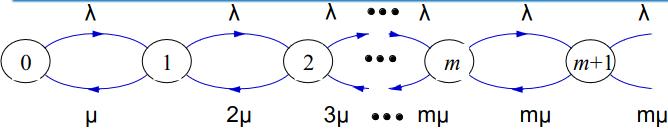
\includegraphics[width=.75\textwidth]{figures/queue-mmm-ctmc.png}
  \end{center}
  \caption{Catena di Markov associata al modello $M/M/m$}\label{fig:ctcm-mmm}
\end{figure}

In questo caso, bisogna modellare il throughput a seconda se $i>m$ o $i\leq m$.
\begin{cases}
  \lambda p_{i-1} = i\mu p_i, &\text{ se } i < m\\
  \lambda p_{i-1} = m \mu p_i, &\text{ se } i \geq m\\
\end{cases}

Qui si definiscono $2$ parametri:
\begin{itemize}
  \item $\alpha = \frac{\lambda}{\mu}$: intensità di traffico;
  \item $\rho = \frac{\alpha}{m} = \frac{\lambda}{m\mu}$: intensità di traffico per server;
\end{itemize}
Omettendo le dimostrazioni:
\[
  p_0 = \frac{1-\rho}{1+\rho}
\]
Inoltre, grazie alla proprietà PASTA:
\[
  P_q = \sum_{i=0}^\infty p_i = 2p_0 \sum_{i=0}^\infty \rho^i = \frac{2p_0}{1-\rho}
\]
In Tabella \ref{tab:mmm-perf}, sono riassunti i nuovi indicatori di performance.

\begin{table}
  \begin{center}
    \begin{tabular}[c]{l|l}
      \hline
      \multicolumn{1}{c|}{\textbf{Metrica}} & 
      \multicolumn{1}{c}{\textbf{Espressione}} \\
      \hline
      Utenti in coda & $E[N_Q] =\lambda E[W] =  \frac{2\rho^3}{1-\rho^2}$\\[2ex]
      Numero medio di utenti & $ E[N] = \frac{2\rho}{1-\rho^2}$ \\[2ex]
      Tempo di attesa medio & $E[W] = P_q \frac{1}{2\mu-\lambda}$\\[2ex]
      Tempo di risposta medio & $E[T] = \frac{1}{\mu}+ P_q\frac{1}{2\mu - \lambda}$\\[2ex]
      \hline
    \end{tabular}
  \end{center}
  \caption{Indicatori di performance principali per un sistema M/M/m con buffer infinito}
  \label{tab:mmm-perf}
\end{table}

\paragraph{Modello a singola coda $m$ server e capacità $K$} Questo modello rappresenta il 
caso in cui la dimensione della coda sia $K$. Quando una richiesta arriva e la coda è piena,
allora questa viene scartata. Il modello $M/M/m/K$ è una catena di Markov a $K+1$ stati,
mostrata in Figura \ref{fig:mmmk-ctmc}, l'Equazione di normalizzazione diventa:
\[
  \sum_{i=0}^Kp_i = 1
\]

\begin{figure}
  \begin{center}
    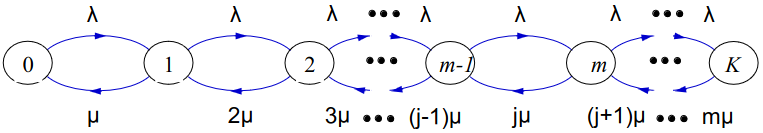
\includegraphics[width=0.95\textwidth]{figures/queue-mmmk-ctmc.png}
  \end{center}
  \caption{Catena di Markov per il modello $M/M/m/K$}\label{fig:mmmk-ctmc}
\end{figure}

In questo tipo di sistema, si è interessati a conoscere quando la coda si riempie $P(N=K)=p_k$. 
Questo valore rappresenta la frazione di tempo che il sistema spende in uno stato di blocco e,
pertanto viene detto \textbf{\textit{Time blocking}}.

Un altro aspetto fondamentale dei sistemi con memoria finita è il tasso di richieste scartate
$\lambda p_k$. $p_k$ può essere usato per calcolare il throughput $\lambda(1 - p_k)$(ottenuto 
attraverso la legge di Little)

\paragraph{Sistemi con perdita} Una particolare classe di sistemi modellati con $M/M/m/K$ 
sono quelli in cui $K=m$. In pratica, questi sistemi non hanno una coda: se tutti i server
sono impegnati le richieste vengono perse. Detto $\alpha = \frac{\lambda}{\mu}$, la 
probabilità di perdita è: 
\[
  P_B(m, \alpha) = p_m = \frac{1}{m!} \frac{\alpha^m}{\sum_{i=0}^m \frac{\alpha^i}{i!}}
\]
Questa formula mette in relazione la grandezza del sistema, l'intesità del traffico $\alpha$ 
e la Quality of Service.

\paragraph{Modelli a singola coda con popolazione finita $p$}Questo tipo di modelli viene 
utilizzato quando si conosce la popolazione di utenti: ogni utente può effettuare richieste
con un certo tasso $\lambda$ e tra una richiesta e l'altra vi è il cosidetto
\textbf{\textit{Thinking time}} (Figura \ref{fig:user-behaviour}). Quando un utente effetua
una richiesta, deve aspettare di avere una risposta per poterne sottomettere un'altra.

\begin{figure}
  \centering
  \begin{tikzpicture}[shorten >=2pt,node distance=6cm,on grid,auto]
    \tikzstyle{every state}=[fill={rgb:black,1;white,10},minimum size=2cm]

    \node[state] (0)                    {Thinking state};
    \node[state] (1)  [right of=s_0]    {Service state};

    \path[->]
    (0) edge [bend left]  node {$\lambda$}    (1)
    (1) edge [bend left]  node {$\mu$}    (0)
  \end{tikzpicture}
  \caption{Diagramma di comportamento degli utenti}
  \label{fig:user-behaviour}
\end{figure}

I modelli con popolazione finita sono stabili in quanto la catena di Markov sottostante ha 
una dimensione finita. Infatti, è anche inutile specificare $K > N$, in quanto il sistema 
non può avere più di $N$ richieste nel sistema. 

La catena di Markov utilizzata per un sistema $M/M/m/K/N$ è mostrata in Figura
\ref{fig:mmmkp-ctmc}. Allo stato $0$ possono arrivare $N\lambda$ richieste ($0$ utenti hanno
sottomesso la loro richiesta), nello stato $1$ possono arrivare ancora $(N-1) \lambda$ 
richieste ($1$ utente ha inviato la richiesta), così via fino a $(N-m)\lambda$ in cui si 
satura il throughput $m\mu$ e infine a $(N-K+1)\lambda$ in cui il sistema scarta le 
richieste.

\begin{figure}
  \begin{center}
    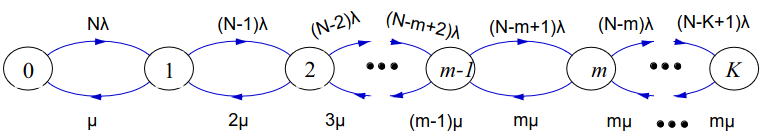
\includegraphics[width=0.95\textwidth]{figures/queue-mmmkp-ctmc.png}
  \end{center}
  \caption{Catena di Markov per un sistema $M/M/m/K/p$}\label{fig:mmmkp-ctmc}
\end{figure}

Purtroppo però, i processi di arrivo non sono Poissoniani: ogni volta che un utente fa la
richiesta modifica il tasso di arrivo dei lavori. Quindi non vale la proprietà PASTA, anche
se i processi restano Markoviani.

Per studiare questi sistemi, si fa uso della proprietà dell'osservatore: la probabilità di 
stare nello stato $j$ con $N$ utenti quando arriva una richiesta è pari alla probabilità di 
stare nello stato $j$ con $N-1$ utenti in un momento qualsiasi.

\paragraph{Esempio: web-server} Si consideri un gruppo di $N$ web client ciascuno con 
think time esponenziale con $\lambda = 15s$ che fanno richieste a un singolo server con tempo
di servizio esponenziale con $\mu = 1s$. Il sistema risultante è un modello $M/M/1/N/N$.
Come varia il tempo di risposta in base la numero di utenti $N$?

Il sistema può essere modellato con la catena di Markov in Figura \ref{fig:mmmnn-ctmc}.

\begin{figure}
  \begin{center}
    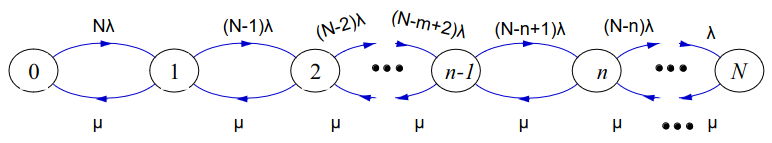
\includegraphics[width=0.95\textwidth]{figures/queue-mmmkp-webserver.png}
  \end{center}
  \caption{Catena di Markov per il web server $M/M/m/N/N$}\label{fig:mmmnn-ctmc}
\end{figure}
La probabile a regime che ci siano $n$ richieste nel sistema è:
\[
  p_n = \frac{N!}{(N-n)!}\rho^n \cdot p_0
\]
Dove la probabilità che il server sia in idle è:
\[
  p_0 = \left(\sum_{i=0}^N\frac{N!}{(N-n)!}\rho^n\right)^{-1}
\]

Il throughput si calcola moltiplicando $\mu$ per la probabilità di trovarsi in tutti gli 
stati tranne lo $0$:
\[
  E[R] = \mu(1 - p_0)
\]
Un client fa una richiesta sommando il tempo di risposta e il \textbf{thinking time}:
\[
  E[T] + \frac{1}{\lambda}
\]
Il tasso di richieste totale sul client è:
\[
  \frac{N}{E[T] + \frac{1}{\lambda}}
\]
In uno stato stabile, il throughput sui client è uguale a quelli dal sistema:
\[
  \frac{N}{E[T] + \frac{1}{\lambda}} = \mu(1 -p_0)
\]

\paragraph{Modelli con tempi di servizio non esponenziali}Si vuole studiare come evolve un
sistema i cui tempi di sistema sono non markoviani. In particolare, si vuole esaminare un
sistema $M/G/1$ (arrivi poissoniani, tempi di servizio generici). Quindi il numero di utenti
nel sistema non è un processo di Markov: il throughput dipende da quanto tempo ha speso
l'utente nel sistema.

Il tempo di attesa medio è dato dal numero di utenti in coda per la media del tempo di 
servizio a cui si aggiunge il lavoro rimanente da effettuare nel server:
\begin{equation}
  E[W] = E[N_q] E[S] + E[R]
  \label{eq:waiting-mg}
\end{equation}
Applicando la legge di Little, $E[N_q] = \lambda E[W] \implies E[W] = \frac{E[R]}{1 -\rho}$ 

I sistemi con tempi di servizio generici possono essere studiati con la formula di 
\textbf{\textit{Pollaczek-Khinchin}} (detta PK). Questa formula si basa sull'osservare che il 
tempo medio di lavoro rimanente da fare su un server si comporta come un triangolo: è 
massimo quandoa arriva una richiesta su un certo tempo e poi scende linearmente. In Figura 
\ref{fig:pk}, è riportato un grafico in cui si rappresenta questo fenomeno. 

\begin{figure}
  \begin{center}
    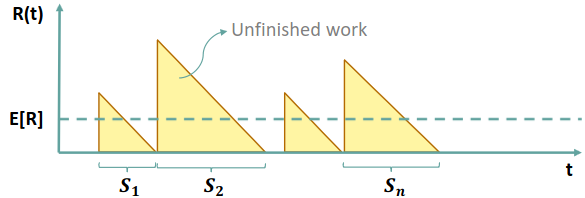
\includegraphics[width=.7\textwidth]{figures/queue-pk.png}
  \end{center}
  \caption{Tempo di lavoro rimanente secondo Pollaczek-Khincin}\label{fig:pk}
\end{figure}
Assumento l'arrivo poissoniano, in $(0,T)$ arrivano $n$ richieste che corrispondo a $n$ 
triangoli. Secondo PK, $E[R]$ può essere stimato come la media delle aree dei triangoli su $t$:
\[
  E[R] = \frac{1}{t}\sum_{i=1}^n \frac{1}{2}S_i^2 \implies 
  E[R] = \frac{n}{t} \frac{1}{n}\sum_{i=1}^n \frac{1}{2}S_i^2
\]

Ricordando che $n=\lambda t$, la relazione diventa:
\[
  E[R] = \frac{\lambda}{2}\frac{1}{n}\sum_{i=1}^n S_i^2 = \frac{\lambda}{2}E[S^2]
\]

Quindi la PK può essere usata per calcolare $E[W]$, sostituendola in Equazione 
\ref{eq:waiting-mg} con $E[N_q] = \lambda E[W]$.

\begin{align*}
  E[W] &= E[N_q]E[T] + E[R] \\ 
  &= \lambda E[W]E[T] + \frac{\lambda}{2}E[S^2]\\
  E[W] (1-\lambda E[T]) &= \frac{\lambda}{2}E[S^2]\\
  E[W] &= \frac{\lambda E[S^2]}{2(1-\rho)}
\end{align*}

In Tabella \ref{tab:mg-perf}, sono riassunti gli altri indicatori di performance.
\begin{table}
  \begin{center}
    \begin{tabular}[c]{l|l}
      \hline
      \multicolumn{1}{c|}{\textbf{Metrica}} & 
      \multicolumn{1}{c}{\textbf{Espressione}} \\
      \hline
      Utenti in coda & $E[N_Q] =\lambda E[W] = \frac{\lambda^2 E[S^2]}{2(1-\rho)}$\\[2ex]
      Numero medio di utenti & $ E[N] = \lambda E[T] = \lambda E[S] + \frac{\lambda^2 E[S^2]}
      {2(1-\rho)}$ \\[2ex]
      Tempo di attesa medio & $E[W] = \frac{\lambda E[S^2]}{2(1-\rho)}$\\[2ex]
      Tempo di risposta medio & $E[T] = E[S] +E[W] = E[S]+\frac{\lambda E[S^2]}{2(1-\rho)}$\\[2ex]
      \hline
    \end{tabular}
  \end{center}
  \caption{Indicatori di performance principali per un sistema M/G/m con buffer infinito}
  \label{tab:mg-perf}
\end{table}

\paragraph{Reti di code}Per reti di code si intende lo studio dell'interconnessione di 
diversi sistemi a singola coda riutilizzando quanto già visto e concentrandosi sulla
particolare topologia. Quindi, si considera un sistema composto da $n$ sottosistemi: lo stato
sarà costituito dal numero di utenti nel sistema e può essere rappresentato come una tupla in 
cui l'$i$-esimo elemento rappresenta il numero di task per ogni sottosistema.

La topologia di un sistema con code può essere definito in maniera probabilistica, non tutti
gli utenti sono dello stesso tipo e alcune richieste possono usare un insieme di risorse 
(anch'esso definito in maniera probabilistica), insomma: ci sono molte variabili in gioco. 

La prima distinzione che si può fare sulle topologie è quella di \textbf{\textit{closed 
network}} (Figura \ref{fig:closed-network}) e \textbf{\textit{open network}} (Figura
\ref{fig:open-network}). La prima non ha input dall'esterno, la sua popolazione è definita
da $K$ utenti ed è molto utile per modellare processi su calcolatori. Al contrario, le open
network prevedono una popolazione non costante in quanti le richieste arrivano dall'esterno
e richiedono risorse con una certa probabilità. Queste topologie sono specificate da una 
matrice di routing in cui ogni elemento indica la probabilità di andare in un sottosistema
$j$ stando in $i$.

\begin{figure}
  \centering
  \begin{subfigure}{0.5\textwidth}
    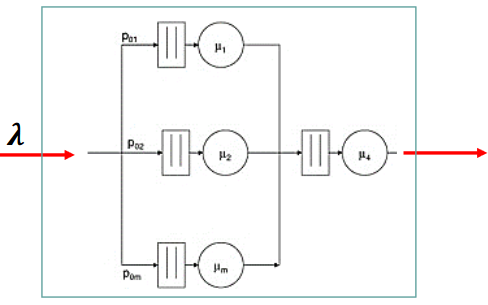
\includegraphics[width=.95\textwidth]{figures/queue-open-network.png}
    \caption{Esempio: open network}
    \label{fig:open-network}
  \end{subfigure}\hfil
  \begin{subfigure}{0.5\textwidth}
    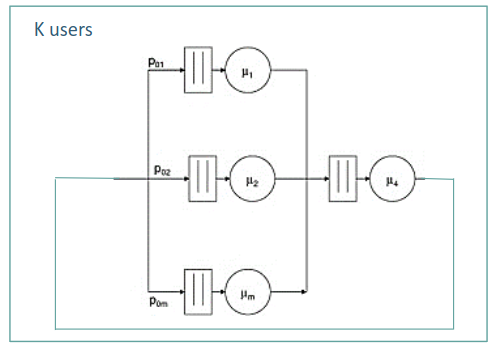
\includegraphics[width=.828\textwidth]{figures/queue-closed-network.png}
    \caption{Esempio: closed network}
    \label{fig:closed-network}
  \end{subfigure}
  \caption{\ref{fig:open-network} Rete aperta: le richieste arrivano con un tasso $\lambda$. 
  \ref{fig:closed-network} Rete chiusa: le richieste provengono da una popolazione $K$ interna}
\end{figure}

\paragraph{Product form networks}Queste reti sono molto semplici in quanto possono essere 
viste come una serie di $M/M/1$ in cascata. In Figura \ref{fig:product-form}, un esempio di
\textit{product form network}. Si tratta di reti aperte in cui l'uscita di un componente è
l'ingresso della coda del successivo. Sarebbe impensabile creare una catena di Markov 
poichè ci sarebbero troppi stati.

Sotto le assunzioni di:
\begin{itemize}
  \item tempi di arrivo esponenziali;
  \item componenti con memoria infinita;
  \item disciplina di scheduling FCFS;
  \item solo su reti aperte senza loop;
  \item topologia indipendente dallo stato;
\end{itemize}

\begin{figure}
  \begin{center}
    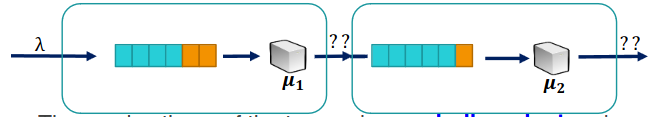
\includegraphics[width=0.95\textwidth]{figures/queue-product-form-network.png}
  \end{center}
  \caption{Esempio: rete di tipo product form}\label{fig:product-form}
\end{figure}

si possono studiare con il \textbf{teorema di Burke} che afferma: in una topologia aperta 
con code di tipo $M/M/m$ senza loop schedulate con FCFS è possibile analizzare i sistemi di 
code in maniera indipendente:
\[
  P(N =\{n_1, n_2\}) = P(N_1 = n_1)\cdot P(N_2 = n_2) \implies p(n_1)p(n_2) = 
  \rho_1^{n_1}(1-\rho_1)\rho_2^{n_2}(1-\rho_2)
\]
ovvero è una forma per dire che l'uscita di una coda $M/M/m$ è ancora un processo di Poisson.
Per questo motivo sono dette reti product form: malgrado il numero enorme di assunzioni sono
semplici da analizzare perchè si moltiplicano i prodotti. In Tabella 
\ref{tab:product-form-perf}, sono riassunte le metriche di perfomance.

\begin{table}
  \begin{center}
    \begin{tabular}[c]{l|l}
      \hline
      \multicolumn{1}{c|}{\textbf{Metrica}} & 
      \multicolumn{1}{c}{\textbf{Espressione}} \\
      \hline
      Numero medio di utenti & $E[N] = E[N_1] + E[N_2] $\\[2ex]
      Tempo di risposta medio & $E[T] = E[T_1] +E[T_2]$\\[2ex]
      \hline
    \end{tabular}
  \end{center}
  \caption{Indicatori di performance per una di rete Product Form con le ipotesi di Burke}
  \label{tab:product-form-perf}
\end{table}

\paragraph{Rete di Jackson}Una rete di Jackson è sempre una rete aperta, ma con meno ipotesi
rispetto a quella product form: ci possono essere loop. La presenza di loop fa cadere le 
ipotesi di Burke in quanto lo stato del sistema dipende dallo stato delle code che può
essere influnzato da altri componenti. In Figura \ref{fig:jackson}, è mostrato un esempio di 
rete di Jackson.

\begin{figure}
  \begin{center}
    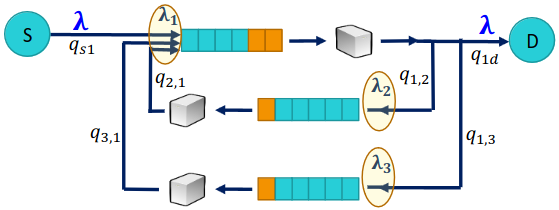
\includegraphics[width=0.65\textwidth]{figures/queue-jackson-network.png}
  \end{center}
  \caption{Esempio: rete di Jackson}\label{fig:jackson}
\end{figure}

Data una matrice di routing $Q$, le equazioni principali di una rete di Jackson sono quelle
di \textbf{conservazione del flusso}: in ogni nodo $i$ il flusso di ingresso $\lambda_i$ è 
pari alla somma dei flussi delle altre stazioni pesate per la probabilità di arrivare in $i$ 
a cui si somma anche la probabilità di arrivare in $i$ direttamente dall'ingresso $\lambda$. 
\[
  \lambda_i = \lambda q_{s,i} + \sum_{j=1}^K \lambda_jq_{j,i}
\]
Inoltre, poichè si sta immaginando di avere code a memoria infinita, nessuna richiesta viene
scartata:
\[
  \lambda = \sum_{j=1}^K \lambda_jq_{j,d}
\]
Dove con $q_{j,d}$ si è indicato tutti i nodi che conducono all'uscita del sistema $d$.

Infine, il seguente teorema afferma che nelle reti di Jackson, anche se non ci sono arrivi 
poissoniani nelle stazioni, lo stato di queste stazioni si comporta come se lo fossero. 
Quindi vale ancora la proprietà per la quale la probabilità che la rete si trovi in un
certo stato, è pari alla produttoria delle probabilità dei singoli sistemi. 
\[
  p(n) = \prod_{i=0}^Kp_i(n_i)
\]
Con questo teorema, ipotizzando di avere tutte code $M/M/1$, si ottiene la Tabella 
\ref{tab:jackson-perf}.

\begin{table}
  \begin{center}
    \begin{tabular}[c]{l|l}
      \hline
      \multicolumn{1}{c|}{\textbf{Metrica}} & 
      \multicolumn{1}{c}{\textbf{Espressione}} \\
      \hline
      Numero medio di utenti per nodo & $E[N_i] = \frac{\rho_i}{1-\rho_i} $\\[2ex]
      Tempo di risposta medio per nodo& $E[T_i] = \frac{E[N_i]}{\lambda_i} = \frac{1}{\mu_i-\lambda_i}$\\[2ex]
      Tempo di risposta totale medio & $E[T] = \frac{E[N]}{\lambda} = \frac{1}{\lambda}\sum_{i=1}^K \frac{\rho_i}{1-\rho_i}$\\[2ex]

      \hline
    \end{tabular}
  \end{center}
  \caption{Indicatori di performance per una rete di Jackson con code $M/M/1$}
  \label{tab:jackson-perf}
\end{table}

\paragraph{Esempio: rete di Jackson} Si consideri un sistema in cui i task possono richiedere
l'I/O durante un operazione. In particolare, durante un'esecuzione un task può richiedere
un'operazione di I/O con probabilità $q$ oppure uscire con probabilità $1-q$. Trovare il 
tempo di risposta medio per un task. 

\begin{figure}
  \begin{center}
    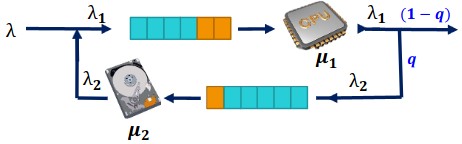
\includegraphics[width=.6\textwidth]{figures/queue-jackson-ex-network.png}
  \end{center}
  \caption{Modello esercizio rete di Jackson}\label{fig:ex-jackson}
\end{figure}

In Figura \ref{fig:ex-jackson}, è rappresentato lo schema per l'esercizo proposto. Bisogna
usare la formula:
\begin{equation}
  E[T] = \frac{1}{\lambda} \sum_{i=1}^K \frac{\rho_i}{1-\rho_i}
  \label{eq:jackson-ex}
\end{equation}
In questo caso, $\lambda_1 = \lambda + \lambda_2$, mentre $\lambda_2 = q\lambda_1 $. 
$\lambda_1$ e $\lambda_2$ si trovano risolvendo il sistema:
\begin{equation}
  \begin{cases}
    \lambda_1 = \lambda + \lambda_2 \\
    \lambda_2 =  q \lambda_1   
  \end{cases}
  \label{eq:}
\end{equation}
Da cui si ottiene che $\lambda_1 = \frac{\lambda}{1-q}$, mentre $\lambda_2 = 
\frac{\lambda q}{1-q}$

Dalla legge di Little: $E[T] = \frac{E[N]}{\lambda}$. Dall'Equazione \ref{eq:jackson-ex}, si 
ottiene che $E[N] = \frac{\rho}{1-\rho}$, quindi:
\[
  E[T] = \frac{1}{\lambda}\left(\frac{\rho_1}{1-\rho_2}+\frac{\rho_2}{1-\rho_2}\right)
\]

\paragraph{Reti chiuse}Una rete chiusa ha il vantaggio di avere un numero di stati finiti
poichè ha una popolazione finita di $K$. Purtroppo, gli arrivi non sono poissoniani e quindi
non si può applicare la proprietà PASTA. Gli stati di una rete con $M$ stazioni e $K$ utenti
sono:
\[
  \binom{M-K-1}{M-1}  
\]

Un esempio di rete chiusa è mostrato in Figura 
\ref{fig:gn-network}. Questa si può studiare sempre con l'equazione di conservazione del 
flusso che in questo caso risulta ancora più semplice poichè non ci sono nodi sorgente e 
destinazione. 
\[
  \lambda_i = \sum_{j=0}^K \lambda_j q_{j,i}
\]

\begin{figure}
  \begin{center}
    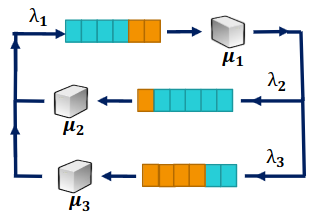
\includegraphics[width=0.5\textwidth]{figures/queue-gn-network.png}
  \end{center}
  \caption{Rete chiusa di esempio}\label{fig:gn-network}
\end{figure}

L'equazione di conservazione del flusso non può essere risolta poichè genera $n-1$ equazioni
indipendenti. In genere si esprime il vettore $\lambda$ in funzione di un parametro
$\alpha$ e $\hat{\lambda}_i$. Quest'ultimo fattore prende il nome di \textbf{flow ratios} e 
indica la percentuale di utenti che arriva al componente $i$; $\alpha$ dipende dal totale 
di utenti nel sistema.

Il teorema di \textbf{Gordon-Newell} afferma che reti chiuse possono essere viste come quelle
product form: la probabilità di trovarsi in uno stato è esprimbile come prodotto a meno 
di un fattore di normalizzazione. Inoltre, questo prodotto non dipende da $\alpha$. 

\begin{equation}
  p(n) = \begin{cases}
    \frac{1}{G} \prod_{i=0}^K \hat{\rho}_i^{n_i}, &\text{ se } \sum_i n_i = K\\
    0, &\text{ se } \sum_i n_i \neq K
  \end{cases}
  \label{eq:gordon-newell}
\end{equation}

Il fattore di normalizzazione $G$ presentato in Equazione \ref{eq:gordon-newell}, è:
\[
  G = \sum_{n: \sum_in_i = K}\prod_{i=i}^K \rho_i^{n_i}
\]

\paragraph{MVA - Mean Value Analysis}
In una rete con processi non poissoniani, non si può applicare la proprietà PASTA. Quindi,
si utilizza la tecnica del Mean Value Analysis basata sulla proprietà dell'osservatore. 
La proprietà deriva dallo studio di un sistema con $0$ utenti e ragionando su cosa può
succedere quando arriva il primo job. Generalizzando il ragionamento si ottiene che il 
tempo di risposta del nodo $i$ è dato dal tempo di servizio per tutti gli utenti in coda a 
cui si aggiunge il tempo di servizio per la richiesta corrente:
\[
  T_i[K] = \frac{1}{\mu_i} + N^*_i[K]\frac{1}{\mu_i}
\]
Dove con $N^*_i$ si esprima la proprietà dell'osservatore, ottenendo la formula:
\[
  T_i[K] = \frac{1}{\mu_i} + N_i[K-1]\frac{1}{\mu_i} = (1+N_i[K-1]) \frac{1}{\mu_i}
\]
Per trovare il numero medio di utenti nel sistema si procede nel seguente modo:
\begin{align*}
  N_i[K] = K\frac{N_i[K]}{K} = K \frac{N_i[K]}{\sum_{j=1}^M N_j[K]}
\end{align*}
Applicando la legge di Little $N = \lambda T$, si ottiene:
\[
  N_i[K] = K \frac{\lambda_i[K]T_i[K]}{\sum_{j=1}^M \lambda_j[K]T_j[K]}
\]
Assumendo che  $\lambda_i[K] = \alpha\hat{\lambda_i}$:
\[
  N_i[K] = K \frac{\hat{\lambda}_iT_i[K]}{\sum_{j=1}^M \hat{\lambda_j}T_j[K]}
\]
Quindi sempre applicando la legge di Little, si ottiene il tasso di arrivo delle richieste:
\[
  \lambda_i = \frac{N_i[K]}{T_i[K]} = K \frac{\hat{\lambda}_i}{\sum_{j=1}^M \hat{\lambda_j}T_j[K]}
\]
\clearpage
\section{DoE - Design of experiment}
Le prestazioni di un sistema spesso si dipendendono da uno o più fattori. L'analisi di 
performance dovrebbe cercare di isolare gli effetti dei singoli fattori e cercare di capire
quale è effettivamente significativo. Nel design of experiment vale la seguente tassonomia:
\begin{itemize}
  \item \textbf{Risposta}: variabile osservata in un esperimento;
  \item \textbf{Fattori}: variabili che influenzano la risposta, sono anche detti predittori
    o variabili predittive;
  \item \textbf{Livelli}: i fattori possono assumere un numero di valori finito;
  \item \textbf{Fattori primari}: fattori di cui si è in grado di quantificare gli effetti 
    sulla risposta;
  \item \textbf{Fattori secondari}: fattori di cui non si è in grado (o non si è interessati) 
    di quantificare glieffetti sulla risposta;
  \item \textbf{Replicazioni}: un insieme di esperimenti può essere ripetuto per un numero 
    $r$ di volte;
  \item \textbf{Design sperimentale}: un design sperimentale consiste nello specificare il 
    numero di esperimenti. Per ciascuno dei quali bisogna specificare la combinazione del 
    livello dei fattorie il numero di replicazioni;
  \item \textbf{Interazioni}: due fattori possono avere un effetto combinato sulla variabile
    di risposta. Ad esempio, dati due fattori $A$ e $B$ con soli due blivelli $A_1$, $A_2$, 
    $B_1$ e $B_2$, può succedere che $y$ aumenta se $A_1 \to A_2$ in maniera indipendente 
    da $B$ (in questo caso non c'è interazione tra il $A$ e $B$). Se invece $y$ varia in 
    maniera differente a seconda del valore assunto da $B$ allora i due fattori interagiscono.
\end{itemize}

Gli obiettivi di un design sperimentale sono:
\begin{itemize}
  \item Studiare gli effetti dei fattori controllabili sulla risposta capendo quali sono i 
    più fluente;
  \item Studiare l'interazione tra i fattori;
  \item Sviluppare un modello per descrivere i dati;
  \item Caratterizzare gli errori di misura;
\end{itemize}

\subsection{Simple design}
Il \textbf{\textit{simple design}} consiste nel partire con una configurazione semplice e 
far variare uno per volta i fattori per ognuno dei livelli per vedere come viene influenzata
la risposta. Dati $k$ fattori, ognuno dei quali può assumere $n_i$ livelli, il numero di 
esperimenti $n$ è mostrato in Equazione \ref{eq:simple-design}.
\begin{equation}
  n = 1 + \displaystyle\sum_{i=1}^{k}(n_i - 1)
  \label{eq:simple-design}
\end{equation}

Questo tipo di esperimento risulta vantaggioso in quanto il numero di esperimenti cresce 
linearmente con il numero di fattori, ma risulta poco utile in quanto non vengono testate 
tutte le combinazioni di livelli di fattori e pertanto è possibile che gli effetti di 
interazione sia o trascurati.


\subsection{Full factorial design}
Il \textbf{\textit{Full factorial design}} offre una copertura esaustiva di tutte le 
combinazioni dei livelli. Pertanto, con $k$ fattori di cui l'$i$-esimo $n_i$ livelli, risulta
:
\[
  n = \prod_{i=1}^kn_i
\]
Spesso, è impossibile fare un numero di esperimento così elevato e per questo motivo si 
ricorre a design frazionali. In particolare, si cerca di ridurre il numero di livelli che un
fattore può assumere.

\subsubsection{$2^k$ factorial design}
Il tipo di factorial design più utilizzato è $2^k$: $k$ fattori che assumono solo $2$ livelli
(di solito corrispondono al valore minimo e al valore massimo) ottenendo $n = 2^k$.

\paragraph{Esempio: $2^2$ factorial design}
L'esperimento più semplice che si può pensare di mettere in piedi è quello con $k = 2$. 
Avendo in mente gli obiettivo del \textit{DoE}, si effettua una regressione non lineare
(Equazione \ref{eq:2factorial-design-model}) per isolare il contributo dei fattori e la loro
interazione per la variabile di risposta. Per avere dei valori numerici, si fa riferimento 
ai dati mostrati in Tabella \ref{tab:experimental-design}.

\begin{table}
  \begin{center}
    \begin{tabular}[c]{|c|c|c|}
      \hline
      \multicolumn{1}{|c|}{\textbf{$x_A$}} & 
      \multicolumn{1}{c|}{\textbf{$x_A$ - Minimo}} & 
      \multicolumn{1}{c|}{\textbf{$x_B$ - Massimo}} \\

      \hline
      Minimo & 15 & 45 \\
      Massimo & 25 & 75\\

      \hline
    \end{tabular}
    \caption{Dati sperimentali con design $2^2$}\label{tab:experimental-design}
  \end{center}
\end{table}

Avendo solo due livelli, è convenzione assegnare 
il valore $-1$ quando il fattore assume il livello minimo e $1$ quello massimo (Equazione 
\ref{eq:2factorial-design-xa} e Equazione \ref{eq:2factorial-design-xb}).

\begin{equation}
  y = q_0 + q_A x_A + q_B x_B + q_{AB} x_Ax_B
  \label{eq:2factorial-design-model}
\end{equation}

\begin{equation}
  x_A = 
  \begin{cases}
    -1, &\text{ $x_a$ è minimo }\\
    +1, &\text{ $x_a$ è massimo }
  \end{cases}
  \label{eq:2factorial-design-xa}
\end{equation}

\begin{equation}
  x_B = 
  \begin{cases}
    -1, &\text{ $x_b$ è minimo }\\
    +1, &\text{ $x_b$ è massimo }
  \end{cases}
  \label{eq:2factorial-design-xb}
\end{equation}

In Eqauzione \ref{eq:2factorial-design-model}, $q_0$ è dovuto alle performance medie, 
$q_A$ e $q_B$ rappresentano gli effetti dei singoli fattori e $q_{AB}$ esprime l'interazione 
dei due fattori. Esistono due modi per trovare questi parametri:
\begin{enumerate}
  \item Si risolve il sistema presentato in Equazione \ref{eq:2factorial-design-parameters};
  \item Si usa il metodo della \textbf{\textit{sign table}};
\end{enumerate}

\begin{equation}
  \begin{cases}
    y_1 = q_0 + q_A + q_B + q_{AB}, &\text{ con }x_A = +1, x_B = +1 \\
    y_2 = q_0 + q_A - q_B - q_{AB}, &\text{ con }x_A = +1, x_B = -1\\
    y_3 = q_0 - q_A + q_B - q_{AB}, &\text{ con }x_A = -1, x_B = +1\\
    y_4 = q_0 - q_A - q_B + q_{AB}, &\text{ con }x_A = -1, x_B = -1\\
  \end{cases}
  \label{eq:2factorial-design-parameters}
\end{equation}

Sostituendo i dati dalla Tabella \ref{tab:experimental-design}, si ottiene il sistema in 
Equazione \ref{eq:2factorial-design-parameter-calc} che risolto restituisce i 
$q_0 = 40$, $q_A = 20$, $q_B= 10$, $q_{AB} = 5$.

\begin{equation}
  \begin{cases}
    75 = q_0 + q_A + q_B + q_{AB}, &\text{ con }x_A = +1, x_B = +1 \\
    25 = q_0 + q_A - q_B - q_{AB}, &\text{ con }x_A = +1, x_B = -1\\
    45 = q_0 - q_A + q_B - q_{AB}, &\text{ con }x_A = -1, x_B = +1\\
    15 = q_0 - q_A - q_B + q_{AB}, &\text{ con }x_A = -1, x_B = -1\\
  \end{cases}
  \label{eq:2factorial-design-parameter-calc}
\end{equation}

Tuttavia il metodo più utilizzato è quello della tabella dei segni. Si costruisce una 
tabella $2^kx2^k$ con le seguenti colonne:
\begin{enumerate}
  \item $I$: colonna per $q_0$ riempita con tutti $1$;
  \item $A$: colonna per $q_A$ riempita con tutti i possibili valori di $x_A$;
  \item $B$: colonna per $q_B$ riempita con tutti i possibili valori di $x_B$;
  \item $AB$: colonna per $q_B$ riempita con i prodotti su riga delle colonne $A$ e $B$;
  \item $y$: colonna in cui si riporta la variabile di uscita;
\end{enumerate}

In Tabella \ref{tab:ex-sign-method}, è mostrato l'esempio relativo ai dati iniziali.

\begin{table}[h]
  \begin{center}
    \begin{tabular}[c]{|c|c|c|c|c|}
      \hline
      \multicolumn{1}{|c|}{\textbf{$I$}} & 
      \multicolumn{1}{c|}{\textbf{$A$}} & 
      \multicolumn{1}{c|}{\textbf{$B$}} & 
      \multicolumn{1}{c|}{\textbf{$AB$}} & 
      \multicolumn{1}{c|}{\textbf{$Y$}} \\ 

      \hline
      1 & 1 & 1 & 1 & 75 \\
      1 & -1 & 1 & -1 & 25 \\
      1 & 1 & -1 & 1 & 45 \\
      1 & -1 & -1 & 1 & 15 \\
      \hline
    \end{tabular}
    \caption{Esempio metodo \textit{sign table}}
    \label{tab:ex-sign-method}
  \end{center}
\end{table}

Si procede nel seguente modo:
\begin{itemize}
  \item Per ottenere $q_0$ si moltiplicano gli elementi della colonna $I$ con quelli della 
    colonna $y$, la somma viene divisa per $2^k$. Quindi nell'esempio $q_0 = \frac{75\cdot1 + 
    25\cdot1 + 45\cdot1 + 15\cdot1}{4} = \frac{160}{4} = 40$
  \item Per ottenere $q_A$ si moltiplicano gli elementi della colonna $A$ con quelli della 
    colonna $y$, la somma viene divisa per $2^k$. Quindi nell'esempio $q_A = \frac{75\cdot1 - 
    25\cdot1 + 45\cdot1 - 15\cdot1}{4} = \frac{80}{4} = 20$
  \item Per ottenere $q_B$ si moltiplicano gli elementi della colonna $B$ con quelli della 
    colonna $y$, la somma viene divisa per $2^k$. Quindi nell'esempio $q_B = \frac{75\cdot1 + 
    25\cdot1 - 45\cdot1 - 15\cdot1}{4} = \frac{40}{4} = 10$
  \item Per ottenere $q_{AB}$ si moltiplicano gli elementi della colonna $AB$ con quelli della 
    colonna $y$, la somma viene divisa per $2^k$. Quindi nell'esempio $q_{AB} = \frac{75\cdot1
    - 25\cdot1 - 45\cdot1 + 15\cdot1}{4} = \frac{20}{4} = 5$
\end{itemize}

\paragraph{Allocazione delle variazione: importanza} L'\textbf{importanza}\footnote{
  L'importanza non è un concetto statistico in quanto misura di un rapporto. La significatività
  esprime la percentuale di varianza rispetto all'errore e necessita di un'analisi a parte.} 
di un fattore si misura come la percentuale di 
variazione che questo esprime sulla totale. Quindi data la $SS_T = 
\sum_{i=1}^n(y_i - \overline{y})^2 = 2^2q_A^2 + 2^2q_B^2 + 2^2q_{AB}^2$
Quindi si ritorna all'equazione di allocazione della variazione:
\[
  SS_T = SS_A + SS_B + SS_{AB}
\]

Ad esempio l'importanza del fattore $A$ può essere calcolata come 
\[
  V_A = \frac{SS_A}{SS_T}
\]
\subsubsection{$2^{k}r$ factorial design}
Questo tipo di esperimento prevede l'utilizzo di $r$ ripetizioni. In questo modo è possibile
dare una stima dell'errore sperimentale. Ragionevolmente questo si definisce come:
\[
  e_{ij} = y_{i} - \hat{y}_i
\]

Un eperimento con $r$ ripetizioni non ha una sola varaibile di risposta, ma un vettore di 
$y_{ij}$ di cui si calcola ,la media $\hat{y}_i$. Quindi il modello presentato in Equazione
\ref{eq:2factorial-design-model} prende una componente legata all'errore che si aggiunge a 
$q_0$ e diventa:
\begin{equation}
  y = q_0 + q_A x_A + q_B x_B + q_{AB}x_Ax_B + e
  \label{eq:2kr-factorial-design-model}
\end{equation}

Quindi, in base all'Equazione \ref{eq:2kr-factorial-design-model}, si ricava una relazione
in cui si esprime la variazione dei dati trovando:
\begin{equation}
  SS_T = SS_A + SS_B + SS_{AB} + SS_E = 2^krq_A^2 + 2^krq_B^2 + 2^krq_{AB}^2 + SS_E
  \label{eq:2kr-variation}
\end{equation}

Dove $SS_E$ è la somma dei quadrati dell'errore che, riprendendo la definizione precedente 
risulta:
$$SS_E = \sum_{i=1}^{2^k}\sum_{j=1}^r e_{ij}^2$$

\paragraph{Esempio: $3\cdot2^2$ factorial design}
Analogmante al caso $2^2$ factorial design, in Tabella $\ref{tab:ex-2kr-sign-method}$ è 
riportata l'applicazione del metodo dei segni per il calcolo degli effetti e dell'errore.

\begin{table}[h]
  \begin{center}
    \begin{tabular}[c]{|c|c|c|c|c|c|}
      \hline
      \multicolumn{1}{|c|}{\textbf{$I$}} & 
      \multicolumn{1}{c|}{\textbf{$A$}} & 
      \multicolumn{1}{c|}{\textbf{$B$}} & 
      \multicolumn{1}{c|}{\textbf{$AB$}} & 
      \multicolumn{1}{c|}{\textbf{$y$}} & 
      \multicolumn{1}{c|}{\textbf{$\hat{y}$}} \\ 

      \hline
      1 & -1 & -1 & 1 & $(15,18,12)$ &15 \\
      1 & 1 & -1 & 1 & $(45,48,51)$ & 48 \\
      1 & -1 & 1 & -1 & $(25,28,19)$& 24 \\
      1 & -1 & -1 & 1 & $(75,75,81)$ & 77 \\
      \hline
    \end{tabular}
    \caption{\textit{Sign table} per esempio $2^kr$}
    \label{tab:ex-2kr-sign-method}
  \end{center}
\end{table}

Risolvendo il modello si ottiene che $q_0 = 41$, $q_A = 21.5$, $q_B = 9.5$, $q_{AB} = 5$.

In Tabella \ref{tab:ex-2kr-error-estimate}, sono stati trovati i residui $e_{ij}$ che saranno
utilizzati per il calcolo di $SS_E$.

\begin{table}[h]
  \begin{center}
    \begin{tabular}[c]{|c|c|c|c|c|c|c|}
      \hline
      \multicolumn{1}{|c|}{\textbf{$\hat{y}_i$}} & 
      \multicolumn{1}{c|}{\textbf{$y_{i1}$}} & 
      \multicolumn{1}{c|}{\textbf{$y_{i2}$}} & 
      \multicolumn{1}{c|}{\textbf{$y_{i3}$}} & 
      \multicolumn{1}{c|}{\textbf{$e_{i1}$}} & 
      \multicolumn{1}{c|}{\textbf{$e_{i2}$}} & 
      \multicolumn{1}{c|}{\textbf{$e_{i3}$}} & 

      \hline
      15 & 15 & 18 & 12 & 0 & 0 & -3 \\
      48 & 45 & 48 & 51 & -3 & 0 & 3 \\
      24 & 25 & 28 & 19 & 1 & 4 & 5 \\
      77 & 75 & 75 & 81 & -2 & -2 & 4 \\
      \hline
    \end{tabular}
    \caption{Calcolo degli errori in $2^kr$}
    \label{tab:ex-2kr-error-estimate}
  \end{center}
\end{table}

Quindi, si può calcolare la somma dei quadrati utilizzando la relazione in Equazione
\ref{eq:2kr-variation}:
\begin{itemize}
  \item $SS_A = 12 \cdot (21.5)^2 = 5547$;
  \item $SS_B = 12 \cdot (9.5)^2 = 1083$;
  \item $SS_{AB} = 9 + 9 + 9 + 9 +1 +16+ 25 +4+ 4 +16 = 102$;
\end{itemize}

Quindi $SS_T = 5547 + 1083 + 102 = 7032$. Ad esempio vale:
\[
  V_A = \frac{5547}{7032} = 78.88\%
\]
Mentre l'errore esprime lo $1.45\%$ della variazione.

\subsection{Fractional design}
Il design frazionale è utile perchè riduce di molto il numero di esperimenti da fare 
contendo budget e costi di un'analisi. Il costo da pagare per quest semplificazione è
quello di commettere un errore rispetto al numero di fattori in quanto ne vengono considerati
una quantità minore.
\subsubsection{$2^{k-p}$ fractional factorial design}
In questo tipo di design, $p$ indica il numero di fattori trascurati: avendo $n = 2^{k-p}$, 
si osserva che che per $p=1$ si dimezzano gli esperimenti e per $k=2$ si riducono di un 
quarto. 

La preparazione di una \textit{sign table} per un $2^{k-p}$ design è analoga a quella
classica ma le colonne devono avere un significato particolare. In particolare, bisogna:
\begin{itemize}
  \item Disegnare la \textit{sign table} con un $k-p$ fattori come visto nel full factorial
    design;
  \item Aggiungere la colonna $I$ relativa alle prestazioni medie a quelle già disegnate;
  \item Marcare le $k-p$ con i $k-p$ scelti per effetuare gli esperimenti;
  \item Tutte le altre colonne sono i prodotti dei $k-p$ fattori indicati in precedenza;
  \item Tra le $2^{k-p}-k+p-1$ colonne a destra e marcarle con i $p$ fattori che non 
    sono stati scelti nel passo precedente;
\end{itemize}

\paragraph{Confounding effect}
Come si intuisce facilmente, partendo da $k$ fattori, la \textit{sign table} dovrebbe avere
una dimensione $2^kx2^k$. Quindi effettuando $2^{k-p}$ esperimenti si avrà una tabella più
piccola e alcuni effetti risultano trascurati. 

Precisamente, in un design $2^{k-p}$, $2^p$ effetti sono confusi insieme. La confusione che
si ottiene in un design è una scelta. 

La disciplina che si occupa di rispondere a questa domanda è l'algebra della confusione che
si basa su due semplici regole:
\begin{enumerate}
  \item La media $I$ è l'unità: $IA = A$;
  \item Ogni termine elevato al quadrato si elimina: $A^2BCD = BCD$;
\end{enumerate}

Per generare tutti gli effetti confusi si utilizza il \textbf{polinomio generatore} che
corrisponde a quello che esprime la media $I$. Per ottenerlo basta moltiplicare qualsiasi 
effetto confuso con la parte ad sinistra dell'equazione. Ad esempio, dato l'effetto confuso
$D = AB$, moltiplicando a destra per $D$ si ottiene $D^2 = ABD \to I = ABD$. Dato il 
polinomio generatore è possibile avere gli altri effetti confusi moltiplicando entrambi i 
membri per il fattore desiderato. Ad esempio, dato il polinomio generatore $I = ABD$, per 
ottenere la parte confuso con $A$, si ottiene $I = ABD \to A = A^2BD $, ricordando che i 
quadrati si ignorano, si ottiene $A = BD$.

Cosa distingue un buon design da un altro? Si parla di \textbf{risoluzione del design} 
(\textbf{\textit{design resolution}}) e si intende il minimo ordine degli effetti che si
stanno confondendo. In un $2^{k-p}$ design, la risoluzione è il minimo ordine degli effetti
confusi con la $I$. In generale, si preferiscono design ad alta risoluzione perchè le 
interazioni con più fattori sono tendenzialemente minori di quelle di ordine inferiore.

Si definisce \textbf{ordine} di un effetto il numero di fattori inclusi in esso. In 
particolare, dato un $i-$esimo effetto confuso con uno di ordine $j$ si dice che la 
confusione è di ordine $i+j$.

\paragraph{Esempio: $2^{4-1}$ fractional design}
Preparare un \textit{sign table} per questo design frazionale significa partire da una 
tabella per un design da $2^3$. Detto l'$i$-esima colonna con $i=1, 2,\dots 2^3$ e i fattori
$A,B,C,D,E,F,G$ si imposta la sign table come detto in precedenza (Tabella \ref{tab:ex-2kp-signmethod}).
Quindi si aggiunge la colonna $I$, e si scrivono i $k-p = 4-1= 3$ fattori nelle colonne
successive a $I$ (si suppone di aver scelto i fattori $A,B,C$ per l'esperimento). Quindi si 
sceglie una colonna ($p=1$) tra quelle a destra vi si assegna il fattore $D$. In questo,
modo è stata effettuata una scelta e si dice che l'effetto $ABC$ è \textbf{confuso} con
$D$.

\begin{table}
  \begin{center}
    \begin{tabular}[c]{|c|c|c|c|c|c|c|c|c|}
      \hline
      \multicolumn{1}{|c|}{\textbf{Exp}} & 
      \multicolumn{1}{c|}{\textbf{I}} & 
      \multicolumn{1}{c|}{\textbf{A}} & 
      \multicolumn{1}{c|}{\textbf{B}} & 
      \multicolumn{1}{c|}{\textbf{C}} & 
      \multicolumn{1}{c|}{\textbf{AB}} & 
      \multicolumn{1}{c|}{\textbf{AC}} & 
      \multicolumn{1}{c|}{\textbf{BC}} & 
      \multicolumn{1}{c|}{\textbf{D}} \\ \hline \hline

      1 & 1 & -1 & -1 & -1 & 1 & 1 & 1 & -1\\ \hline
      2 & 1 & 1 & -1 & -1 & -1 & -1 & 1 & 1\\ \hline
      3 & 1 & -1 & 1 & -1 & -1 & 1 & -1 & 1\\ \hline
      4 & 1 & 1 & 1 & -1 & 1 & -1 & -1 & -1\\ \hline
      5 & 1 & -1 & -1 & 1 & 1 & -1 & -1 & 1\\ \hline
      6 & 1 & 1 & -1 & 1 & -1 & 1 & -1 & -1\\ \hline
      7 & 1 & -1 & 1 & 1 & -1 & -1 & 1 & -1\\ \hline
      8 & 1 & 1 & 1 & 1 & 1 & 1 & 1 & 1\\ \hline
    \end{tabular}
  \end{center}
  \caption{Colonne della segni costruita per un design frazionale $2^{4-1}$}
  \label{tab:ex-2kp-signmethod}
\end{table}

In questo caso specifico, si è scelto di confondere $ABC$ con $D$. Quindi secondo la 
\textit{sign table} $q_{ABC}$ risulta essere:
\[
  q_{ABC} = \sum_{i=1}^{2^{k-p}}y_ix_Ax_Bx_C =
  \frac{-y_1 + y_2 + y_3 -y_4 + y_5 -y_6 - y_7 +y_8}{8}
\]
Quindi si assimila $q_D = q_{ABC}$. Confondere $q_D$ con $q_{ABC}$ è stata una scelta, ma 
ovviamente ne erano possibili delle altre.  Facendo i calcoli, si trova che anche le altre 
interazioni sono confuse con. Ad esempio $q_A = q_{BCD}$. In questo specifico design, ogni
fattore è la somma di due effetti. In questo caso, il design è di risoluzione $4$ in quanto
$I = ABCD$ e quindi la risposta media è confusa con un'interazione di ordine $4$.


\subsection{One factor experiments}
Gli esperimenti a singolo fattore servono a comparare un componente di un sistema con un 
numero variabile di alternative ($a$). Il fattore ha valore categorico e può assumere diversi 
livelli. L'esperimento viene ripetuto $r$ volte ottenendo $a\cdot r$ osservazioni. Dopo aver
effettuato gli esperimenti, si riportano i dati in una matrice $r x a$ in cui l'elemento 
$y_{ij}$ rappresenta l'osservazione nella $i-$esima ripetizione per la $j-$esima alternativa. 

Le ipotesi su cui si basano le analisi che seguono sono:
\begin{itemize}
  \item Normalità dei residui;
  \item Gli errori sono indipendenti dai livelli dei fattori;
  \item Gli errori e gli effetti sono additivi;
  \item Gli errori hanno la stessa varianza per tutti i livelli di fattori;
\end{itemize}

\subsubsection{Modello e stima dei parametri}
Avendo un solo fattore, il modello adottato è quello lineare (in quanto si tratta di una 
design simile al $2^k$ con più livelli e un singolo fattore) in cui si distingue una 
componente media ($\mu$, un effetto dovuto al fattore ($\alpha_j$ effetto della $j-$esima
alternativa) e uno dovuto all'errore:
\begin{equation}
  y_{ij} = \mu + \alpha_j + e_{ij}
  \label{eq:one-factor-model}
\end{equation}

I parametri sono calcolati imponendo $\sum_{j=1}^a\alpha_j= 0$ e $\sum_ie_{ij} = 0$. 
Sostituendo la risposta osservata nel modello si ottiene:
\[
  \sum_{i=1}^r\sum_{j=1}^a y_{ij} = ar\mu + r \sum_{j=1}^a \alpha_j + \sum_{i=1}^r\sum_{j=1}^a e_{ij}
\]

Osservando, che la somma su $\alpha_j$ e $e_{ij}$ è nulla si ottiene che $\mu = \frac{1}{ar}
\sum_{i=1}^r\sum_{j=1}^a y_{ij}$. Questo valore viene detto \textbf{\textit{grand mean}} e si 
indica con $y_{..}$. Con $\overline{y}_{.j}$ si indica la media sulla colonna $j-$esima:
\[
  \overline{y}_{.j} = \frac{1}{r}\sum_{i=1}^r(\mu + \alpha_j + e_{ij}) = \frac{1}{r}
  \left(r\mu + r\alpha_j + \sum_{i=1}^re_{ij}\right)
\]

Quindi, dato che la somma degli errori è nulla per ipotesi, si ottiene che:
\begin{equation}
  \overline{y}_{.j} = \mu + \alpha_j \to \alpha_j = \overline{y}_{.j} - \mu = 
  \overline{y}_{.j} - \overline{y}_{..}
  \label{eq:onefactor-alpha}
\end{equation}

\paragraph{Allocazione della variazione}
Dal modello in Equazione \ref{eq:one-factor-model}, si estrae che $e_{ij} = y_{ij} - (\mu + 
\alpha_{j})$, dalla Equazione \ref{eq:onefactor-alpha} si ricava che $\mu+\alpha_j = y_{.j}$,
quindi l'errore è
\begin{equation*}
  e_{ij} = y_{ij} - y_{.j}
\end{equation*}

L'importanza dei fattori viene fatta in relazione alla variazione espressa. Pertanto
bisogna calcolare la somma dei quadrati di entrambi i membri del modello:
\[
  \sum_{i,j} y_{ij}^2 = \sum_{i,j}\mu^2 + \sum_{i,j}\alpha_j^2 + \sum_{i,j}e_{ij}^2
\]
in cui si sono trascurati i prodotti incrociati in quanto hanno somma nulla per ipotesi.

Quindi, ricordando l'idendtità $SS_Y = SS_0 + SS_\alpha + SS_E$ si può esprimere 
la variazione dovuta all'errore come. Dove 
\begin{itemize}
  \item $SS_A = \sum_{i=1}^r\sum_{j=1}^a \alpha_j^2 = r\sum_{j=1}^a \alpha_j^2$
  \item $SS_0 = \sum_{i=1}^r\sum_{j=1}^a \mu^2 = ar\mu^2$
\end{itemize}

Quindi, ricordando che la $SS_T = \sum_{i,j}(y_{ij} - \overline{y}_{..})^2 = SS_Y - SS_0 = 
SS_A+SS_E$.

\paragraph{Significatività: F-Test}
Come detto in precedenza l'analisi della variazione spiega l'importanza di un fattore e non è 
un concetto statistico, ma solamente una metrica che è soggetta a valutazioni. La 
significatività invece viene calcolata attraverso un test statistico e misura la 
contribuzione di variazione rispetto agli errori. La tecnica utilizzata per effettuare questo 
test è detta \textbf{\textit{ANOVA}} (analisi della varianza).

Il test consiste nel calcolare l'$F-value$ (Equazione \ref{eq:f-value}) e vedere se si 
trova oltre l'$\alpha$ quantile della distribuzione $f$ (Figura). Se $F_{[a-1,a(r-1)]}$ si trova oltre, 
allora si può concludere che con una confidenza dell$\alpha\cdot100$ il fattore non è 
statisticamente significativo.

\begin{equation}
  F = \frac{MS_A}{MS_E} = \frac{\frac{SS_A}{\nu_A}}{\frac{SS_E}{\nu_E}}
  \label{eq:f-value}
\end{equation}
dove con $\nu_A$ e $\nu_E$ si indicano in gradi di libertà per gli $SS_A$ e per $SS_E$. 
$MS_A$ e $MS_E$ sono detti \textbf{\textit{mean squared value}}. Pertanto, riprendendo 
l'identità $SS_Y = SS_0 + SS_A + SS_E \to ar = 1 + a-1 + a(r-1)$

\begin{itemize}
  \item $SS_A$ ha $a-1$ gradi di libertà poichè per ipotesi è stata imposto che 
    $\sum_j \alpha_j = 0$
  \item $SS_E$ ha $a(r-1)$ gradi di libertà poiche per ipotesi è stato imposto che 
    $\sum_{i=1}^a e_{ij} = 0$
\end{itemize}

In Figura \ref{fig:onefactor-anova}, è riportata la tabella ANOVA per esperimenti a
singolo fattore.
\begin{figure}
  \begin{center}
    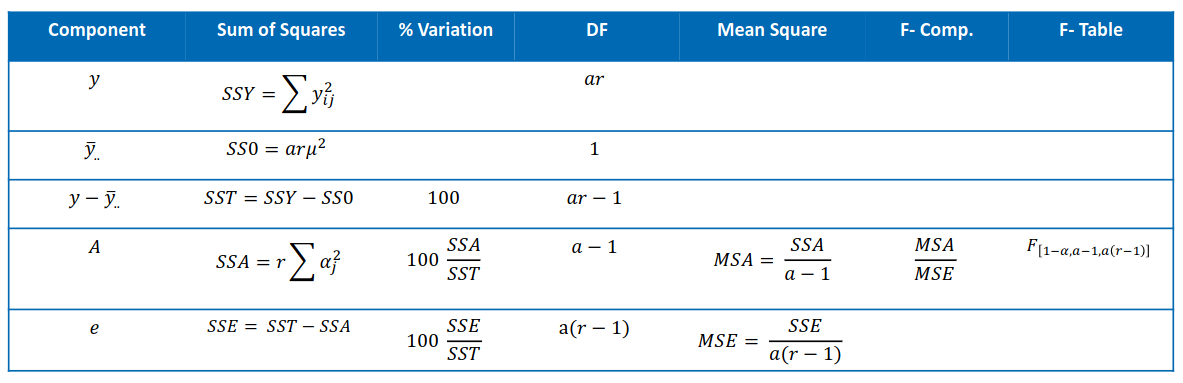
\includegraphics[width=0.95\textwidth]{figures/onefactor-anova.png}
  \end{center}
  \caption{Tabella ANOVA per design a singolo fattore}\label{fig:onefactor-anova}
\end{figure}

\subsection{Two factor design}
Usando due fattori categorici si parla di \textbf{\textit{2-factors design}}. In questo caso,
il modello risulta essere\footnote{in questa fase si stanno trascurando le ripetizioni}:

\subsubsection{2-factor experiments senza ripetizioni}
\paragraph{Modello e stima dei parametri}
In questo caso, si usa il modello mostrato in Equazione \ref{eq:2factor-model}.
\begin{equation}
  y_{ij} = \mu + \alpha_j + \beta_i + e_{ij}
  \label{eq:2factor-model}
\end{equation}

Analogamente al caso a singolo fattore, per la stima dei parametri si utilzzano i vincoli:
\begin{itemize}
  \item $\sum_{i=1}^b\beta_i = 0$
  \item $\sum_{j=1}^a\alpha_j = 0$
  \item $\sum_{j=1} e_{ij} = 0$
\end{itemize}

$\alpha_j$ si stima con la media della colonna $j-esima$:
\begin{align}
  \overline{y}_{.j} &= \mu + \frac{1}{a} \sum_j\alpha_j + \beta_i + \frac{1}{a}\sum_{j}e_{ij}\\
  &= \mu + \alpha_j \to \alpha_j = \overline{y}_{.j} - \overline{y}_{..}
\end{align}

\begin{align}
  \overline{y}_{i.} &= \mu + \frac{1}{a} \sum_j\alpha_j + \beta_i + \frac{1}{a}\sum_{j}e_{ij}\\
  &= \mu + \beta_i \to \beta_i = \overline{y}_{i.} - \overline{y}_{..}
\end{align}

\paragraph{Analisi degli errori}
L'obiettivo dell'analisi degli errori è sempre quello di stimare importanza e significatività. 
Definito l'errore come $e_{ij} = y_{ij} -  \hat{y}_{ij}$, si trova che, avendo stimato la 
risposta con il modello presentato in Equazione \ref{eq:2factor-model}:
\[
  e_{ij} = y_{ij} - \hat{y}_{ij} = y_{ij} - \mu - \alpha_j - \beta_i
\]
Quindi si può calcolare $SS_E$ come:
\[
  SS_E = \sum_{i=1}^b\sum_{j=1}^a e_{ij}^2
\]

L'allocazione della variazione si calcola effettuando la somma dei quadrati di ogni singolo
termine, ottenendo:
\[
  SS_Y = SS_0 + SS_A + SS_B + SS_E
\]
Ricordando che $SS_T = SS_Y - SS_0$, si ottiene che: 
\[
  SS_T = SS_A+SS_B+SS_E
\]

Definita quindi la significatività si passa ai valori quadratici medi. In un designa a due 
fattori si calcolano $MS_A$, $MS_B$ per capire la significatività dei singoli fattori
rispetto a $MS_E$. Analogamente al caso con un solo fattore si definiscono come:
\begin{itemize}
  \item $MS_A = \frac{SS_A}{a-1}$
  \item $MS_B = \frac{SS_B}{b-1}$
  \item $MS_E = \frac{SS_E}{(a-1)(b-1)}$
\end{itemize}

I gradi di libertà si ottengono con ragionamenti analoghi al caso a un fattore (la somma 
sulle righe di $B$ e sulle colonne di $A$ è nulla, mentre l'errore ha come gradi di libertà
il prodotto dei singoli fattori):
\[
  ab = 1 + (a-1) + (b-1) + (a-1)(b-1)
\]

Calcolati questi valori, si può eseguire l'$F$-test calcolando i due $f-value$ e comparandoli
con gli $\alpha$ percentili della distribuzione $f$. Quindi, valgono i segueni predicati:
\begin{enumerate}[label=(\alph*)] 
  \item Se $\frac{MS_A}{MS_E} > F_{[1-\alpha, a-1, (a-1)(b-1)]}$, allora $A$ è un fattore 
    significativo al $\alpha\cdot100$
  \item Se $\frac{MS_B}{MS_E} > F_{[1-\alpha, b-1, (a-1)(b-1)]}$, allora $B$ è un fattore 
    significativo al $\alpha\cdot100$
\end{enumerate}

In Figura \ref{fig:twofactor-anova}, è riportata la tabella ANOVA per esperimenti a due 
fattori senza ripetizioni
\begin{figure}
  \begin{center}
    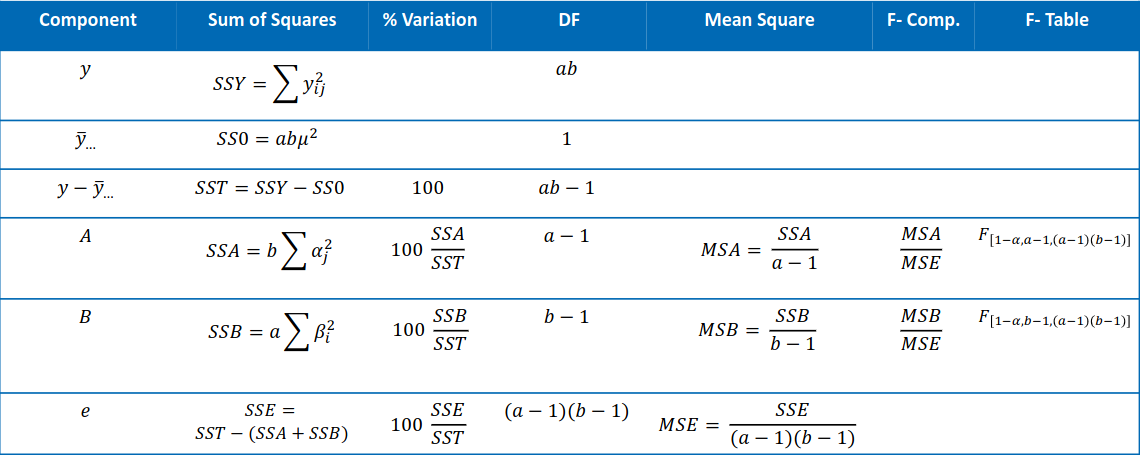
\includegraphics[width=.95\textwidth]{figures/twofactor-anova.png}
  \end{center}
  \caption{Tabella ANOVA per design a due fattori senza ripetizioni}
  \label{fig:twofactor-anova}
\end{figure}

\subsubsection{2-factor experiments con ripetizioni}
\paragraph{Modello e stima dei parametri}
In questo caso, si usa il modello mostrato in Equazione \ref{eq:2factor-model-rep}.
\begin{equation}
  y_{ijk} = \mu + \alpha_j + \beta_i + \gamma_{ij} + e_{ijk}
  \label{eq:2factor-model-rep}
\end{equation}
Per ogni esperimento si hanno $r$ ripetizioni.

Analogamente al caso senza ripetizioni, per la stima dei parametri si utilzzano i vincoli:
\begin{itemize}
  \item $\sum_{i=1}^b\beta_i = 0$: annullare gli effetti $B$ sulla riga $i-esima$
  \item $\sum_{j=1}^a\alpha_j = 0$: annullare gli effetti $A$ sulla colonna $j-esima$
  \item $\sum_{k=1} ^r e_{ijk} = 0$: annullare gli errori singoli esperimenti
\end{itemize}
A questi vincoli, si aggiungono quelli legati all'interazione $\gamma_{ij}$. In particolare,
le interazioni su ogni riga e su ogni colonna si annullano:
\[
  \sum_{j=1}^{a}\gamma_{ij} = 0 \; \forall i = 1,2,\dots, b
\]

\[
  \sum_{i=1}^{b}\gamma_{ij} = 0 \; \forall j = 1,2,\dots, a
\]

Analogamente al caso senza ripetizioni, gli effetti stimati dei fattori vengono stimati in 
base alle medie delle righe e delle colonne. In particolare, si definiscono le seguenti 
quantità:
\begin{itemize}
  \item $\overline{y}_{i..} = \frac{1}{jk} \sum_{j,k}y_{ijk} = \mu + \beta_i$
  \item $\overline{y}_{.j.} = \frac{1}{ik} \sum_{i,k}y_{ijk} = \mu + \alpha_j $
  \item $\overline{y}_{ij.} = \frac{1}{k} \sum_{k}y_{ijk} = \mu + \alpha_j + \beta_i + \gamma_{ij} $
  \item $\overline{y}_{...} = \frac{1}{ijk} \sum_{i,j,k}y_{ijk} = \mu $
\end{itemize}

Da cui si ricavano i parametri $\alpha_j, \beta_i, \mu, \gamma_{ij}$:
\begin{enumerate}
  \item $\alpha_j = \overline{y}_{.j.} - \overline{y}_{...}$
  \item $\beta_i = \overline{y}_{i..} - \overline{y}_{...}$
  \item $\gamma_{ij} = \overline{y}_{ij.} - \overline{y}_{i..} - \overline{y}_{.j.} + \overline{y}_{...}$
\end{enumerate}

\paragraph{Analisi degli errori}
L'obiettivo dell'analisi degli errori è sempre quello di stimare importanza e significatività. 
Definito l'errore come $e_{ijk} = y_{ijk} -  \hat{y}_{ijk}$, si trova che, avendo stimato la 
risposta con il modello presentato in Equazione \ref{eq:2factor-model-rep}:
\[
  e_{ij} = y_{ij} - \hat{y}_{ij} = y_{ij} - \mu - \alpha_j - \beta_i
\]
Quindi si può calcolare $SS_E$ come:
\[
  SS_E = \sum_{i=1}^b\sum_{j=1}^a e_{ij}^2
\]

L'allocazione della variazione si calcola effettuando la somma dei quadrati di ogni singolo
termine, ottenendo:
\[
  SS_Y = SS_0 + SS_A + SS_{AB} + SS_E
\]
Ricordando che $SS_T = SS_Y - SS_0$, si ottiene che: 
\[
  SS_T = SS_A+SS_B+ SS_{AB} + SS_E
\]

Definita quindi la significatività si passa ai valori quadratici medi. In un designa a due 
fattori si calcolano $MS_A$, $MS_B$ per capire la significatività dei singoli fattori
rispetto a $MS_E$. Analogamente al caso con un solo fattore si definiscono come:
\begin{itemize}
  \item $MS_A = \frac{SS_A}{a-1}$
  \item $MS_B = \frac{SS_B}{b-1}$
  \item $MS_AB = \frac{SS_AB}{(a-1)(b-1)}$
  \item $MS_E = \frac{SS_E}{ab(r-1)}$
\end{itemize}

I gradi di libertà si ottengono con ragionamenti analoghi al caso a un fattore (la somma 
sulle righe di $B$ e sulle colonne di $A$ è nulla, mentre l'errore ha come gradi di libertà
il prodotto dei singoli fattori):
\[
  ab = 1 + (a-1) + (b-1) + (a-1)(b-1) + ab(r-1)
\]

Calcolati questi valori, si può eseguire l'$F$-test calcolando i due $f-value$ e comparandoli
con gli $\alpha$ percentili della distribuzione $f$. Quindi, valgono i segueni predicati:
\begin{enumerate}[label=(\alph*)] 
  \item Se $\frac{MS_A}{MS_E} > F_{[1-\alpha, a-1, ab(r-1)]}$, allora $A$ è un fattore 
    significativo al $\alpha\cdot100$
  \item Se $\frac{MS_B}{MS_E} > F_{[1-\alpha, b-1, ab(r-1)]}$, allora $B$ è un fattore 
    significativo al $\alpha\cdot100$
  \item Se $\frac{MS_{AB}}{MS_E} > F_{[1-\alpha, (a-1)(b-1), ab(r-1)]}$, allora l'interazione
    è significativa al $\alpha\cdot100$
\end{enumerate}

In Figura \ref{fig:twofactor-rep-anova}, è riportata la tabella ANOVA per esperimenti a
due fattori con $r$ ripetizioni.
\begin{figure}
  \begin{center}
    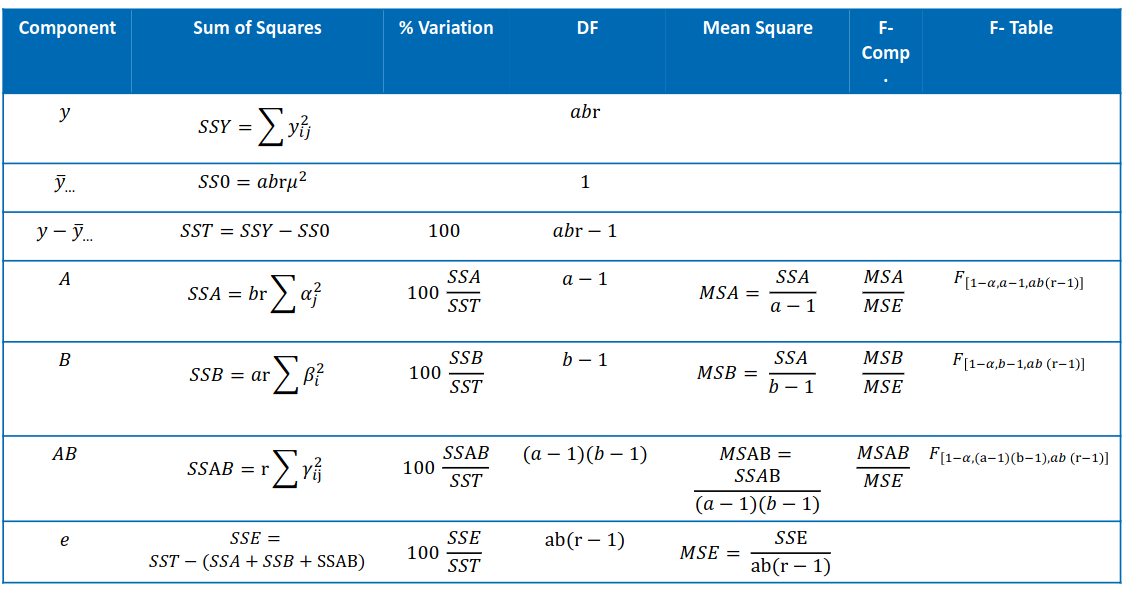
\includegraphics[width=.95\textwidth]{figures/twofactor-rep-anova.png}
  \end{center}
  \caption{Tabella ANOVA per design a due fattori con ripetizioni}
  \label{fig:twofactor-rep-anova}
\end{figure}

\subsection{Riepilogo}
I modelli visti, valgono nell'ipotesi di normalità e omoschedasticità dei residui. In 
tal caso infatti è possibile effettuare test parametrici come l'$F-Test$, altrimenti bisogna
seguire la tabella in Figura \ref{fig:recap-doe}. 

\begin{figure}
  \begin{center}
    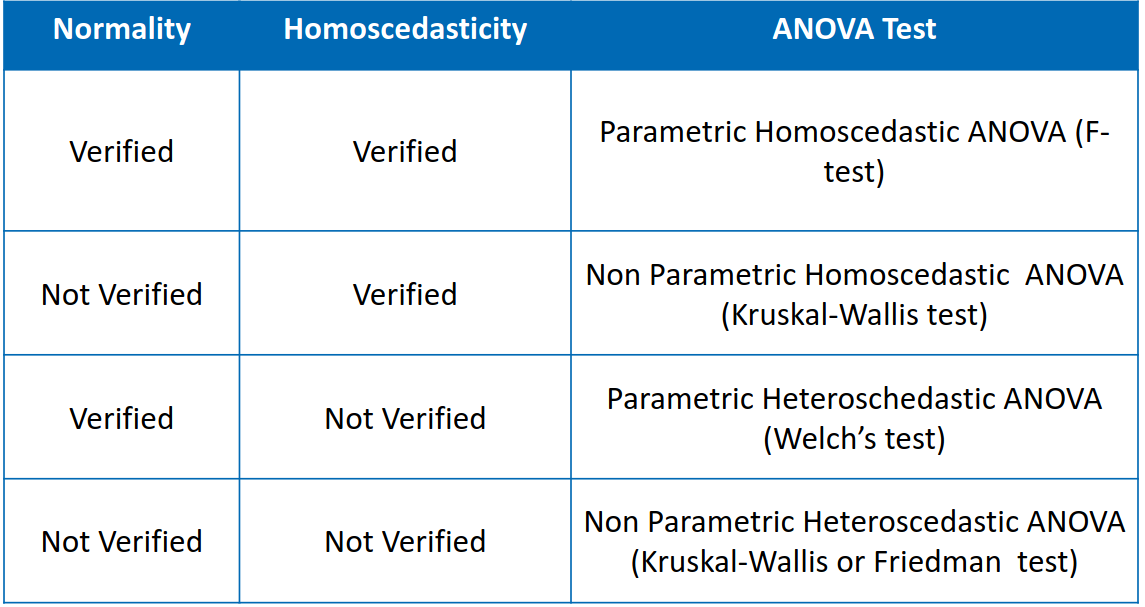
\includegraphics[width=.95\textwidth]{figures/recap-doe.png}
  \end{center}
  \caption{Tabella riepilogo generale per Design of Experiment}
  \label{fig:recap-doe}
\end{figure}

\clearpage
\section{Dependability}
In questa fase del corso, si fa riferimento a sistemi detti critici. Un sistema può essere
definito critico se il fallimento dello stesso comporta danni catastrofici in un determinato 
ambito. Principalmente, si parla di:
\begin{itemize}
  \item \textbf{Business critical}: sistemi il cui fallimento porta a perdite economiche;
  \item \textbf{Safety critical}: sistemi il cui fallimento porta a perdite di vite umane;
  \item \textbf{Mission critical}: sistemi il cui fallimento porta a mancare un obiettivo
    cruciale;
\end{itemize}

Si è interessati a studiare le caratteristiche di dependability per progettare
sistemi sicuri. Ma cosa è la \textit{dependability}?

\textbf{Dependability} è un termine ombrello (Figura \ref{fig:dep-tree}) che viene 
utilizzato per indicare attributi quali: integrità (\textbf{\textit{integrity}}, 
manutenibilità \textbf{\textit{mantainability }}, sicurezza \textbf{\textit{safety and 
security}}, disponibilità (\textbf{\textit{availability}}) e \textbf{\textit{reliability}} e
può essere  applicato a un intero sistema \footnote{In questo contesto con la parola sistema
ci si può riferire a a un singolo modulo, a un sottosistema più complicato a un componente
\dots} coinvolgendo la parte hardware, software e infrastrutturale.

\begin{figure}
  \begin{center}
    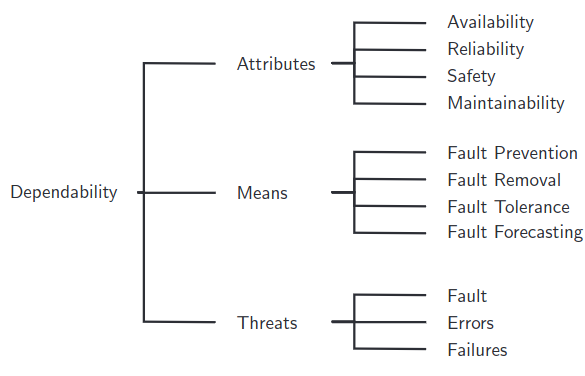
\includegraphics[width=.7\textwidth]{figures/dep-tree.png}
  \end{center}
  \caption{Termini inclusi con dependability}\label{fig:dep-tree}
\end{figure}


\subsection{Definizioni}
Di seguito sono riportate le definizioni fondamentali per lo studio della dependability.

\paragraph{Sistema} Un sistema indica un entità che può interagire con altre entità. 
Con entità si può far riferimento sia ad altri sistemi (hardware o software), umani e 
fenomeni provenienti dal mondo fisico. Ogni sistema ha un'\textbf{interfaccia} che espone 
come separazione tra esso e il mondo esterno.

\paragraph{Servizio}Un servizio è il comportamento del sistema percepito dai propri utenti.
Un utente è un altro sistema che riceve i servizi da un provider. Un servizio è corretto se
rispetta le sue specifiche.


\paragraph{Fault $\to$ error $\to$ failure chain}Quando un sistema non si comporta secondo 
la sua specifica si dice che ci si trova di fronte ad un \textbf{fallimento}
(\textbf{\textit{failure}}). Un fallimento è la \textbf{propagazione} all'utente di una
condizione di \textbf{errore}(\textbf{\textit{error}}). In particolare, un errore è
l'attivazione di un \textbf{\textit{fault}}\footnote{Un fault può essere visto come un bug
nel codice sorgente che viene attivato solo se si verifica una determinata condizione
portando ad un errore.} 
Un \textit{fault} non attivato si dice \textbf{dormiente} e viene innescato 
da un \textbf{pattern di attivazione}. In Figura \ref{fig:dep-fault-error-failure-chain},
è mostrata la catena di attivazione di un fault e di propagazione degli errori.

\begin{figure}
  \begin{center}
    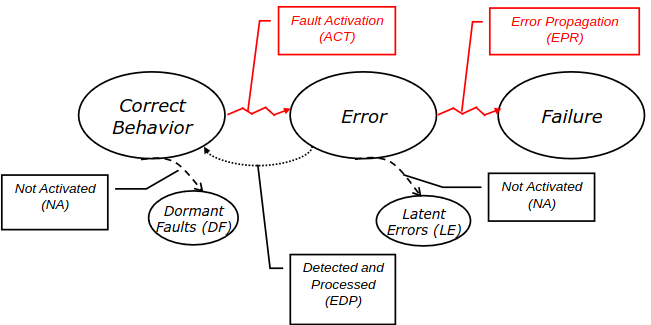
\includegraphics[width=.8\textwidth]{figures/dep-fault-error-failure.png}
  \end{center}
  \caption{Esempio di \textit{fault-error-failure chain}}
  \label{fig:dep-fault-error-failure-chain}
\end{figure}


Quindi, a valle di un fallimento bisogna risalire al fault che ha generato 
l'errore. In generale, sono vere le seguenti affermazioni:
\begin{itemize}
  \item Ad un singolo \textit{fault} possono essere collegati più errori;
  \item Non è detto che ogni errore si manifesti all'utente sottoforma di fallimento, ma 
    può restare in una condizione \textbf{mascherata};
\end{itemize}

\paragraph{Classificazione di fault}In letteratura, i fault vengono analizzati da $4$ 
prospettive differenti:
\begin{enumerate}
  \item Cause: le cause di un fault possono essere umane o fisiche. I primi possono essere 
    dovuti alla fase di progettazione, all'analisi non accurata di uno scenario, Difetti 
    di procedure operative ecc; quelli fisici sono semplicemente dovuti a guasti di  
    componenti elettroniche;
  \item Persistenza: un fault può essere \textbf{permanente} (la condizione del sistema
    dopo il verificarsi dell'evento è stabile e continua), \textbf{transiente} (il fault
    modifica la condizione del sistema solo per un breve periodo), \textbf{intermittente}
    (il fault si attiva in maniera occasionale a causa di instabilità o nell'hardware o nel 
    software);
  \item Intenzionalità: un fault può essere stato attivato volontariamente per creare danno
    (\textbf{malevolo}) o senza volontà ostili;
  \item Origini: un fault può essere dovuto allo stato interno del sistema in esame o 
    esterne;
\end{enumerate}

\paragraph{Sistemi riparabili e non riparabili} Un sistema può essere in due stati: 
\textbf{up} (in funzione) o \textbf{down} (fallimento). Un sistema riparabile può tornare 
nella condizione \textit{up} dopo che è passato in \textbf{\textit{down}} (Figura
\ref{fig:dep-up-down}), mentre uno non riparabile una volta fallito rimane nella sua 
condizione \textit{down}.

\begin{figure}
  \begin{center}
    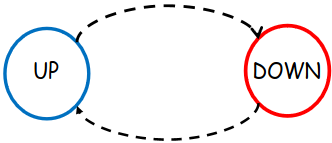
\includegraphics[width=.4\textwidth]{figures/dep-up-down.png}
  \end{center}
  \caption{Diagramma degli stati per un sistema riparabile}\label{fig:dep-up-down}
\end{figure}

\paragraph{Bathub curve}Solitamente la distribuzione esponenziale è usata per caratterizzate
i failure di un sistema. Infatti, questa esprime l'indipendenza dei fallimenti e porta ad  
essere in un sistema \textbf{\textit{memoryless}}. I costruttori sfruttano queste 
distribuzioni per creare curve come quella in Figura per caratterizzare il tempo di vita
di un dispositivo. La curva in Figura \ref{fig:dep-bathub} è detta \textit{bathub curve}
\footnote{Il nome deriva dalla forma di una vasca da bagno} e può essere suddivisa in tre
regioni dette epoche:
\begin{enumerate}
  \item Infant mortality: quella più a sinistra. I dispositivi sono in fase prototipale e 
    quindi presentano un tasso di errori molto alto che decresce fino ad entrare nella
    fase successiva;
  \item Normal lifetime: in questa fase il tasso di fallimenti è costante;
  \item Wearout period: il dispositivo raggiunge il fine vita e si osserva una crescita 
    esponenziale del tasso dei fallimenti;
\end{enumerate}

\begin{figure}
  \begin{center}
    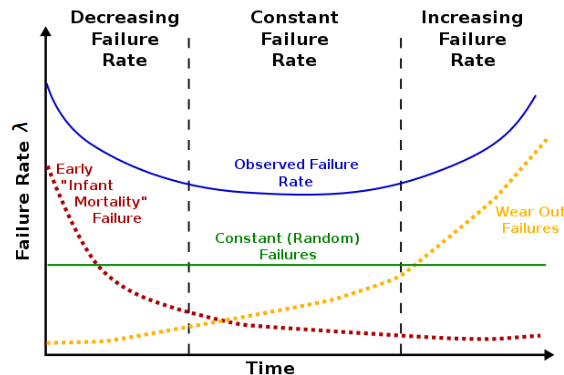
\includegraphics[width=.7\textwidth]{figures/dep-bathub.png}
  \end{center}
  \caption{Esempio di bathub curve}\label{fig:dep-bathub}
\end{figure}


\subsubsection{Reliability di sistemi non riparabili}
I sistemi non riparabili possono modellare il loro tempo al fallimento (\textbf{\textit{time 
to failure}}) con una variabile aleatoria $X$. L'Equazione \ref{eq:unrealiability}
indica $CDF$ di $X$ e rappresenta l'\textbf{\textit{unrealiability}} del componente:
\begin{equation}
  F_x(t) = P{X < t} 
  \label{eq:unrealiability}
\end{equation}
In quanto $CDF$ di una variabile aleatoria, questa gode delle seguenti proprietà:

\begin{cases}
  F_X(0) \geq 0 \\
  \lim_{t\to \infty} F_X(t) = 1\\ 
  F_X(t) \text{ è non decrecente in t}
\end{cases}

Intuitivamente, la reliability è la funzione complementare all'unreliability ovvero la 
probabilità che il sistema operi correttamente entro un intervallo $[0, t]$ dove con $t$ 
si indica il \textbf{tempo di missione}. La reliability risulta essere:
\begin{equation}
  R_X(t) = P(X > t) = 1 - F_X(t)
  \label{eq:reliability}
\end{equation}
Data la definizione in Equazione \ref{eq:reliability}, valgono le seguenti proprietà:

\begin{cases}
  R_X(0) = 1 \\
  \lim_{t\to \infty} R_X(t) = 0\\ 
  R_X(t) \text{ è non crecente in t}
\end{cases}

Gli andamenti di $F_X(t)$ e $R_X(t)$ sono riportati in Figura \ref{fig:reliability_vs_unrel}.

\begin{figure}
  \begin{center}
    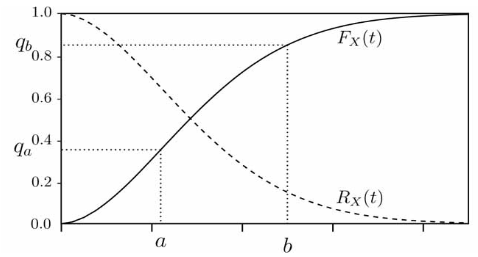
\includegraphics[width=.6\textwidth]{figures/dep-rel_vs_unrel.png}
  \end{center}
  \caption{Tipiche curve della funzione di reliability e quella di unreliability}
  \label{fig:reliability_vs_unrel}
\end{figure}

Spesso di $X$ è nota la $pdf = f_X(t)$. Pertanto, ricordando la definizione $R_X(t)$ e quella
di $pdf$ si ottiene che:
\[
  f_X(t) = \frac{dF_x(t)}{dt} \to f_X(t) = - \frac{dR_X(t)}{dt}
\]
Quindi è possibile calcolare la probabilità che ci sia un fallimento in un intervallo $[a,b]$a
applicando la relazione in Equazione \ref{eq:prob-between}. 

\begin{equation}
  P(a \leq X \leq b) = \int_a^b f_X(t) \,dt = F_X(b) - F_X(a)
  \label{eq:prob-between}
\end{equation}

\subsubsection{Reliability di sistemi riparabili}
Un sistema riparabile può essere ripristinato in uno stato operativo dopo un fallimento. In 
questo caso, il comportamento del sistema dipende da come viene recuperato e dal tempo 
impiegato per effettuare la riparazione. Per questo motivo, l'andamento del sistema risulta
essere quello \ref{fig:repairable}.

\begin{figure}
  \begin{center}
    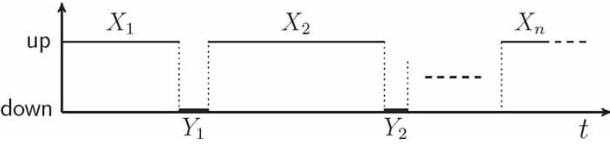
\includegraphics[width=.75\textwidth]{figures/dep-repairable.png}
  \end{center}
  \caption{Andamento stato operativo di un sistema riparabile}
  \label{fig:repairable}
\end{figure}

\subsubsection{Metriche per la dependability}

In base alla situazione e al tipo di sistema si possono costruire metriche utili per il 
calcolo della dependability. Le principali metriche sono indicate in Figura \ref
{fig:dep-metrics.png}

\begin{figure}
  \begin{center}
    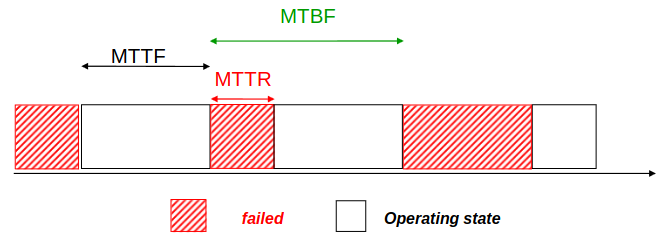
\includegraphics[width=0.95\textwidth]{figures/dep-metrics.png}
  \end{center}
  \caption{Metriche principali per la dependability}\label{fig:dep-metrics.png}
\end{figure}


\paragraph{Reliability}La reliability è una misura della continuità del servizio offerto e 
si indica con $R(t)$. Il valore atteso di questo valore è detto \textbf{MTTF}
(\textbf{\textit{Mean time to failure}}) ed è definito come:

\begin{equation}
  MTTF = E[X] = \int_0^\infty tf_X(t)\,dt = \int_0^\infty R_X(t)\,dt
  \label{eq:mttf}
\end{equation}

Quindi assumendo che la distribuzione dei fault è esponenziale, si ottiene che $pdf = f_x(t)=
\lambda e^{-\lamda t}$, $F_X(t) = 1 - e^{-\lamda t}$. Quindi $R_X(t) = e^{-\lambda t}$ e,
applicando l'Equazione \ref{eq:mttf}, si ottiene $MTTF = \frac{1}{\lambda}$. Il parametro
$\lambda$ è detto \textbf{\textit{failure rate}}.

\paragraph{Mantainability} Si tratta di una misura che indica la probabilità che 
il sistema sia riparato entro un tempo $t$. Si indica con $M(t)$. Il valore atteso di questa
misura è l'MTTR (\textbf{\textit{mean time to repair}}).

\paragraph{Availability} Misura che indica la consegna effettiva del servizio in relazione
alle interruzioni in un sistema riparabile. Formalmente, $A(t)$ è la probabilità che il 
servizio funzioni correttamente all'istante $t$. Il suo valore atteso è definito come:
\[
  A = \frac{MTTF}{MTTF + MTTR}
\]

In particolare, si definiscono $A(t) = P\{\text{unità up al tempo t}\}$ e $U(t) = P\{
  \text{unità down al tempo t}\}$. Ovviamente per la proprietà di normalità vale:
\[
  A(t) + U(t) = 1
\]

In ogni caso, per un sistema riparabile spesso ha più senso parlare di MTBF (
\textbf{\textit{mean time between failures}}) che può essere associato a MTTF se il tempo 
per la riparazione è trascurabile. 

\[
  MTTF \approx MTBF = \int_0^\infty R(t)\, dt
\]
Quando questo non può essere trascurato bisogna sommare le due quantità:
\[
  MTBF = MTTF + MTTR
\]

\paragraph{Safety} Misura la probabilità $S(t)$ che nessun evento catastrofico si verifichi
nell'intervallo $(0,t)$. Il suo valore medio è detto $MTTCF$ (\textbf{\textit{mean time to 
catastrophic failure}}. 

La \textit{safety} è espressa come un livello di accettazione delle perdite. Il valore 
atteso delle perdite per unità di tempo è il \textbf{\textit{rischio}} definito come:
\begin{equation*}
  Risk = \sum_i P(\text{si verifica l'incidente $i$}) \cdot cost(\text{incidente $i$})
\end{equation*}

\subsection{Dependable computing}
Data le definizioni principali di \textit{dependability}, si voglio costruire dei modelli
per stimare quest'attributo in presenza di sistemi complessi composti da più componenti. 
Si parla di \textbf{\textit{dependable computing}} quando ci si riferisce ad un esecuzione 
corretta di una funzione anche in presenza di guasti. In fase di progettazione, esistono
due approcci:
\begin{itemize}
  \item \textbf{\textit{Fault avoidance}}: consiste nel ridurre la 
    possibilità di fallimento di un sistema. Questa tecnica non ammete la presenza di fault e,
    pertanto risulta molto difficile da realizzare. Infatti, pensando alla classificazione
    dei fault si ricorda che alcuni di questi sono dovuti a fattori esterni.
  \item \textbf{\textit{Fault tolerance}}: sfrutta tecniche di ridondanza per rendere il 
    sistema più affidabile;
\end{itemize}


\paragraph{Duplicazione}La duplicazione è il più semplice esempio di ridondanza. Questa 
tecnica effettua l'attività di \textit{fault detection} e consiste nel installare $2$ 
copie identitche dello stesso componente (Figura \ref{fig:dep-duplication}). 
Entrambe le copie sono collegate ad un comparatore e ricevono lo stesso input. 
Il comparatore confronta le uscite dei due sistemi: se sono diverse allora c'è stato un 
fault.

\begin{figure}
  \begin{center}
    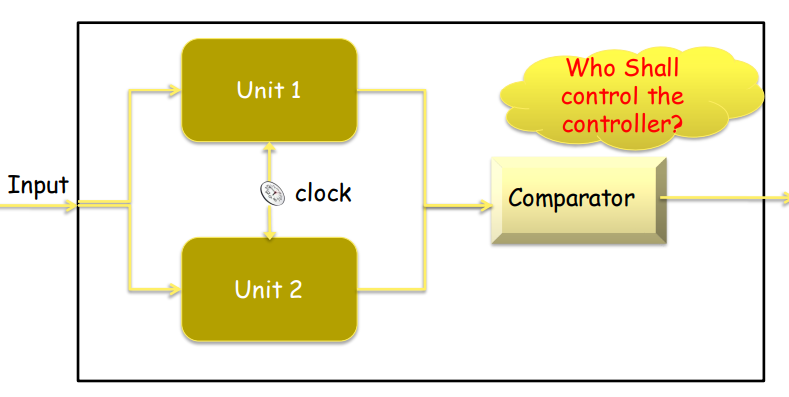
\includegraphics[width=.7\textwidth]{figures/dep-dual-redundancy.png}
  \end{center}
  \caption{Esempio di ridondanza con $2$ copie}\label{fig:dep-duplication}
\end{figure}

Questa tecnica individua correttamente tutti i guasti singoli, ma non quelli di modo comune:
se entrambi i dispositivi falliscono allo stesso modo le uscite saranno uguali (sebbene 
errate) e il comparatore non rileverà nulla. Inoltre, il comparatore deve essere almeno
un ordine di grandezza più affidabile dei singoli sistemi e si dice costituisce un 
\textbf{\textit{single point of failure}}. 

Formalmente, volendo calcolare la reliability di questo sistema bisogna trovare:
\[
  F_d(t) = P(X_1 \leq t\, or\, X_2 \leq t) = 1 - P(X-1 > t\, and\, X_2 > t ) = 1 - 
  [(1-F_1(t)) (1-F_2(t))]
\]
Passando a $pdf$ e assumento i guasti esponenziali con failure rate $\lambda_1, \lambda_2$:
\[
  R_D(t) = R_1(t) R_2(t) \to R_D(t) = e^{-(\lambda_1 + \lambda_2)t}
\]

Quindi la reliability trovata ha un $MTTF = \frac{1}{\lambda_1 + \lambda_2}$ che, mostrato 
in Figura \ref{fig:redundancy_vs_simplex}, che è minore del sistema con un solo componente
(detto \textbf{\textit{simplex}}).

\begin{figure}
  \begin{center}
    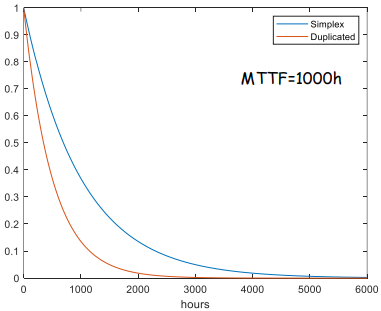
\includegraphics[width=.6\textwidth]{figures/dep-redundancy_vs_simplex.png}
  \end{center}
  \caption{Un sistema ridondato ha un MTTF inferiore a quello simplex}
  \label{fig:redundancy_vs_simplex}
\end{figure}

\subsection{Modelli combinatori per la fault tolerance}
Fatte alcune assunzioni semplificative, nel mondo industriale si preferisce utilizzare 
approcci quantitativi mediante modelli analitici per stimare in una prima istanza la 
dependability di un sistema. I modelli matematici adottati sono combinatori (senza spazio 
di stato) per forniscono una stima accettabile della denpendability.

In questi modelli, ogni componente può essere associata:
\begin{itemize}
  \item Una probabilità di fallimento;
  \item Un tasso di fallimento;
  \item Una $pdf$ del tempo al fallimento;
  \item Una unvailability a regime e istantanea;
\end{itemize}

\paragraph{Assunzioni}Per utilizzare modelli combinatori è necessario che tutti i componenti
del sistema siano \textbf{indipendenti}. Inoltre, deve valere che:
\begin{itemize}
  \item I fallimenti sono tra loro indipendenti;
  \item I fallimenti sono di tipo permanente: quando un componente fallisce permane nello 
    stato errato;
  \item Un sistema è funzionante solo se funzionano un certo numero di componenti al suo 
    interno;
  \item Le unità analizzate si assumono non riparabili;
\end{itemize}

\subsubsection{RBD - Reliability Block Diagram}
Questa tecnica prevede una visualizzazione del sistema attraverso uno schema a blocchi in 
cui ci si focalizza sul fatto che il sistema funzioni al tempo $t$. Bisogna quindi capire 
come varia la reliability dei diversi collegamenti. I principali sono il collegamento in 
serie e quello in parallelo. Questi diagrammi a blocchi sono appunto detti 
\textbf{Reliability Block Diagram}.

\paragraph{Collegamento in serie}Questo collegamento prevede la cascata tra $n$ blocchi 
(Figura \ref{fig:series-def}). Si sta dicendo che questi devono funzionare tutti affinchè 
il sistema non fallisca. La probabilità che il sistema $S$ funzioni è data da:
\begin{align}
  P\{S\} &= P\{E_1 \land E_2 \land \dots \land E_n\}\\ 
  &= \prod_{i=1}^nP\{E_i\}
\end{align}
in cui si è assunto che $E_1,E_2,\dots,E_n$ siano indipendenti tra loro.

\begin{figure}
  \begin{center}
    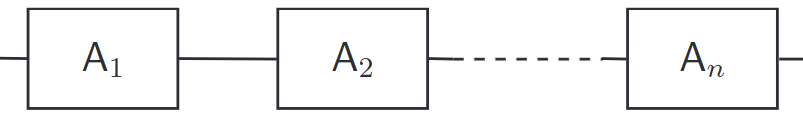
\includegraphics[width=.7\textwidth]{figures/dep-series.png}
  \end{center}
  \caption{Sistemi collegati in serie}\label{fig:series-def}
\end{figure}

Questo vuol dire che la reliability risultante $R_s$ è:
\begin{equation}
  R_s(t) = \prod_{i=1}^n R_i(t)
  \label{eq:series-def}
\end{equation}

Il failure rate aumenta al crescere del numero dei componenti del sistema ed è sempre minore
del componente meno affidabile del sistema:
\[
  R_s < \min\{R_1, R_2, \dots, R_n\} \implies 0 \leq MTTF \leq \min\{MTTF_i\}
\]

\paragraph{Blocchi in serie: caso esponenziale}Assumendo esponenziali la distribuzione 
dei fallimenti per ogni componente, secondo l'Equazione \ref{eq:series-def}, si ottiene che:
\[
  R_s(t) = e^{-(\sum_{i=1}^n \lambda_i)t}
\]
dove con $\lambda_i$ si è indicato il \textit{failure rate} del componente $i-esimo$.

Studiando l'MTTF del sistema risultante si nota che questo equivale a: 
\[
  MTTF = \frac{1}{\lambda_s} = \frac{1}{\sum_{i=1}^n\lambda_i}
\]

\paragraph{Blocchi in parallelo} In questo caso, bisogna far riferimento a sistemi 
ridondati che collegano all'uscita un elemento quando si guasta uno di questi. In Figura
\ref{fig:parallel}, sono collegati $n$ blocchi in parallelo. Affinchè il sistema funzioni 
almeno uno di questi deve essere operativo.

\begin{figure}
  \begin{center}
    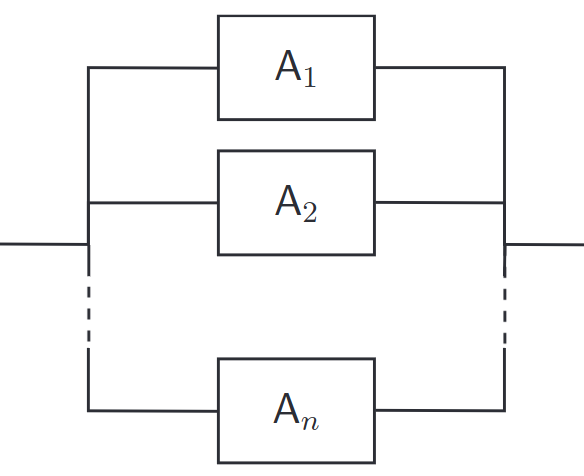
\includegraphics[width=.6\textwidth]{figures/dep-parallel.png}
  \end{center}
  \caption{Blocchi collegati in parallelo}\label{fig:parallel}
\end{figure}

Quindi, definiti gli $\overline{E}_i = \text{componente i-esimo è fallito}$ e $\overline{E}_p
=\text{sistema parallelo è fallito}$, si ottiene che il parallelo fallisce se falliscono 
tutti i suoi componenti:
\begin{align}
  P\{\overline{E}_p\} &= P\{\overline{E}_1 \land \overline{E}_2 \land \dots \land 
  \overline{E}_n\}\\
  &= \prod_{i=1}^nP\{\overline{E}_i\}
\end{align}
Dovendo funzionare almeno un componente, allora basta calcolare:
\[
  P\{\text{almeno 1 funziona}\} = 1 - \prod_{i=1}^n P\{\overline{E}_i\}
\]

Quindi, detta $R_i(t)$ la reliability del componente $i-esimo$ (probabilità che $i$ 
non funzioni), si ottiene che $F_i(t) = 1 - R_i(t)$ (probabilità che $i$ non funzioni), 
si può calcolare $F_{par}$ come:
\begin{equation}
  F_{par} = F_1F_2\dots F_n = (1-R_1)(1-R_2)\dots(1_R_n) = \prod_{i=1}^n(1- R_i)
  \label{eq:unrel-parall}
\end{equation}
Dalla Equazione \ref{eq:unrel-parall}, si calcola $R_{par}$ come:
\[
  R_{par} = 1 - F_{par} = 1 - \prod_{i=1}^n(1-R_i)
\]

\paragraph{Sistemi non ricoduncibili a serie-parallelo: teorema dell'upper bound} 
Quando un sistema non è ricondudcile a serie-parallelo, la reliability non può essere stimata
facilmente. Tuttavia, esiste il teorema dell'\textbf{\textit{upper bound}} che consente di
stimare un limite superiore alla relability del sistema. Il teorema fa riferimento ai
\textbf{\textit{success path}} di un RBD. Un success path consiste in una serie di
attraversamenti tra l'ingresso e l'uscita di un sistema che lo lasciano in uno stato 
operativo. 

Ad esempio, in Figura \ref{fig:dep-noseries-parallel} è riportato l'esempio di un sistema non 
riducibile con serie e parallelo. La strategia dei \textit{success path} consiste nell'
enumerare tutti questi percorsi in modo tale da creare un parallelo di serie da poter trattare
in maniera classica. Quindi, trovati $n$ percorsi, si creerà un sistema equivalmente con un 
parallelo composto da $n$ elementi, ciascuno dei quali sarà la serie dei blocchi attraversati 
dal singolo percorso (Figura \ref{fig:dep-success-path}).

\begin{figure}
  \centering
  \begin{subfigure}{0.5\textwidth}
    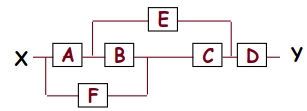
\includegraphics[width=.95\textwidth]{figures/dep-noseries-parallel.png}
    \caption{Sistema no serie-parallelo}
    \label{fig:dep-noseries-parallel}
  \end{subfigure}\hfil
  \begin{subfigure}{0.5\textwidth}
    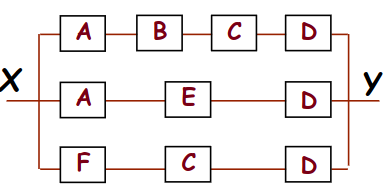
\includegraphics[width=.8\textwidth]{figures/dep-success-path.png}
    \caption{Enumerazione dei \textit{success path}}
    \label{fig:dep-success-path}
  \end{subfigure}
  \caption{\ref{fig:dep-noseries-parallel} Sistema no serie parallelo. 
  \ref{fig:dep-success-path} Sistema ottenuto attraverso l'enumerazione dei success path}
\end{figure}

Il teorema dell'upper bound afferma che:
\[
  R_{sys} \leq 1 - \prod_{i=1}^n(1- R_{i})
\]
dove con $i$ si indicano i success path. La relazione di disuguaglianza può essere
trasformata in uguaglianza se i path trovati risultano essere indpendenti.

\paragraph{Sistemi non ricoduncibili a serie-parallelo: regola di Bayes} In presenza di 
sistemi non banali, è possibile utilizzare la tecnica del conditioning per trovare la 
reliability del sistema. Questa tecnica consiste nello sfruttare la legge della probabilità 
totale secondo cui:
\[
  P(A) = \sum_{i=1}^n P\{A|B_i\}P\{B_i\}
\]
Nel caso degli RBD, si può assumere un componente una volta guasto e una volta non guasto e 
combinare gli effetti dei due sistemi equivalenti. Ad esempio, dato un sistema con un modulo
$m$ si dimostra che:
\[
  R_{sys} = R_mP\{\text{sistema funziona}|\text{m funziona}\} + 
  (1-R_m)P\{\text{sistema funziona}|\text{m non funziona}\} 
\]
Questa tecnica può essere applicata in maniera iterativa fino ad ottenere un sistema semplice
risolvivile con serie e parallelo.

\subsubsection{Sistemi $k$ su $n$} la fault tolerance può essere ottenuta con un sistema 
n-modulare ridondato. Questa tecnica consiste nel ridondare un componente abbastanza 
informazioni da mascherare un fault (\textbf{\textit{fault masking}}). Sostanzialente, come 
mostrato in Figura \ref{fig:tmr}, si collegano le unità ridondate a un
\textbf{\textit{voter}}. L'uscita sarà quella proposta da almeno $k$ su $n$ componenti. 
Infatti, questi sistemi ridondati 

\begin{figure}
  \begin{center}
    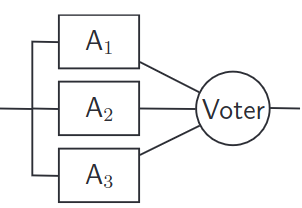
\includegraphics[width=.5\textwidth]{figures/dep-tmr.png}
  \end{center}
  \caption{Esempio di ridondanza n-modulare con $n=3$}\label{fig:tmr}
\end{figure}

L'esempio in Figura \ref{fig:tmr} prende il nome di \textbf{TMR} (\textit{Three modular 
redundancy}) e sono una classe particolare di sistemi che hanno bisogno di $2/3$ voti 
per mascheare un fault.

In generale, la reliability di un sistema $M$ su $N$ si calcola sommando tutte le
combinazioni in cui si rompono al più $N-M$ elementi:
\begin{equation}
  R_{MN} = \sum_{i=1}^{N-M}\binom{N}{i}R_m^{n-i}(1-R_m)^i
  \label{eq:tmr}
\end{equation}

Nel caso particolare del TMR, la relazione in Equazione \ref{eq:tmr} diventa 
\[
  R_{TMR} = R_m^3 + \binom{3}{2}R^2(1-R_m)
\]
L'Equazione \ref{eq:tmr} assume che il voter abbia una reliability ideale, ma in realtà
può avere dei fault ed è semplicemente un altro componente in cascata: 
\[
  R_{TMRV} = R_v(R_m^3 + \binom{3}{2}R^2(1-R_m))
\]
Il voter costituisce un singolo point of failure del sistema, e pertanto, esistono 
configurazioni con più voter. Ad esempio, in Figura \ref{fig:tmr3v}, è mostrato un TMR 
con $3$ voter.

\begin{figure}
  \begin{center}
    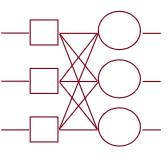
\includegraphics[width=.2\textwidth]{figures/dep-tmr3v.png}
  \end{center}
  \caption{Esempio di TMR con $3$ voter}\label{fig:tmr3v}
\end{figure}

Si può pensare di migliorare la reliability di un sistema applicando il TMR a tutti i blocchi
in cascata, ottenendo un sistema come in Figura \ref{}. La reliability di 
tale sistema risulta:
\[
  R_{cascade} = \left(R_v\left(R^3 + \binom{3}{2}R^2_m(1-R_m)\right)\right)^n
\]
\paragraph{TMR vs. Simplex} È stato già mostrato quando si è parlato di semplice ridondanza
la reliability di un sistema tende a peggiorare quando si aggiungono componenti al sistema. 
Tuttavia, strategie come TMR sono ampiamente utilizzate all'interno dei sistemi reali. 
Perchè? Osseervando il confronto in Figura \ref{fig:tmr-vs-simplex}, si evince che per un
tempo di missionebasso la reliability del TMR risulta molto più alta del sistema simplex.
Ciò vuol dire che i componenti extra aumentano la tolleranza ai fault ma solo per un preve
periodo. Quello che avviene in Figura \ref{fig:tmr-vs-simplex}, può essere riassunto in 
\begin{equation*}
  \begin{cases}
    R_{TMR}(t) \geq R_{simplex}(t), &\text{ if } t<t_0\\
    R_{TMR}(t) \leq R_{simplex}(t), &\text{ if } t>t_0
  \end{cases} 
\end{equation*}

\begin{figure}
  \begin{center}
    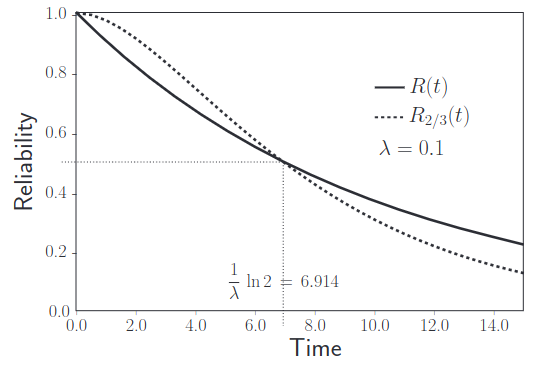
\includegraphics[width=.6\textwidth]{figures/dep-tmr-vs-simplex.png}
  \end{center}
  \caption{Confronto tra reliability di un TMR e quella di un simplex}
  \label{fig:tmr-vs-simplex}
\end{figure}

Infatti, volendo guardare solo l'MTTF, si nota che un simplex ha un MTTF migliore di un TMR,
calcolato in Equazione \ref{eq:mttf-tmr} assumendo la distribuzione dei guasti esponenziale
con failure rate $\lambda$.

\begin{align}
  MTTF_{TMR} &= \int_0^\infty R_{TMR}(t)\,dt \\ 
  &= \int_0^\infty e^{-3\lambda t} + \binom{3}{2}  e^{-2\lambda t}(1-e^{-\lambda t})\,dt \\ 
  &= \int_0^\infty e^{-3\lambda t} + 3e^{-2\lambda t}-3^{-3\lambda t}\,dt\\
  &= \int_0^\infty -2e^{-3\lambda t} + 3e^{-2\lambda t}\,dt\\
  &= \frac{2}{3}e^{-3\lambda t}\Big|_0^\infty - \frac{3}{2}e^{-2\lambda t}\Big|_0^\infty\\
  &= \frac{2}{3\lambda}e^{-3\lambda t}\Big|_0^\infty - \frac{3}{2\lambda}e^{-2\lambda t}\Big|_0^\infty\\
  &= - \frac{2}{3\lambda} + \frac{3}{2\lambda} = \frac{5}{6\lambda}
  \label{eq:mttf-tmr}
\end{align}

\paragraph{Coverage effect}
Nella realtà i sistemi paralleli non sono perfetti. Infatti, oltre a ridondare i componenti
c'è bisogno di rilevare i guasti e riconfigurare il sistema per usare un nuovo componente. 
Queste due attività non sono perfette e pertanto si aggiunge un fattore $c$ detto, \textbf{
  coverage} per compensare l'imprecisone nell'analisi di sistem ridondati. Ad esempio, in 
un sistema con una sola copia la reliability diventa:
\[
  R(t) = R_1 + c(1-R_1)R_2
\]
Nel caso con $n$ componenti in parallelo (quindi $n-1$ ridondati) si ha che:
\[
  R(t) = R_m \sum_{i=1}^{n}c^i(1-R_m)^i
\]

\subsubsection{FTA - Fault Tree Analysis}
I fault tree forniscono una rappresentazione combinatoria degli eventi che possono far 
fallire il sistema. Ogni componente è modellato come nodo di un albero e sono interconnessi
secondo le seguenti regole:
\begin{itemize}
  \item Nodi in serie vengono connessi con una porta $OR$: basta che uno dei due fallisce 
    per avere uscita $1$ $\rightarrow$ il sistema fallisce;
  \item Nodi in parallelo vengo connessi con una porta $AND$: tutti i nodi devono fallire 
    perchè il sistema vada in fault;
\end{itemize}

L'albero viene costruito mettendo i singoli sistemi in basso e si arriva alla radice in alto. 
Se la radice ha come output $TRUE$, allora il sistema viene considerato fallito. La 
combinazione di eventi minimale che causa un fallimento del sistema è detto 
\textbf{\textit{Minimal Cut Set (MCS)}}. In Figura \ref{fig:mcs-example}, è riportato un 
fault tree e sono evidenziati due minimal cut sets: $C$ e $A \land B$.

\begin{figure}
  \begin{center}
    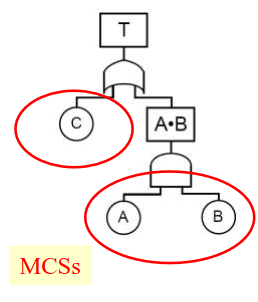
\includegraphics[width=.5\textwidth]{figures/dep-ft-mcs.png}
  \end{center}
  \caption{Esempi di minimal cutset in per il fault tree}\label{fig:mcs-example}
\end{figure}


\paragraph{Fault Tree e algebra di bool}Essendo rappresentati come funzioni logiche, i 
fault tree possono essere semplificati utilizzando le regole dell'algebra di Boole. Ad, 
esempio, l'albero in Figura \ref{fig:dep-ft-ex} genera un espressione del tipo 
\[
  A \lor (B \lor C) \land (C \lor (A \land B))
\]
che può essere semplificata in $C\lor(A\land B)$, rappresentata in Figura 
\ref{fig:dep-ft-sempl}.

\begin{figure}
  \centering
  \begin{subfigure}{0.5\textwidth}
    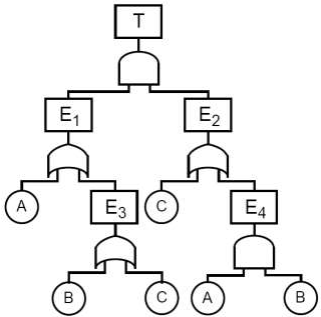
\includegraphics[width=.64\textwidth]{figures/dep-tree-ex.png}
    \caption{Fault tree di partenza}
    \label{fig:dep-ft-ex}
  \end{subfigure}\hfil
  \begin{subfigure}{0.5\textwidth}
    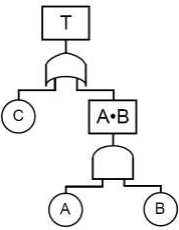
\includegraphics[width=.5\textwidth]{figures/dep-tree-sempl.png}
    \caption{Fault tree semplificato}
    \label{fig:dep-ft-sempl}
  \end{subfigure}
  \caption{\ref{fig:dep-ft-ex}Fault tree di esempio. 
  \ref{fig:dep-ft-sempl} Fault tree dopo la semplificazione con algebra di Bool}
\end{figure}

\paragraph{Da fault tree a RBD e viceversa}Dato un fault tree è possibile passare 
a un RBD e viceversa. Infatti, basta sostituire $AND$ con paralleli e $OR$ con serie 
per passare a RBD e viceversa. In Figura \ref{fig:dep-rbd2ft-1}, è mostrato un semplice 
RBD di un sistema di comunicazione. Analizzandolo si può arrivare alla funzione:
\[
  \overline{\phi} = \overline{c}_1\overline{c}_2 + \overline{v}_1\overline{v}_2\overline{v}_3
\]
che genera il fault tree in Figura \ref{fig:dep-rbd2ft-2}.

\begin{figure}
  \centering
  \begin{subfigure}{0.5\textwidth}
    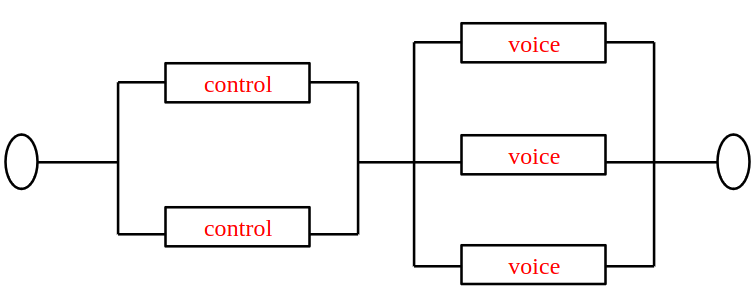
\includegraphics[width=.75\textwidth]{figures/dep-rbd2tree-1.png}
    \caption{RBD di un sistema di comunicazione}
    \label{fig:dep-rbd2ft-1}
  \end{subfigure}\hfil
  \begin{subfigure}{0.5\textwidth}
    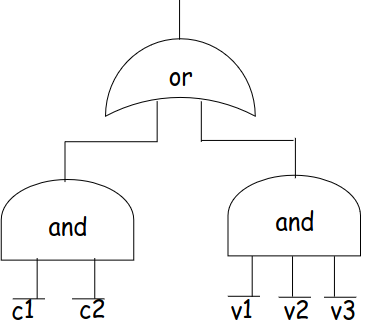
\includegraphics[width=.65\textwidth]{figures/dep-rbd2tree-2.png}
    \caption{Fault tree ricavato dal RBD in Figura \ref{fig:dep-rbd2ft-2}}
    \label{fig:dep-rbd2ft-2}
  \end{subfigure}
  \caption{\ref{fig:dep-rbd2ft-1} RBD di partenza. 
  \ref{fig:dep-rbd2ft-2} Fault tree ricavato}
\end{figure}

La reliability di un fault tree senza eventi ripetuti può essere calcolato attraverso lo 
stesso algoritmo utilizzato per l'RBD. 

\paragraph{Fault tree con eventi ripetuti}Un fault tree con eventi ripetuti non può essere 
trasformato in RBD per il calcolo della reliability, ma è possibile usare uno dei seguenti
approcci:
\begin{itemize}
  \item Factoring algorithm: approccio simile al conditioning in cui si risolve il fault tree 
    assumendo l'evento ripetuto una volta fallito e una volta no. Nell'esempio $\overline{m}_3
    $ è un evento ripetuto. L'analisi con la fattorizzazione produce due altri alberi come 
    in Figura \ref{fig:ft-factoring};
  \item Somma di prodotti disgiunti: si esprime il complemento della funzione uscita 
    dell'albero come somma di prodotti (eventi disgiunti) e si calcola la reliability;
  \item Binary Decision Diagram: non trattati al corso;
\end{itemize}

\begin{figure}
  \begin{center}
    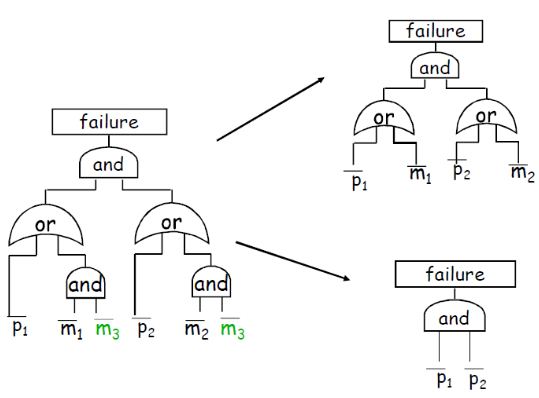
\includegraphics[width=.65\textwidth]{figures/dep-ft-factoring.png}
  \end{center}
  \caption{Esempio di conditioning con fault tree}\label{fig:ft-factoring}
\end{figure}
\clearpage

\subsection{Risk assessment}
L’argomento safety critical ha nel tempo assunto importanza via via più rilevante; la 
necessità di sviluppo di software sicuro in ambito prevalentemente aereospaziale ha portato
alla nascita di diversi standard, con requisiti di sicurezza piuttosto stringenti, al punto 
da far coincidere safety e security. Dunque gli standard citata sono stati ottenuti a seguito
di una serie di direttive della NASA; a causa di diversi fallimenti in diverse missioni
spaziali. Le direttive includevano:

\begin{enumerate}
  \item Nessuna funzione software deve essere lanciata se non strettamente
    necessaria;
  \item Il testing deve essere fatto in maniera completa e con input realistici.
    Qualsiasi tipo di simulazione deve essere completata a tempo di col-
    laudo, prima del lancio della missione;
  \item Per ogni componente software implementato dal sistema è fondamen-
    tale certificarlo
  \item Bisogna identificare e verificare tutte le assunzioni che vengono fatte
    sul codice.
\end{enumerate}

\paragraph{RAMS - Reliability, availability, mantainability e safety} RAMS è una famiglia 
di tecniche utilizzate per gestire i problemi principali del dependable computing. In 
sostanza ci sono divisioni aziendali che studiano i parametri RAM prima ancora di progettare
le soluzioni. La safety, invece, deve essere misurata sul sistema concreto. Lo stesso
dipartimento RAMS si occupa in seguito di certificare il software, e garantire per la sua
affidabilità, applicandosi a tutto il mondo della reliability e della security. 
RAMS coinvolge infatti le attività che mirano a dimostrare attributi, a proteggere minacce
applicando certi mezzi.

\subsubsection{Hazard assesment}
Nell’ambito di sistemi critici, l’analisi dei rischi e dei possibili fallimenti diventa
cruciale, dati i costi molto elevati sia per lo sviluppo, che per i fallimenti stessi. I 
fallimenti in tali sistemi, come già detto, sono catastrofici e devono dunque essere evitati. 
Nell’Hazard Assessment si cerca di evitare situazioni di pericolo potenziale,
dette Hazards, che possono avere un impatto significativo sia per l’ambiente che per la
vita delle persone. Infatti, si ricorda che il rischio è dato dalla probabilità di 
verificarsi di un'hazard per il danno che questo provocherebbe.

Dunque l’identificazione degli hazard è un processo ingegneristico, che
dipende da esperienza e sensibilità di coloro i quali se ne occupano. Tipi-
camente il processo di Hazard Analysis, e quindi della loro identificazione, è
iterativo, e quindi ciclicamente ripetuto ogni volta che il processo di sviluppo
avanza.
Ciò naturalmente implica un aumento dei costi non trascurabili; nella fasi
iniziali il processo è semplice e si cercano di fare analisi a partire dai requi-
siti: si identificano così gli hazards con semplici, seppur intense, sessioni di
\textbf{brainstorming}, e si fa una prima scrematura dei possibili fallimenti.

Esistono varie metodologie da poter applicare: una molto usata è quella
della HAZOP, Hazard and operability Study, così come anche la Failure
Modes and Effect Analysys, FMEA, che vedremo a breve. Anchi i fault
trees, già descritti nella sezione precedente, vengono usati. Non disdegnamo
inoltre la metodologia What if, molto in linea con il pensiero umano, che
consiste nell’immaginare scenari eventuali in risposta ad un certo fallimento. 

Data una lista di hazard dalla fase di brainstorming si rende necessario
sfoltirla e selezionare solo quelli più pertinenti, per passare poi ad una for-
malizzazione degli harzard stessi. Dato per esempio il sistema automobile,
e dati i ragionamenti, l’obiettivo è dare una formalizzazione vera e propria,
identificando cause e conseguenze.
Tale scrematura è quindi fatta convertendo gli Hazard in Rischi, dove ri-
cordiamo il rischio è la severità del fallimento per l’occorrenza el fallimento
stesso. Per intenderci, se uno tsunami colpisse il nostro meraviglioso cottage
in montagna, questo verrebbe certamente disintegrato. è però anche vero
che la possibilità che uno tsunami colpisca il cottage sia anche estremamente
improbabile, ergo il rischio è nullo.

\subsubsection{FMEA - Failure Mode and Effect Analysis}
La Failure Modes and Effect Analysis, è una tecnica di Hazard Analysis di tipo bottom up,
che parte dall’analizzare i componenti nel sistema e poi capire come dal fallimento dei 
singoli componenti si possa giungere al fallimento di altri componenti a cascata,e al 
fallimento dell’intero sistema.

Gli obiettivi che ci si pone sono l’identificazione delle possibili cause di fallimento di
un sistema, i potenziali effetti sull’esecuzione del sistema e poi naturalmente mezzi di
mitigazione ed eventuali azioni correttive. Tutte queste fasi, in principio sequenziali, 
sono anche cicliche, e applicate ogni qualvolta si rende necessaria la gestione di rischi
nel sistema. Di seguito i passi fondamentali per tale analisi, che prendono il nome di
\textbf{Risk Management}:

\begin{enumerate}
  \item dentificazione dei componenti, con le loro funzionalità e i loro possibili
    fallimenti, detti anche modi di fallimento;
  \item per ogni modo di fallimento identificato bisogna capire gli effetti che tale
    modo ha sull’intero sistema. Se pe esempio si rompesse un sensore in un
    sistema di rilevamento frane consistente in soli 2 sensori, il fallimento di
    uno di questi sarebbe critico, e comporterebbe il fallimento dell’intero
    sistema. Viceversa se i sensori fossero a decine, il fallimento di uno
    potrebbe non avere grande rilievo; ma ciò dipende naturalmente dal
    tipo di fallimento; 
  \item Una volta raccolti tali modi, è necessario stabilire la severity, ovvero
    quale è il costo sopportato in caso di fallimento. Tale parametro è
    calcolabile in base agli effetti del fallimento. Si cerca poi di capire le
    cause di tale fallimento e poi la probabilità che questo occorra. 
  \item ovviamente tutti i fallimenti potrebbero non esser rilevati. Dunque
    il rischio deve esser calcolato tenendo conto anceh del parametro di
    identificazione, o Detection che rappresenti l’abilità di individuare
    potenziali cause $Risk = Severity\, x\, Occurrence\, x\, Detection$ 
  \item Stabiliti questi parametri è possibile determinare il rischio secondo la
    formula vista in precedenza
  \item ordinando i rischi in ordine, dal maggiore al minore, otteniamo un ranking dei rischi,
    e quindi possiamo stabilire su quali rischi concentrarci
    e su quali proporre tecniche di mitigazione o di correzione del design. Il processo viene
    quindi rieseguito dal punto 1 finchè non sono stati controllati tutti i componenti.
\end{enumerate}

L’analisi FMEA (Figura \ref{fig:fmea}) prevede una estensione che tenga conto solo di hazard
con effetti critici, chiamata FMECA. Definiti cause ed effetti si può stabilire se il
componente di un fallimento sia critico per l’intero sistema o meno. Il fallimento di tal
componente può avere effetto su di un altro componente, e, in caso affermativo, si devono
fare tutti gli step citati in precedenza, altrimenti si può tornare alla fase di 
ripetizione finchè tutti i componenti non sono stati analizzati,sempre in accordo con la
dicitura precedente.

\begin{figure}
  \begin{center}
    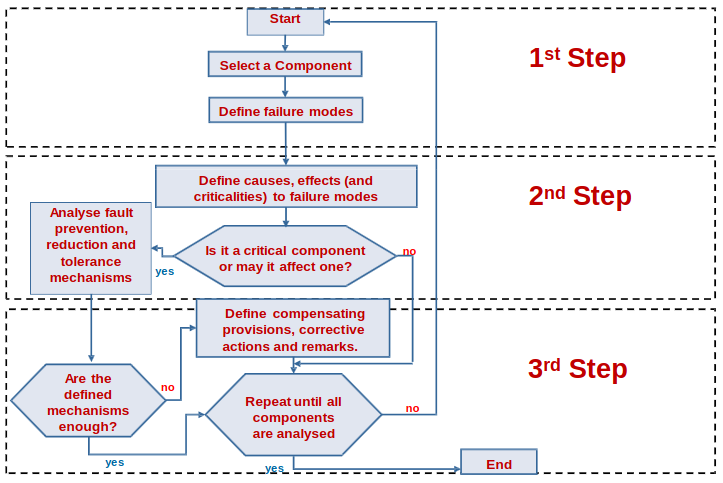
\includegraphics[width=.7\textwidth]{figures/dep-fmea.png}
  \end{center}
  \caption{Processo FMEA}\label{fig:fmea}
\end{figure}

Nella identificazione di un failure mode ci chiediamo come un componente possa fallire, 
quindi come esso possa deviare rispetto alle proprie specifiche. Per ogni sottocomponente
del sistema, si stabiliscono i potenziali modi di fallimento, come lo stuck at zero, il
null reading, lo stuck at N, eventuali reset, isolamento dei sensori e via dicendo. Questi
possono essere presi tipicamente dai datasheet dei sensori per esempio, oppure da interventi di
manutenzione. Gli effetti li si ottengono costruendo un effect tree analysis : di tutti gli
effetti si costruisce un albero così da capire gli effetti di propagazione. Una volta 
ottenuti suddetti effetti, si realizza un rank. Possiamo stimare ffetti pericolosi senza
avvisaglie, con un massimo valore di 10, fino a ad effetti nulli al livello 1, passando per
effetti medio/alti con valore 6, dove il sistema diventa non operativo e l’equipaggiamento
a sua disposizione risulta danneggiato. 

Per l’occorrenza si cerca, per ogni effetto, la percentuale di avventimento di un 
fallimento tramite questionari, brainstorming e secondo analisi dell’ambiente sul quale 
operare. E anche qui si stabilisce un ranking da 1 a 10. Un ranking 10 coincide con 
probabilità di fallimento pari al 50\% o più, 6 sarà fallimento occasionale con 1 
fallimento ogni 80 circa, fino al ranking 1 con fallimento remoto. Analogamente si 
effettuano le stesse analisi la detection.

Infine, un procedimento viene fatto anche per la detection. Infatti, Figura 
\ref{fig:dep-detection-ranking} è mostrato un ranking per la detection.

\begin{figure}
  \begin{center}
    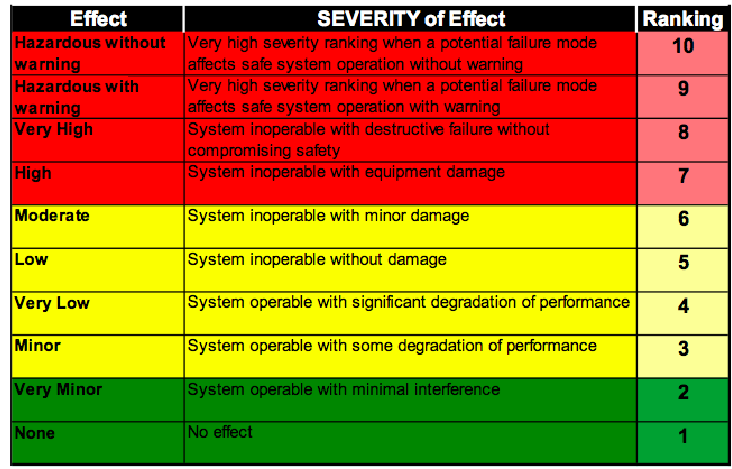
\includegraphics[width=.6\textwidth]{figures/dep-effect-ranking.png}
  \end{center}
  \caption{Tabella prodotta dall'analisi degli effetti}
\end{figure}

\begin{figure}
  \begin{center}
    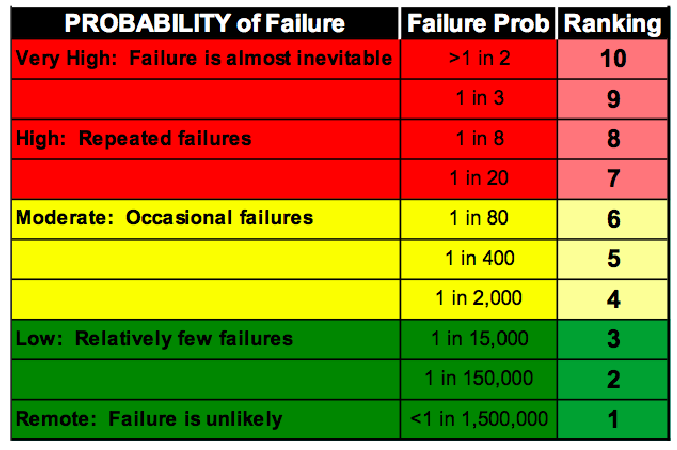
\includegraphics[width=.6\textwidth]{figures/dep-occurrence-ranking.png}
  \end{center}
  \caption{Tabella prodotta dall'analisi delle occorrenze}
\end{figure}

\begin{figure}
  \begin{center}
    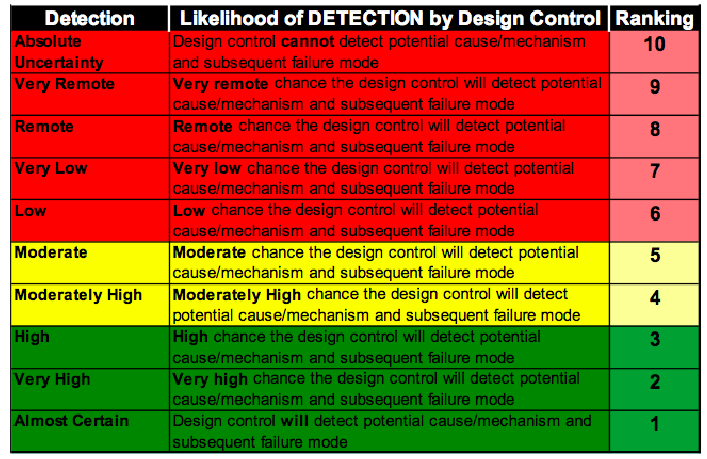
\includegraphics[width=.6\textwidth]{figures/dep-detection-ranking.png}
  \end{center}
  \caption{Tabella prodotta dall'analisdella detectionn}\label{fig:dep-detection-ranking}
\end{figure}

\subsubsection{Software fault tolerance}
Le buone pratiche dell’ingegneria del software prevedono anche alcune tecniche relative 
alla gestione di guasti, come ad esempio quelle di \textbf{Fault avoidance} e 
\textbf{Fault tolerance}. Nel primo caso si cerca di realizzare un software sicuro, in modo
da minimizzare le probabilità di fallimento. Tuttavia dimostrare che un modulo software sia
privo di errori non è possibile, in quanto il testing del software può solo mostrare la
presenza di eventuali bug, ma non la loro assenza, secondo riportato dalla tesi di Dijkstra.

Poichè non è possibile ridurre a zero la probabilità di fallimento, l’approccio del 
Fault Tolerance preveda che un sistema software mantenga un comportamento corretto, aderente
alle specifiche, anche in presenza di stati alterati.
L’insieme delle metodologie, tecniche e tecnologie atte a evitare l’introduzione di guasti 
nel design prende invece il nome di Fault Prevention, mentre l’insieme di tecniche 
utilizzate per eliminare guasti dal software, viene identificata con nome di Fault Removal, 
che si articola solitamente in fasi di verifica, analisi e testing.

Le tecniche di tolleranze ai guasti software sono di 2 tipi:
\begin{itemize}
  \item \textbf{Single Version}: le più economiche e che non richiedono di
    implementare differenti varianti e cercano in qualche modo di aggiungere meccanismi per
    rilevare il guasto, contenerlo e correggerlo.
  \item \textbf{Multi version}: usano varianti differenti del modulo software. Esse sono però 
    soluzioni molto costose, poich´e partendo dai requisiti devono implementare più varianti 
    di uno stesso modulo software, garantendo fallimenti indipendenti.

\end{itemize}
\paragraph{Single Version Fault Tolerance -  Robust data structure} Le strutture dati 
possono essere rese più robuste al fine di rilevare degli errori o addirittura di
correggerli, inserendo ridondanza a livello di dati. Per esempio una lista a puntatori, 
possiede, come ben noto, nodi con puntatori al nodo successivo, mentre il nodo finale 
possiede un puntatore a NULL. Se dovesse accadere un errore in uno dei puntatori next dei
nodi, non ci sarebbe modo ne di rilevarlo ne di correggerlo. 

Tale lista può esser però resa circolare, facendo puntare l’ultimo elemento alla testa
e non a NULL. Cos`ı un errore in un puntatore potrebbe essere quantomeno rilevato perch´e
non sarebbe più possibile completare il ”giro” della lista, tornando alla testa, perchè
uno dei puntatori romperebbe la catena. Ciò significa identificare l’occorrenza dell’errore,ù
ma non poterlo correggere. Se si vuole correggere l’errore è necessario usare una lista
doppiamente linkata, mantenendo la circolarità; con questo tipo di struttura si possono
identificare fino a 2 errori sui puntatori, ma non correggerli entrambi. La struttura si dice
2 detectable e 1 correctable, perchè almeno uno degli errori è corregibile. Una volta 
rilevato l’errore, si utilizza infatti il senso opposto di percorrenza, e quindi il suo
ordinamento per poter correggere il puntatore sfasato. Circa invece errori sulla consistenza
dei dati è possibile aggiugnere ridondanza all’interno dei nodi. 

\paragraph{Single Version Fault Tolerance -  Checkpointing and Restart} Questa tecnica 
(Figura \ref{fig:checkpoint-and-restart}) parte dall’assunzione che gli errori e i fallimenti
che si manifestano durante l’esercizio di un sistema sono difficilmente riproducibili e hanno
una caratteristica di transitorietà. Il checkpoint consiste nel salvare tutto lo stato
d’esecuzione del modulo software,dopodichè, durante l’esecuzione, in caso di errore, verrebbe
innescata un azione di ripristino, consistente nel reset del sistema e nel caricamento dello
stato d’esecuzione salvato nella fase di checkpoint.

\begin{figure}
  \begin{center}
    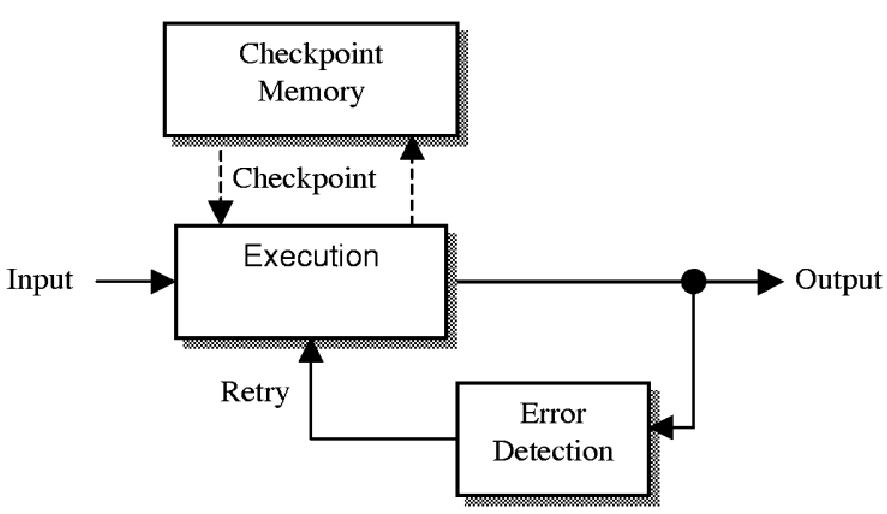
\includegraphics[width=.5\textwidth]{figures/dep-sw-checkpointing.png}
  \end{center}
  \caption{Schema della tecnica del checkpointing}\label{fig:checkpoint-and-restart}
\end{figure}

Una variante più complessa di questo modello è quella del \textbf{Process Pair} (Figura
\ref{fig:checkpoint-process-pair}). In questo caso, si fa sempre uso del checkpoint e si
cerca di diminuire l'MTTR. Ad esempio, quando si installa un aggiornamento sul SO, se 
questo non va a buon fine, il ripristino del sistema può essere lento nel caso visto in 
precedenza. Per ovviare a ciò, e diminuire il tempo medio per il recovery, si utilizzano
due nodi, con due sistemi operativi e due copie del modulo software. Viene così fatto il
checkpoint del modulo primario e viene traserito al sistema di backup Quando viene rilevato
un errore, l’elemento primario si isola dal sistema, e viene eletto il backup come nuovo
modulo primario, consistente con l’ultimo checkpoint, che permette di continuare
l’esecuzione dell’aggiornamento a costo pari a quello del cambio di contesto.

\begin{figure}
  \begin{center}
    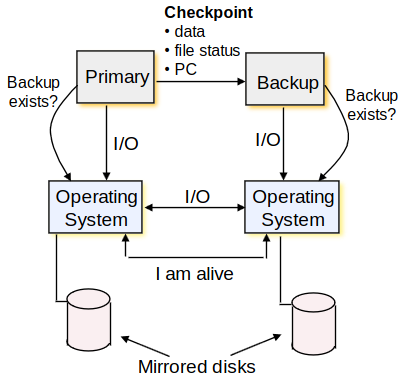
\includegraphics[width=.5\textwidth]{figures/dep-sw-processpair.png}
  \end{center}
  \caption{Tecnica del process pair}\label{fig:checkpoint-process-pair}
\end{figure}

\paragraph{Multi Version Fault Tolerance - N-versioning}Nel modello N-versioning (Figura 
\ref{fig:nversioning}) si riduce la dipendenza dai fallimenti e si aumenta la
probabilità che i fallimenti siano tra loro indipendenti. Adottare più varianti cerca
di affrontare problemi di guasti che non sono necessariamente transitori, e che possono
dunque rendere difficile gestioni basate su checkpoint. È chiaro ovviamente realizzare
differenti versioni del sistema implica un aumento considerevole di costi.

Lo stesso input è quindi imposto ad ogni singola variante, usando canali software distinti
per mantenere quanto più possibile indipendenzasarà poi un algoritmo di decisione a 
stabilire quale sarà l’output da fornire. Ciò si traduce nell’implementazione di un TMR a
livello software software, minimizzando i fallimenti di modo comune.

\begin{figure}
  \begin{center}
    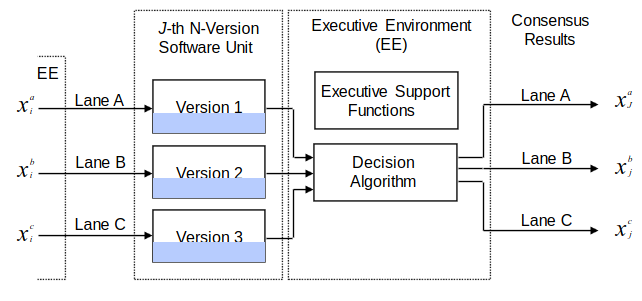
\includegraphics[width=0.6\textwidth]{figures/dep-sw-nversioning.png}
  \end{center}
  \caption{Schema di funzionamento dell'$n$-versioning}\label{fig:nversioning}
\end{figure}

Nonostante venga usato nella maggior parte dei sistemi critici moderni, l’approccio 
Multi Version non fornisce alcuna stima quantitativa su quanto si riduca la probabilità che i moduli 
falliscano in maniera dipendente. Si sta lavorando però su come predire in maniera quantitativa
tale valore.
Il problema grande del N-version programming è fondamentalmente nei requisiti. Se vogliamo
far sviluppare due versioni dello stesso modulo software, dobbiamo esser sicuri che i
requisiti siano corretti e concreti, effettuando verifiche su correttezza e completezza,
evitando la presenza requisiti ambigui.

Nella pratica si usano due versioni del modello ad N-versioning:
\begin{itemize}
  \item \textbf{N-self checking programming}: dove ogni versione ha un proprio acceptance
    test, ed una successiva logica di decisione prende l’uscita del componente in
    accoppiamento con quella fornita dall’acceptance test, per fornire poi l’output adatto
    (Figura \ref{fig:nversioning-self});
  \item \textbf{N-self checking programming using comparison}: prevede di fare una 
    comparazione per rilevare errori, versione per versione, che vengono comparate a coppie
    per decidere poi l’output corretto. Come configurare i comparatori è difficile da
    decidere, perch´e stabilire se ci sia un errore o meno dipende dal tipo di 
    applicazione (Figura \ref{fig:nversioning-self-comp});
\end{itemize}

\begin{figure}
  \begin{center}
    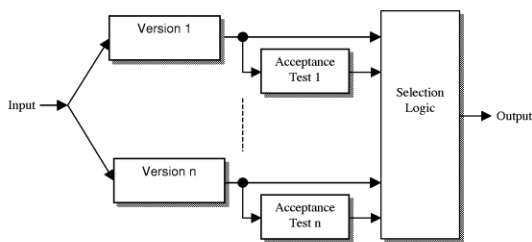
\includegraphics[width=0.5\textwidth]{figures/dep-sw-nversioning-self.png}
  \end{center}
  \caption{Schema di funzionamento dell'$n$-self checking programming}
  \label{fig:nversioning-self}
\end{figure}

\begin{figure}
  \begin{center}
    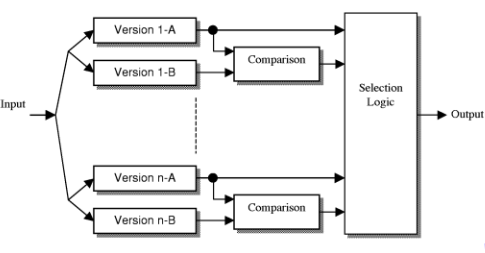
\includegraphics[width=0.5\textwidth]{figures/dep-sw-nversioning-self-comp.png}
  \end{center}
  \caption{Schema di funzionamento dell'$n$-self checking programming con comparazione}
  \label{fig:nversioning-self-comp}
\end{figure}

\clearpage
\subsection{FFDA - Field failure data analysis}
Quando è stata introdotta l'analisi 
delle performance, in Figura \ref{fig:metric_overview} si è evidenziato che studi come il 
capacity test vanno effettuati solo quando il sistema non presenta errori, mentre altre 
analisi si effettuano per caratterizzare come questo fallisce. La 
\textbf{\textit{field failure data analysis (FFDA)}} è una tecnica per la stima degli 
attributi di dependability basata su misure dirette. 

I processi che utilizzano misure dirette sono i più costosi e impegnativi poichè richiedono
una comprensione profonda del sistema in esame, ma sono anche quelli che forniscono risultati 
più vicini alla realtà. L'FFDA si propone di raggiungere i seguenti obiettivi:

\begin{enumerate}
  \item identificazione e classificazione di errori e fallimenti, così come si manifestano 
    sul campo, con la loro severità e la loro correlazione. dunque la FFDA è utile per 
    derivare modelli di fallimento;
  \item Studio delle distribuzioni statistiche di tempi di fallimento e recovery;
  \item Analisi di correlazione tra i fallimenti e il workload, fondamentale soprattutto
    per sistemi critici;
  \item Modellazione del comportamento di fallimenti e di eventuali meccanismi di recovery;
  \item dentificazione delle cause di fallimenti e di \textit{bottleneck};
  \item validazione e popolazione di modelli di fallimento simulativi. L’RBD, così come
    visto, è un modello combinatorio e rappresenta il sistema tramite componenti 
    indipendenti con fallimenti indipendenti. I valori di reliability proposti dal modello 
    però, oltre a poter essere teorici, possono anche esser messi a disposizione dal 
    fornitore, il quale li avrà ottenuti tramite un monitoraggio del sistema e misure 
    dirette.
\end{enumerate}

Come tutte le altre tecniche su misure dirette, la FFDA studia solamente i fallimenti che si 
manifestano, ma alcuni come detto in precedenza possono essere mascherati. Inoltre, tutti i 
dati raccolti e le conclusioni raggiunte con uno studio sono fortemente dipendenti dall'
\textbf{ambiente} in cui questo opera e difficilmente generalizzabili. Per questo motivo, 
gli studi dovrebbero essere eseguiti su diversi sistemi, che operano su ambienti diversi 
con lunghi periodi di osservazione.

\paragraph{Metodologia della FFDA}La FFDA parte da dati grezzi (\textbf{\textit{raw data}}) 
e arriva a presentare dei risultati tangibili attraverso un processo (Figura
\ref{fig:ffda-process}) ben definito che parte con l'acquisizione dei dati
(\textbf{\textit{data logging & collection}}). Segue la fase di filtraggio
(\textbf{\textit{filtering}}) che si occupa di eliminare le informazioni non interessanti.
La parte cruciale della FFDA è quella con cui si cerca di correlare tra loro gli errori per
identificare un singolo fallimento del sistema (\textbf{\textit{data manipulation}}). 
Infine, si possono analizzare i dati ottenuti cercando di caratterizzare i dati 
attraverso \textbf{\textit{fitting}} con una distribuzione nota.

\begin{figure}
  \begin{center}
    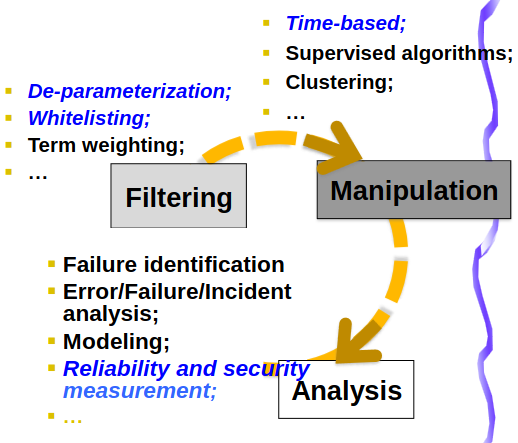
\includegraphics[width=.5\textwidth]{figures/dep-ffda.png}
  \end{center}
  \caption{Processo FFDA}\label{fig:ffda-process}
\end{figure}

Nei paragrafi che seguono vengono date più indicazioni sulle singole fasi.

\subsubsection{Data collection and logging}
La fase di \textbf{\textit{data logging e collection}} consiste nel definire cosa raccogliere
e come. Le principali tecniche sono quella della \textbf{failure reports} e \textbf{event
logs}.

\paragraph{Failure reports} I fallimenti di sistemi sono rilevati tramite dei report, 
ovvero dei documenti compilati in maniera semiautomatica, come accade ad esempio in Windows,
e validati da un operatore umano. Ogni report è solitamente caratterizzato da un timestamp 
, una descrizione di quello che si è osservato, una supposizione della causa, sia essa 
hardware o software, ed eventualmente i tentativi di ripristino effettuati. 
Il vantaggio dei report, e che non è necessario effettuare analisi ampie dei dat il, in 
quanto la garanzia di un operatore viene considerata sufficiente. Questa è però un’arma a
doppio taglio, in quanto i failure sono identificati dagli umani, e quindi al crescere del
sistema si è proni al non identificare tutti i fallimenti, oltre che essere dipendenti
dalla soggettività degli operatori umani.

\paragraph{Event logs}I log vengono generati direttamente dalla macchina, come accade in
sistemi operativi come Unix. I log sono compostoi da un timestamp, una descrizione dell’
evento, una sorgente (un processo solitamente) e dal tipo di evento. Il problema dei log è
che solitamente il numero di task in esecuzione su di un sistema operativo può essere 
abbastanza alto, e un fallimento viene riportato da ogni task che identifica tale
fallimento. Ciò si traduce nell’avere diverse entry nel Log relative ad un unico problema.

\subsubsection{Filtraggio}Il filtraggio ha la funzione di rimuovere i dati inutili 
da quelli originali ottenendo un dataset più piccolo e più gestibile. Esistono due strategie:
\begin{itemize}
  \item \textbf{White listing}: vengono inclusi nel dataset di uscita tutte le entry che 
    hanno un riscontro con un pattern di interesse. Ad esempio, si può specificare di 
    essere interessati a tutti gli errori che riguardano la rete o CPU;
  \item \textbf{Black listing}: tutti gli eventi che hanno riscontro con un determinato 
    pattern \textbf{non} vengono inclusi nel dataset di uscita.
\end{itemize}

\paragraph{De-parametrizzazione}La deparametrizzazione consiste nell'analizzare la struttura 
di un entry del log per capirne quali sono le parti invarianti e quali invece possono essere 
rimpiazzate con \textbf{token} per ottenere dei pattern. I pattern possono essere utilizzati
per effettuare \textbf{\textit{query}} più avanzate sul dataset utili per la fasi
successive. In Figura \ref{fig:deparametrization-1}, è mostrato un file di log da analizzare. 
Osservando le parti in rosso, si nota che ogni entry del file può essere sostituita come 
in Figura \ref{fig:deparametrization-2}.

\begin{figure}
  \centering
  \begin{subfigure}{0.5\textwidth}
    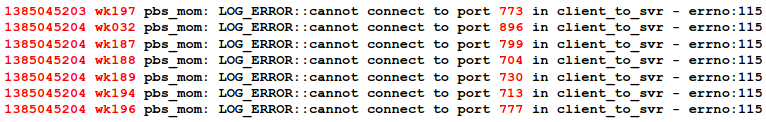
\includegraphics[width=0.95\textwidth]{figures/dep-deparametrization1.png}
    \caption{File di log non deparametrizzato}
    \label{fig:deparametrization-1}
  \end{subfigure}\hfil
  \begin{subfigure}{0.5\textwidth}
    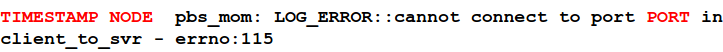
\includegraphics[width=0.95\textwidth]{figures/dep-deparametrization2.png}
    \caption{Entry de-parametrizzata}
    \label{fig:deparametrization-2}
  \end{subfigure}
\end{figure}

L'obiettivo della de-parametrizzazione è quello di creare un \textbf{dizionario} con dei
pattern di dimensioni ridotte. Un dizionario è facilmente analizzabile da esperti di dominio
in quanto di solito è composto da poche centinaia di righe (rispetto a un file di log che 
può contenere milioni di entry) e quindi può essere utilizzato per produrre \textit{white- 
list} mirate per estrarre informazioni su eventi di interesse. Il processo è riassunto in 
Figura \ref{fig:dictionary}.

\begin{figure}
  \begin{center}
    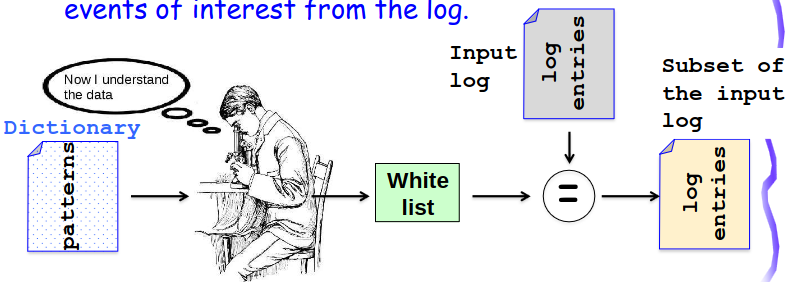
\includegraphics[width=.6\textwidth]{figures/dep-dictionary.png}
  \end{center}
  \caption{Utilizzo di un dizionario per ridurre il log iniziale}\label{fig:dictionary}
\end{figure}

\subsubsection{Manipolazione dei dati}
La ricerca ha spinto molto per lo sviluppo di tecniche innovative basata sull'intelligenza
artificiale. Tuttavia, risultati accettabili si ottengono ancora oggi con \textbf{metodi
basati sulla coalescenza}. Questi metodi raggruppano le entry di un file di log cercando 
correlazioni tra i dati. Queste correlazioni possono essere di carattere \textbf{temporale}
(se si raggruppano i dati su una finestra temporale), \textbf{spaziale} (se si raggruppano i 
dati in base a tipi di nodi diversi; utile in sistemi distribuiti), \textbf{sul contenuto} 
(se le entry vengono raggruppate per tipologia di errori etc\dots).

L'obiettivo della coalescenza è produrre una \textbf{tupla}: una lista di entry del log 
iniziale relative allo stesso fallimento. Idealmente, ad ogni tupla corrisponde un 
fallimento. 


\paragraph{Coalescenza temporale}L'analisi vista al corso si basa sulla coalescenza temporale. 
Detta $W$ la dimensione di una finestra temporale (\textbf{\textit{window size}}), le tuple
vengono semplicemente create con l'algoritmo in Listato \ref{alg:temp-coalescence}.
\begin{algorithm}
  \begin{algorithmic}
    \If{$t(X_{i+1}) - t(X_i) < W$}
    \State Add $X_{i+1}$ alla tupla
    \EndIf
  \end{algorithmic}
  \caption{Algoritmo per la coalescenza temporale}
  \label{alg:temp-coalescence}
\end{algorithm}

Usare la corretta $W$ è cruciale. Una $W$ troppo grande genera una \textbf{collisione}: nella
stessa tupla possono cadere più fallimenti separati. Invece,una $W$ troppo piccola genera un
\textbf{troncamento}: lo stesso fallimento si trova in più tuple differenti.

Una pratica comune è quella di tentare diversi valori di window size e rappresentare il numero 
di tuple ottenute su un grafico. Il punto di \textit{knee} del grafico ottenuto può essere 
una buona approssimazione per la $W$. In Figura \ref{fig:cwin}, è mostrato un esempio 
di grafico per la stima della $W$: il punto di knee indica che il valore ottimale è $W=240$ 
con $276$ tuple.

\begin{figure}
  \begin{center}
    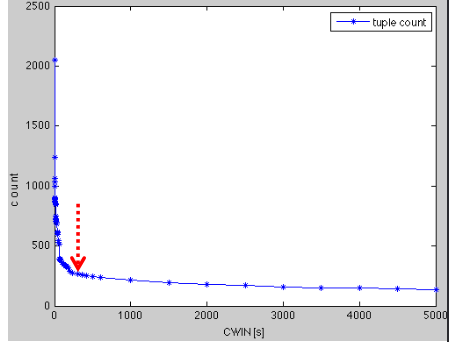
\includegraphics[width=.5\textwidth]{figures/dep-cwin.png}
  \end{center}
  \caption{Esempio: numero di tuple per dimensione della window size}\label{fig:cwin}
\end{figure}

\subsubsection{Analisi dei dati}
Bisogna effettuare un'analisi sui dati manipolati per identificare trend. Di solito, si
svolgono analisi sui tempi di fallimento e classificazione di questi (si è interessati alla 
natura dei fallimenti: transitorio, permanente, intermittente). Infine si cercano di 
stimare MTTF e MTTR. In base al fitting con particolari tipi di distribuzione si possono fare 
assunzioni sul tipo di guasto. 

\paragraph{Distribuzione esponenziale}Tipo di distribuzione più semplice: può essere usata
per modellare guasti indipendenti (tipicamente di natura elettronica) con un failure rate 
$\lambda$ costante. In Figura \ref{fig:pdf-exp}, è mostrato l'andamento di una pdf 
esponenziale, contraddistinta dalle funzioni in Tabella \ref{tab:exp-pdf}.

\begin{table}
  \begin{center}
    \begin{tabular}[c]{l|l}
      \hline
      \multicolumn{1}{c|}{\textbf{Funzione}} & 
      \multicolumn{1}{c}{\textbf{Espressione}} \\
      \hline
      pdf & $f(t) = \lambda e^{-\lambda t}$ \\
      Reliability & $R(t) = 1 - e^{-\lambda t}$ \\
      Failure rate & $h(t) = \lambda$ \\

      \hline
    \end{tabular}
    \caption{Funzioni caratterstiche distribuzione esponenziale}\label{tab:exp-pdf}
  \end{center}
\end{table}

Sebbene sia semplice, questo tipo di distribuzione trova poca applicazione in dati reali
in quanto i guasti sono raramente indipendenti tra loro, ma spesso sono dovuti a cause 
comuni.

\paragraph{Distribuzione lognormale}Questo tipo di distribuzione modella molto bene il 
tasso di fallimenti software. I fallimenti di tipo software sono complessi e dovuti a 
molte cause. L'andamento lognormale viene fuori quando il valore di una variabile è
condizionato da molti fattori randomici.

\begin{figure}
  \begin{center}
    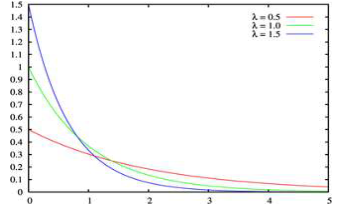
\includegraphics[width=.5\textwidth]{figures/dep-exp-pdf.png}
  \end{center}
  \caption{Esempio: $pdf$ esponenziale al variare di $\lambda$}\label{fig:pdf-exp}
\end{figure}

La funzione di probabilità di una lognormale (Figura \ref{fig:lognormal}) è:
\[
  f(t) = \frac{1}{t\sigma\sqrt{2\pi}}e^{-\frac{(\log t -\mu)^2}{2\sigma^2}}
\]

\begin{figure}
  \begin{center}
    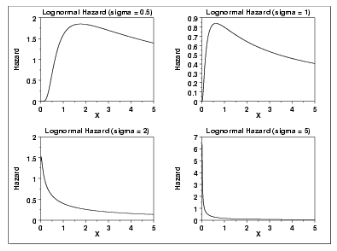
\includegraphics[width=.5\textwidth]{figures/dep-lognormal.png}
  \end{center}
  \caption{Esempio: andamento lognormale}\label{fig:lognormal}
\end{figure}

\paragraph{Distribuzione Weibull}Si tratta di una versione più usata di quella esponenziale 
per modellare tassi di fallimento di compoinenti elettroniche. Attraverso il parametro
$\gamma$ è possibile modellare tutte le fasi della \textit{bath-tube curve}. Le sue
caratteristiche sono mostrate in Tabella \ref{tab:weibull}.

\begin{table}
  \begin{center}
    \begin{tabular}[c]{l|l}
      \hline
      \multicolumn{1}{c|}{\textbf{Funzione}} & 
      \multicolumn{1}{c}{\textbf{Espressione}} \\
      \hline
      pdf & $f(t) = \gamma\lambda t^{\gamma-1} e^{-\lambda t^\gamma}$ \\
      Reliability & $R(t) = 1 - e^{-\lambda t^\gamma}$ \\
      Failure rate & $h(t) = \lambda\gamma t^{\gamma-1}$ \\

      \hline
    \end{tabular}
    \caption{Funzioni caratterstiche distribuzione esponenziale}\label{tab:weibull}
  \end{center}
\end{table}

\subsubsection{Case study: Bluetooth Stack}
Da un punto di vista storico, l’importanza degli studi di FFDA su sistemi di calcolo trova 
spazio già a partire dagli anni 80, dove i sistemi target erano solitamente applicazioni e
sistemi operativi, e gli obiettivi erano relativi all’identificazione di relazioni tra 
fallimenti e carichi sottoposti al sistema. Già negli anni 90 si estese l’interesse di tale 
branca anche a infrastrutture di rete, fino ad arrivare agli anni 2000, comprendendo anche
sistemi su larga scala, macchine virtuale e sistemi embedded e mobile. 

Per esempio tra il 1982 e il 1986 molti studi furono fatti relativamente al rapporto tra
fallimenti e carico; si notò infatti la forte correlazione tra fallimenti e carico, in
quanto la probabilità di un fallimento cresceva all’incrementare di un carico interattivo. 

Il problema principale consisteva nell’emulazione del protocollo IP su Bluetooth, tramite 
un apposito stack, beneficiando dei vantaggi del bluetooth. I nostri eroi necessitavano di
fare una anlisi di tale sistema, al fine di migliorarne le prestazioni in termini di
fallimenti, la cui frequenza era tale da rendere il sistema particolarmente lento.

\begin{figure}
  \begin{center}
    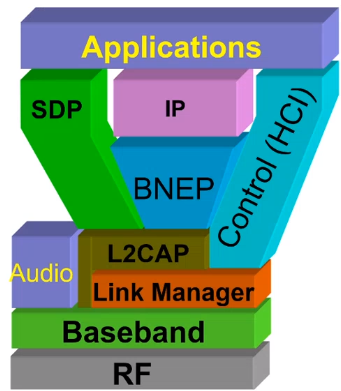
\includegraphics[width=.2\textwidth]{figures/dep-bl-stack.png}
  \end{center}
  \caption{Schema dello stack bluetooth}
\end{figure}

Lo stack bluetooth si basa su di un livello di Baseband dedito alla comunicazione, al time
division multiplexing e al controllo di integrità e ritrasmissione. Il livello 
immediatamente superiore, ovvero il link manager è volto alla creazione di canali data link
e allo scanning, finalizzato all’identificazione dei dispositivi in ascolto, e ai servizi
coperti nell’area di competenza del segnale. Vi era poi uno strato di L2CAP ,che poggiava sul
link manager, e rappresentava una parte del livello ethernet, che si occupava dunque di
segmentazione, assemblaggio e multiplexing dei pacchetti. C’era poi un livello BNEP che emulava de facto ethernet,
così da fare da base d’appoggio per il protocollo IP vero e proprio. Il livello SDP era
usato, come dice l’acronimo, come service discovery protocol, ed era infine presente un
livello di Controllo, oltre che un livello indipendente di gestione audio. 

Il sistema complessivo è stato quindi dispiegato sui client, sullo sniffer e sul server,
dove i client erano in comunicazione tra loro. Ogni client era delegato alla raccolta di
TestLog e SystemLog, lo Sniffer si occupava di raccogliere Log di rete e infine il server
bluetooth si occupava di raccogliere solo log di sistema. Il tutto era infine mandato in
pasto ad un Log Server. 

\begin{figure}
  \begin{center}
    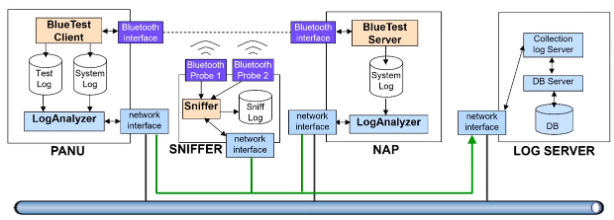
\includegraphics[width=.5\textwidth]{figures/dep-bl-monitor.png}
  \end{center}
  \caption{Schema di monitoraggio del sistema bluetooth}
\end{figure}

A valle di ciò fu effettuato un merging, o unione, tra il test log e il system log, generati
dai componenti del sistema. Questa operazione si traduce banalmente nell’ammassare tutte le 
entry di tali log, per poi ordinarle temporalmente in base al loro timestamp. L’operazione
immediatamente successiva è quella del Tupling, realizzata tramite un algoritmo di 
coalescenza temporale, per accorpare entry relative ad uno stesso errore, quantomeno 
secondo un criterio di vicinanza temporale.

Per intenderci, se dentro una tupla c’era ad esempio un packet loss, e un L2CAP error,
questo fenomeno era dovuto proprio all’errore L2CAP. ovvero se nella stessa tupla si
presentavano entry di log prodotti da diversi componenti, si poteva stabilire una relazione
di propagazione dell’errore.

A questo punto, studiando la frequenza di tuple con questi due errori, possiamo vedere
quale percentuale di packet loss sia dovuta alla L2CAP error, oppure quale errore dipenda
da altri, o a sua volta si propaghi verso altri tipi di fallimento. è possibile quindi,
a partire dal log, estrarne una sorta di catena di Markov, nella quale ogni collegamento
rappresenta naturalmente la probabilità che da un fallimento se ne giunga ad un altro. Il
come queste percentuali vengano estratte, dipende ovviamente dai log, secondo un approccio
frequentistico.

\begin{figure}
  \begin{center}
    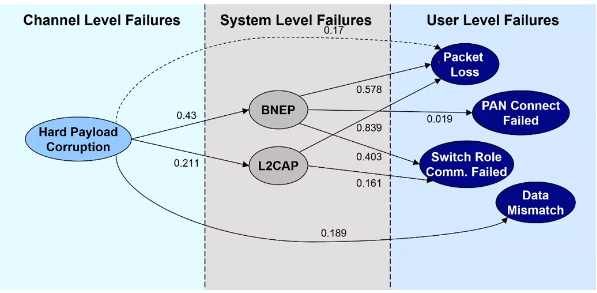
\includegraphics[width=.5\textwidth]{figures/dep-bl-markov.png}
  \end{center}
  \caption{Modello markoviano per l'errore di tipo \textit{Hard payload corruption}}
  \label{fig:markov-bt}
\end{figure}
In Figura \ref{fig:markov-bt},si nota come un errore di Hard Payload Corruption a livello
canale, al 43\% può causare un errore L2CAP a livello sistema, che può causare, nell’83\%
dei casi, un errore di perdita di pacchetti.

Si notò che La bind della socket falliva a causa di una sincronizzazione non corretta, 
ovvero una race condition, con una frequenza elevatissima. Dunque quando L’operazione di Bind
veniva richiamata, doveva essere già presente una connessione bluetooth. Il tempo necessario
a creare la connessione era $T_c$, mentre $T_H$ era il tempo di configurazione per 
l’interfaccia BNEP. Se la richiesta di binding avveniva entro queste due finestre temporali,
ovvero prima che la connessione bluetooth di fatto esistesse, il binding falliva, restituendo
errori diversi in base all’intervallo temporale in cui ricadeva la richiesta. 

La soluzione stava nel richiamare il binding al di fuori di tali intervalli, modificando lo
stack protocollare tramite una magica sleep di durata $T_c +T_H$.

Altra cosa interessante che fu realizzata furono le Software recovery actions: per ogni
fallimento rimanente, si provarono diverse di queste azioni di recovery, dette SIRA
partendo dal riavvio di servizi a severity di fallimento minore, arrivando fino a reboot
dell’intero sistema. Si notò così che facendo uno stack reset, si risolveva il problema
nel 61\% dei casi, e così per diversi altri errori.

\clearpage
\subsection{Sicurezza}
Con il termine \textbf{security} si intende lo sforzo il cui obiettivo è garantire un sistema 
di elaborazione delle informazioni. In particolare, si vogliono garantire \textbf{Integrità}, 
\textbf{Confidenzialità} e \textbf{Disponibilità}, requisiti noti in letteratura con la sigla
\textbf{\textit{CIA}}.
\end{document}
